\documentclass[final]{fhnwreport}       %[mode] = draft or final
                                        %{class} = fhnwreport, article, 
                                        %          report, book, beamer, standalone
%%---Main Packages-----------------------------------------------------------------------
\usepackage[english, ngerman]{babel}	%Mul­tilin­gual sup­port for LaTeX
\usepackage[T1]{fontenc}				%Stan­dard pack­age for se­lect­ing font en­cod­ings
\usepackage[utf8]{inputenc}				%Ac­cept dif­fer­ent in­put en­cod­ings
\usepackage{lmodern}                    %The newer Font-Set
\usepackage{textcomp}					%LaTeX sup­port for the Text Com­pan­ion fonts
\usepackage{graphicx} 					%En­hanced sup­port for graph­ics
\usepackage{float}						%Im­proved in­ter­face for float­ing ob­jects
\usepackage{ifdraft}                    %Let you check if the doc is in draft mode

%%---Useful Packages---------------------------------------------------------------------
\usepackage[pdftex,dvipsnames]{xcolor}  %Driver-in­de­pen­dent color ex­ten­sions for LaTeX
\usepackage{csquotes}                   %Simpler quoting with \enquote{}
\usepackage{siunitx} 					%A com­pre­hen­sive (SI) units pack­age
\usepackage{listings}					%Type­set source code list­ings us­ing LaTeX
\usepackage[bottom]{footmisc}			%A range of foot­note op­tions
\usepackage{footnote}					%Im­prove on LaTeX's foot­note han­dling
\usepackage{verbatim}					%Reim­ple­men­ta­tion of and ex­ten­sions to LaTeX ver­ba­tim
%\usepackage[textsize=footnotesize,disable]{todonotes} %Mark­ing things to do in a LaTeX doc­u­ment
\usepackage[colorinlistoftodos,prependcaption,textsize=tiny]{todonotes} %Mark­ing things to do in a LaTeX doc­u­ment
\usepackage{titling}					%Control over the typesetting of the \maketitle command
\usepackage{pbox}

%%---Tikz Packages-----------------------------------------------------------------------
\usepackage{standalone}
\usepackage{tikz}
\usepackage{circuitikz}
\usetikzlibrary{arrows}
\usetikzlibrary{calc}
\usetikzlibrary{intersections}

%%---Math Packages-----------------------------------------------------------------------
\usepackage{amsmath}					%AMS math­e­mat­i­cal fa­cil­i­ties for LaTeX
\usepackage{amssymb}					%Type­set­ting symbols (AMS style)
%\usepackage{array}						%Ex­tend­ing the ar­ray and tab­u­lar en­vi­ron­ments
%\usepackage{amsthm}					%Type­set­ting the­o­rems (AMS style)

%%---Table Packages----------------------------------------------------------------------
\usepackage{tabularx}					%Tab­u­lars with ad­justable-width columns
\usepackage{longtable}
\usepackage{multirow}					%Create tab­u­lar cells span­ning mul­ti­ple rows
\usepackage{multicol}					%In­ter­mix sin­gle and mul­ti­ple columns

%%---PDF / Figure Packages---------------------------------------------------------------
\usepackage{pdfpages}					%In­clude PDF doc­u­ments in LaTeX
\usepackage{pdflscape}					%Make land­scape pages dis­play as land­scape
\usepackage{subfig}					    %Fig­ures di­vided into sub­fig­ures

%%---Other Packages----------------------------------------------------------------------
%\usepackage{xargs}                     %De­fine com­mands with many op­tional ar­gu­ments


%%---Bibliography------------------------------------------------------------------------
\usepackage[style=ieee,urldate=comp,backend=biber]{biblatex}
\addbibresource{literature/bibliography.bib}

%%---Main Settings-----------------------------------------------------------------------
\graphicspath{{./graphics/}}			%Defines the graphicspath
\geometry{twoside=false}				    %twoside=false disables the "bookstyle"
\setlength{\marginparwidth}{2cm}
\overfullrule=5em						%Creates a black rule if text goes over the margins => debugging




%%---User Definitions--------------------------------------------------------------------
%%Tabel-Definitions: (requires \usepackage{tabularx})
\newcolumntype{L}[1]{>{\raggedright\arraybackslash}p{#1}}    %column-width and alignment
\newcolumntype{C}[1]{>{\centering\arraybackslash}p{#1}}
\newcolumntype{R}[1]{>{\raggedleft\arraybackslash}p{#1}}

%%---Optional Package Settings-----------------------------------------------------------
%Listings-Settings: (requires \usepackage{listings}) => Example with Matlab Code
\lstset{language=Matlab,%
    basicstyle=\footnotesize\ttfamily,
    breaklines=false,%
    morekeywords={switch, case, otherwise},
    keywordstyle=\color{Blue},%
    tabsize=2,
    %morekeywords=[2]{1}, keywordstyle=[2]{\color{black}},
    identifierstyle=\color{Black},%
    stringstyle=\color{Purple},
    commentstyle=\color{Green},%
    showstringspaces=false,%without this there will be a symbol in the places where there is a space
    numbers=left,%
    numberstyle={\tiny \color{black}},% size of the numbers
    numbersep=9pt, % this defines how far the numbers are from the text
    %emph=[1]{word1, word2,...},emphstyle=[1]\color{red}
}							

% Hurenkinder und Schusterjungen verhindern ( kein scherz Google es)
\clubpenalty10000
\widowpenalty10000
\displaywidowpenalty=10000				                %loads all packages, definitions and settings											
\title{\textbf{Entwicklung einer Entry-Level Audioeffektbox mit einem ARM Cortex-M4F DSP}}  		        %Project Title
\author{Burkhardt Simon, Studer Mischa} %Document Type => Technical Report, ...
\date{\today}          				   %Place and Date

\begin{document}

%%---TITLEPAGE---------------------------------------------------------------------------------
\thispagestyle{empty}
%	\ohead{\includegraphics[scale=0.5]{Bilder/Logo_FHNW.jpg}}
	\begin{figure}
		 \vspace*{-\topskip}\vspace*{-\headsep}
		
\includegraphics[scale=1]{fhnw_ht_logo_de.pdf}
	\end{figure}
	\begin{center}
		\vspace*{2cm}
		{\huge{\textbf{\thetitle}}}\\
		\vspace*{0.5cm}
		
		{\scshape\Large Fachbericht: Projekt 5 - \theauthor \\} \Large{\today}
		\vfill
		\begin{figure}[H]
			\centering
			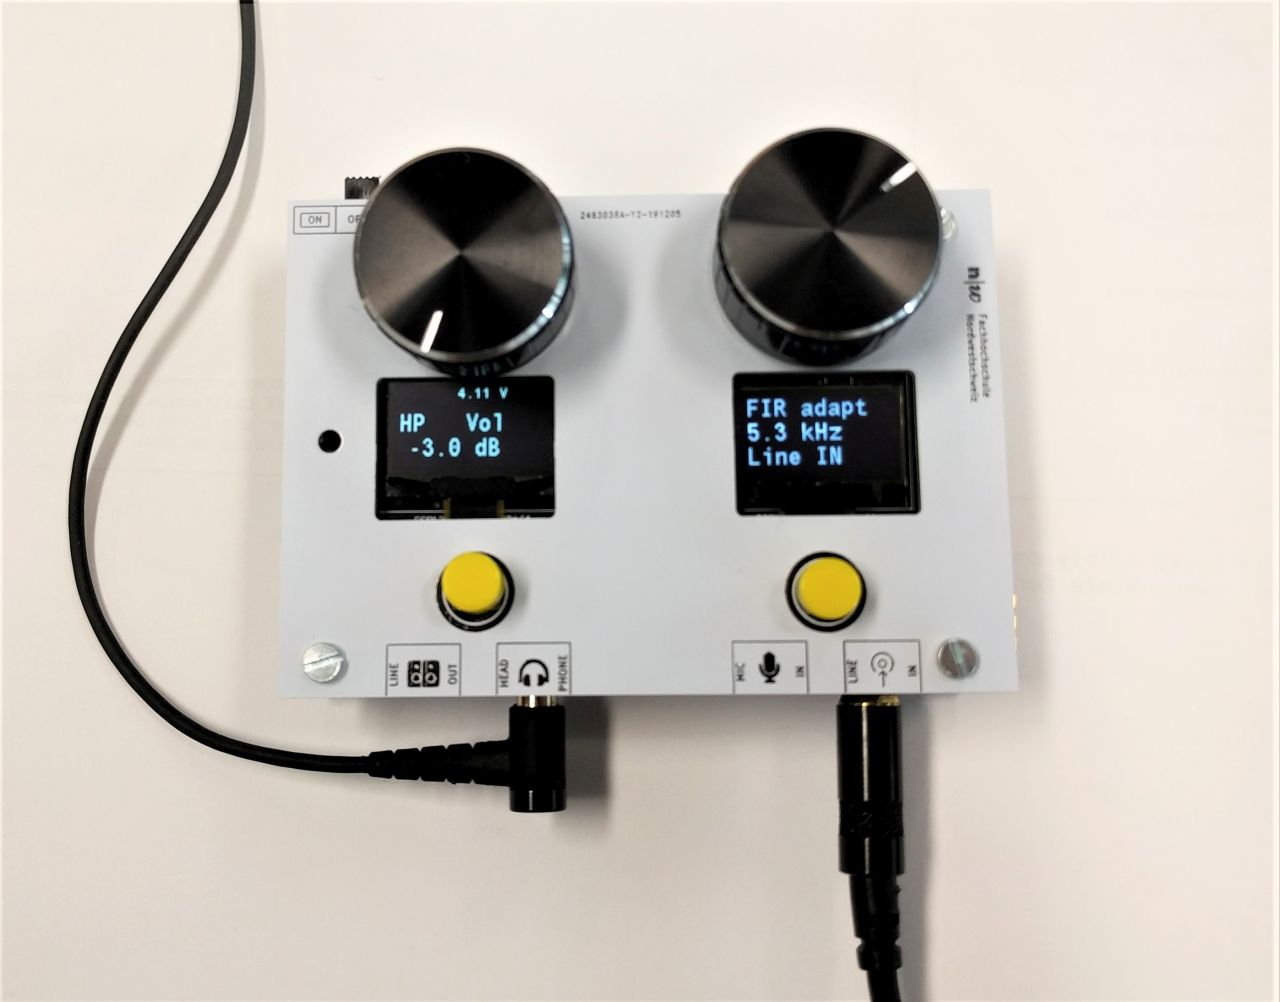
\includegraphics[scale=0.3]{dspboard_title}
		\end{figure}
		\begin{normalsize}
			{\begin{tabbing}
					\textbf{Betreuung:} \hspace{5cm}\= Prof. Dr. Markus Hufschmid\\
					
					%\\[0.8cm]
					%\textbf{Auftraggeber:} 
					%\>Prof. Dr. Markus Hufschmid\\
					
					\\[0.2cm]
					\textbf{Team:} \> Simon Burkhardt\\ 
					\> Mischa Studer\\
					%\\[0.8cm]
					\\[0.2cm]
					\textbf{Studiengang:} \>Elektro- und Informationstechnik
					\\[0.8cm]	\textbf{Semester:} \>Herbstsemester 2019
			\end{tabbing}}
		\end{normalsize}
		\vfill
	\end{center}
\clearpage

%%---ABSTRACT----------------------------------------------------------------------------
\selectlanguage{ngerman}				%ngerman or english
\thispagestyle{empty}
\begin{otherlanguage}{english}
\include{sections/abstract}
\end{otherlanguage}

%%---TABLE OF CONTENTS-------------------------------------------------------------------
\pagenumbering{Roman}		
\selectlanguage{ngerman}				%ngerman or english
\tableofcontents
\clearpage

%%---TEXT--------------------------------------------------------------------------------

\pagenumbering{arabic}
\section{Einleitung}
\label{sec:Einleitung}

Ein Amateurfunker hat während des Funkbetriebs immer wieder mit verschiedenen Störgeräuschen zu kämpfen die die Verständlichkeit der Verbindung erheblich beeinflussen. Genauso ist es für einen Hobbymusiker mühsam 19-Zoll Racks mit analogen Effekt-Geräten von Gig zu Gig zu schleppen, wenn er seine Musik nur mit ein paar simplen Audioeffekten versetzen möchte. In beiden Bereichen fehlt auch meistens das Budget und der Platz für teures analoges Equipment.\\
Hier bietet sich ein perfektes Anwendungsgebiet für digitale Signalverarbeitung. Jedoch sind auch handelsübliche digitale Effektgeräte meist nur für sehr spezifische Anwendungen konzipiert und kommen selten wirklich handlich daher.

Deswegen ist es das Ziel in diesem Projekt eine handliche DSP Einheit zu entwerfen, die mit einem schnellen modernen Microcontroller geeignete Effekte rechnen kann. Im Gegensatz zum Vorgängerprojekt, das mit einem dsPIC33 ausgestattet war und bis anhin im MicroCom Labor eingesetzt wurde, wird das neue Board mit einem ARM Cortex M4 Prozessor bestückt welcher dank seiner Floating-Point-Unit eine schnellere Verarbeitung von Signalen ermöglicht. Für die AD/DA-Wandlung sorgt ein TLV320 Codec um die Audio-Signale zuverlässig hin und her zu wandeln.

Die Vorteile einer Lösung  mittels Microcontroller sind so zahlreich wie offensichtlich. Dank der Vielseitigkeit der digitalen Signalverarbeitung können je nach Bedarf beliebige Effekte programmiert und auf das Board geflasht werden \footnote{In diesem Projekt ist es das Ziel die Hardware zu entwerfen und die Software soweit vorzubereiten, dass ein einfaches Audio-In/Audio-Out möglich ist. In einem späteren Projekt erst soll ein Tool entwickelt werden, welches die entsprechenden Effekte berechnet und aufs Board lädt.}. Der Prozessor inkl. Codec plus der Audio- und Kommunikations-Schnittstellen brauchen weder viel Platz, noch sind sie teuer. Die derzeitige Lösung ist auf einem 7x10cm PCB mit einem Budget-Rahmen von 50SFr realisiert worden. Ein DSP-Board mittels Microcontroller ist also die perfekte Lösung für Hobby-Anwendungen im Bereich Funk oder Musik.

Da die Bedienelemente mit je zwei Tasten, zwei Rotary Encoders und zwei 1.96inch Displays eher minimalistisch gehalten sind, können mehere DSP-Boards beliebig kaskadiert werden. Wie bei einem Puzzleteil werden die Boards ineinandergesteckt und über einen analogen Audio-Stecker wird das Signal von Board zu Board weitergeschlauft und weiterverarbeitet. So bleibt das System modular und kann für beliebige Anwendungen eingesetzt werden.

Das erarbeitete DSP-Board funktioniert erwartungsgemäss. Es ist möglich ein Audio-Signal einzuspeisen welches nach erfolgreicher AD/DA-Wandlung wieder am Audio-Ausgang anliegt. Die verschiedenen Ein-/Ausgänge sowie deren Pegel sind anwählbar über ein einfaches Menu. Zusätzlich wurde sogar ein FIR-Filter mit verstellbarer Grenzfrequenz implementiert.

%Kleine Fehler in der Analog-Schaltung haben sich eingeschlichen welche Verbesserungspotential bieten, jedoch keinen entscheidenden Einfluss auf die Funktion haben.

Die folgende Facharbeit ist in Analyse/Konzept, Hardware, Software, Validierung und Status/Verbesserungen unterteilt. Erst wird das angedachte Konzept grob erklärt und dessen Funktionsweise erläutert wonach detailliert auf die Umsetzung in den Teil-Bereichen Hardware und Software eingegangen wird. In den letzten beiden Kapiteln werden Teils-Systeme mit entsprechenden Messungen auf ihre Genauigkeit und Funktionalität untersucht und zum Schluss der momentane Status und mögliche Verbesserungen für weiterführende Projekte dargelegt.

%Das derzeit verwendete DSP Board für den Unterricht im MicroCom Labor basiert auf einem dsPIC33 mit Fixed-Point-Recheneinheit. Die neuen ARM Prozessoren bieten ab der Cortex-M4 Serie eine Floating-Point-Unit (FPU) und ermöglichen dadurch eine schnellere Verarbeitung von Signalen. \\
%
%Aus diesem Grund wird die Hardware des DSP Boards überarbeitet und soll mit einem ARM Cortex-M4 Microcontroller ausgestattet werden. Der Schaltungsaufwand beschränkt sich auf die wesentlichen Funktionen. Diese beinhalten die MCU, einen Codec für die AD/DA Wandlung, die Audio-Steckverbinder und die Bedienelemente des HMI. \\
%
%Im Bereich Amateurfunk und Hobbymusik besteht oft ein Bedürfnis nach einer einfachen Möglichkeit, ein Audiosignal mit einem Effekt zu verändern.
%So kann es sein, dass ein Amateurfunker mit einem Notch-Filter einen Störton unterdrücken möchte. Als Musiker möchte man mit einer Effektbox einen Reverbeffekt erzeugen.
%Effektgeräte und Filter am Markt sind oft zu einem Premiumpreis erhältlich.
%Dieses Projekt hat zum Ziel, eine günstige Alternative zu diesen Geräten zu bieten.
%
%
%Heute bieten die DSP Funktionen in der ARM Cortex-M4 Architektur einegünstige Möglichkeit Signalverarbeitung auf Microcontrollerebene zu betreiben. 
%Der Rahmen dieses Projektes umfasst die Entwicklung der Hard- und Firmware eines DSP Boards mit ARM Cortex-M4 Microcontroller. 
%Das Gerät wird mit Bedienelementen wie 2 Dreh


\clearpage
\section{Analyse und Konzept}
\label{sec:Analyse_Kozept}

Die mit dem betreuenden Fachdozenten Prof. Dr. Markus Hufschmid erarbeiteten Projektziele sind im Pflichtenheft hinterlegt (einzusehen im Appendix \ref{app:Pflichtenheft}).  Nachfolgend ist das erarbeitete Lösungskonzept näher erklärt welches zur Erreichung selbiger führen sollte.

	\subsection{Produktbeschreibung}
\label{sec:Produktbeschreibung}






%	
\section{Ziele}
\label{sec:Ziele}

\subsection{Harte Ziele}

\begin{table}[H]
\begin{tabular}{|l|l|l|ll}
\cline{1-3}

\textbf{Nr} & \textbf{Ziel} & \textbf{Erreichungsgrad} &  &  \\ \cline{1-3}
1.1         & Microcontroller mit Coretx-M4F Architecktur & erfüllt/nicht erfüllt    &  &  \\ \cline{1-3}
1.2         & Audio Passthrough von Line-In nach Line-Out                                                     & erfüllt/nicht erfüllt    &  &  \\ \cline{1-3}
1.3         & \begin{tabular}[c]{@{}l@{}}Audio Schnittstelle (analog) \\ - Line-IN \\ - Line OUT\end{tabular} & erfüllt/nicht erfüllt    &  &  \\ \cline{1-3}
1.4         & 2 Stk. Drehencoder für HMI                                                                      & erfüllt/nicht erfüllt    &  &  \\ \cline{1-3}
1.5         & 2 Stk. Taster für HMI                                                                           & erfüllt/nicht erfüllt    &  &  \\ \cline{1-3}
1.6         & 1 Display zur Anzeige des Funktionsmodus                                                        & erfüllt/nicht erfüllt    &  &  \\ \cline{1-3}
1.7         & Microcontroller ohne Debugger über USB programmierbar                                           & erfüllt/nicht erfüllt    &  &  \\ \cline{1-3}
\end{tabular}
\end{table}

\subsection{Weiche Ziele}

\begin{table}[H]
\begin{tabular}{|l|l|l|ll}
\cline{1-3}
\textbf{Nr} & \textbf{Ziel}                                                                                   & \textbf{Erreichungsgrad} &  &  \\ \cline{1-3}
2.1         & Anzahl Layer der Leiterplatte                                                     & ${n_{Layer} \leq 2}$    &  &  \\ \cline{1-3}
2.2         & \begin{tabular}[c]{@{}l@{}}Bauteile sind Handbestückbar \\ - SMD passiv $\geq$ 0603 \\ - SMD cases: keine QFN / BGA\end{tabular} & erfüllt/nicht erfüllt &  &  \\ \cline{1-3}
2.3         & Stromverbrauch erlaubt Betrieb über USB 2.0 Speisung & ${I_{USB} \leq 0.5A}$    &  &  \\ \cline{1-3}
2.4         & \begin{tabular}[c]{@{}l@{}}Audio Schnittstelle (analog) \\ - Headphone OUT \\ - Microphone IN\end{tabular} & erfüllt/nicht erfüllt    &  &  \\ \cline{1-3}
2.5         & \begin{tabular}[c]{@{}l@{}} Audio Verbindung (digital) \\ - IN / OUT Board-to-Board Kommunikation \\ Kaskadierung mehrerer Boards\end{tabular} & erfüllt/nicht erfüllt    &  &  \\ \cline{1-3}
2.6         & Akkubetrieb möglich & erfüllt/nicht erfüllt    &  &  \\ \cline{1-3}
2.7         & zusätzliche (farbige) LEDs als Anzeige des Betriebsmodus & erfüllt/nicht erfüllt    &  &  \\ \cline{1-3}
2.8         & Materialkosten inkl. PCB pro Stück bei 10 Stk. & ${k \leq 50 CHF}$    &  & \\ \cline{1-3}
\end{tabular}
\end{table}

\subsection{Nicht Ziele}

\begin{table}[H]
\begin{tabular}{|l|l|l|ll}
\cline{1-3}
\textbf{Nr} & \textbf{Ziel}                     & \textbf{Erreichungsgrad} &  &  \\ \cline{1-3}
3.1         & DSP Board für den Unterricht      & erfüllt/nicht erfüllt    &  &  \\ \cline{1-3}
3.2         & Aufwändiges Gehäuse               & erfüllt/nicht erfüllt    &  &  \\ \cline{1-3}
\end{tabular}
\end{table}

   % gehören nicht in den Fachbericht 
	\subsection{Lösungskonzept}
\label{sec:Loesungskonzept}

In diesem Abschnitt werden die Anforderungen and die einzelnen Teilaspekte aufgelistet und die Spezifikationen mehrerer Varianten verglichen.



		\subsubsection{Anforderungen an Microcontroller}
\label{sec:Konzept_Microcontroller}

Die an den Prozessor gestellten Anforderungen sind ein ARM-Cortex M4 Core mit DSP und FPU sowie Schnittstelle(n) zur Kommunikation mit dem Audio Codec. 
Dabei wird aufgrund der genaueren Samplingrate der Codec als Master betrieben und der DSP als Slave.
Der DSP muss also keine genaue Clock zur Verfügung stellen. 
Auf eine Cortex-M7 Architektur wird verzichtet, weil ab diesem Punkt auch ein Single-Board Computer (vgl. Raspberry Pi) eingesetzt werden kann.
Eine Tacktfrequenz von 200MHz ist wünschenswert, jedoch befinden sich die Cortex-M4 Prozessoren mit 200MHz auf dem selben Preisniveau von Cortex-M7 Microcontrollern.



		\subsubsection{Konzept USB Akkuladeregler IC}
\label{sec:Konzept_Charger}

Ein weiches Ziel ist die Autonomie ohne externe Energieversorgung. 
Dazu soll ein Akkumulator genügend Energie liefern, um die Schaltung während einiger weniger Stunden (live-Konzert) zu betreiben. 
Der Ladestrom soll nicht grösser als die über USB-2.0 zugelassenen $2.0\si{A}$ betragen.





		\subsection{Kaskadierung mehrerer Boards}
\label{subsec:Konzept_Kaskadierung}

Mehrere DSP-Boards sollen untereinander kaskadierbar sein, um das bearbeite Audio-Signal auf einem nächsten Board weiter zu verarbeiten. Auf eine digitale Schnittstelle wird in Absprache mit dem Auftraggeber, wegen der aufwändigen Clock-Synchronisation verzichtet. Das Signal wird analog weitergereicht, was in mehr analogem Rauschen resultiert. Dieser Effekt wird durch die kurzen Leitungen von Board zu Board minimal gehalten. Da die Gefahr besteht, dass der Benutzer jeweilige Link-Kabel verlegt oder zumindest nicht in nützlicher Frist zur Hand hat, wird die Kaskadierung mit einer Steckverbindung gelöst. Dabei werden zwei Boards direkt nebeneinander (Kante an Kante) zusammengesteckt.


\begin{table}[H]
	\centering
	\begin{tabular}{|c|c|c|c|}
		\hline
		\textbf{Specification} & \textbf{Mill-Max 868}             & \textbf{Pin Header 2x3} & \textbf{AVX 9159} \\ \hline
		Preis         & 5.26 + 7.00 (F/M 3P.)& 1.50 + 0.80 (M/F 6P.)&1.05 + 0.78 (F/M 3P)         \\ \hline
	\end{tabular}
	\caption{Preisvergleich der analogen Steckverbinder}
	\label{tab:stecker}
\end{table}

Da die verschiedenen Steckverbinder in \ref{tab:stecker} in Anzahl Leitungen alle das gleiche bieten, ist hier vor allem der Preis entscheidend. Der \textbf{AVX 9159}, welcher ursprünglich für LED-Schienen eingesetzt wird, ist mit Abstand der günstigste und eignet sich ebenso für eine Audio-Anwendung.



%Das Audio Signal wird von einem Board zum nächsten jeweils analog weitergereicht. 
%Der Steckverbinder soll kleiner als D-Sub sein. 
%Auf eine digitale Schnittstelle wird in Absprache mit dem Auftraggeber,  wegen der aufwändigen Clock-synchronisation und der Kosten für Steckverbinder (vgl. Optisch Toslink) verzichtet. 
%
%\todo{SB: Kaskadierungskonzept
%Weitergabe von analogem Signal und dadurch entstehendes mehrmaliges Wandeln ist unsauber aber analog ist einfach..oder so AVX-Stecker/Audio-Switch}

% technische Grundlagen ?

\clearpage
\section{Hardware}
\label{sec:Hardware}


	\subsection{Blockschaltbild}
\label{sec:Blockschaltbild}

\begin{figure}[H]
	\centering
	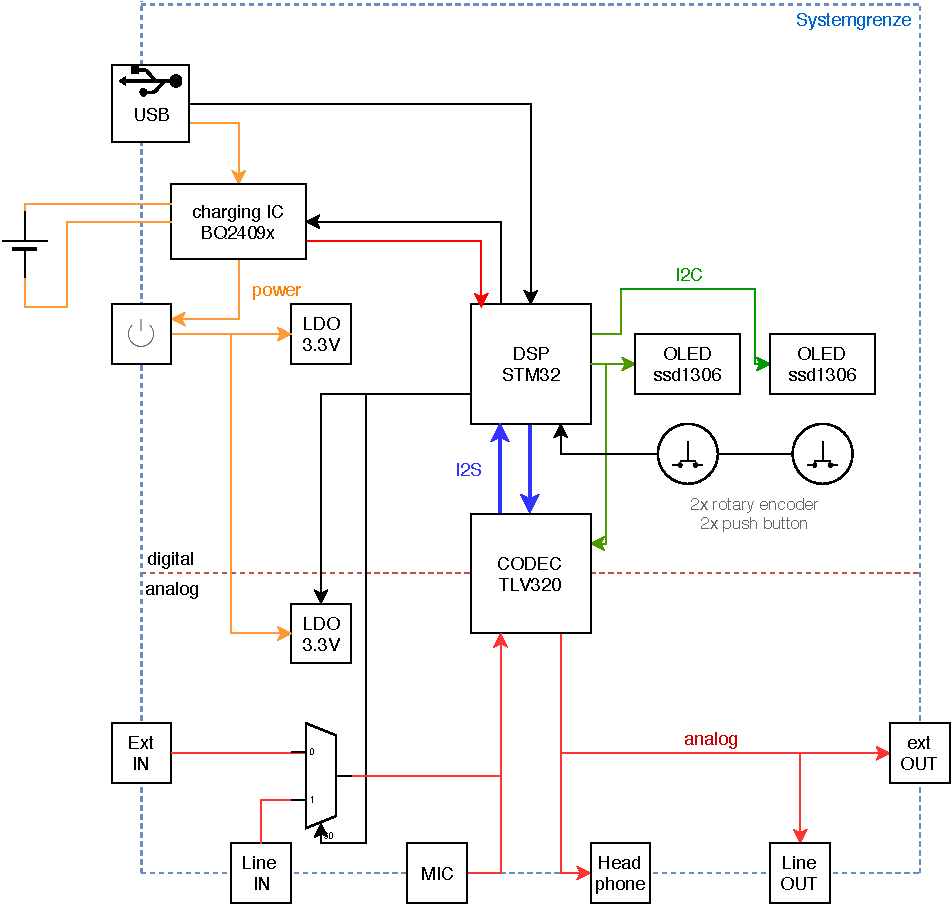
\includegraphics[width=0.8\linewidth]{block_diagramm}
	\caption{Blockschaltbild des DSP Boards}
	\label{pic:Blockdiagramm}
\end{figure}

Die Abbildung \ref{pic:Blockdiagramm} oben zeigt das Blockschaltbild mit den Komponenten um den DSP. Die Schaltung beinhaltet einen STM32 Microcontroller, dessen Beschaltung im Kapitel \ref{sec:Schema_DSP} dokumentiert ist. 
Als weitere Kernkomponente zählt der TLV320 Audio Codec, dessen Schema im Kapitel \ref{sec:Schema_Codec} beschrieben ist.

Zum Speisungsteil (orange) gehört ein Akkulade-IC (bq2409x), dessen Schaltung im Abschnitt \ref{sec:Schema_Speisung} beschrieben ist. Der Li-Ion/Li-Po Akkumulator ist auf dem Blockschaltbild ausserhalb des Systems gezeichnet und wurde im Rahmen dieses Projektes nicht evaluiert. Der bq2409x wurde gemäss Abschnitt \ref{sec:Valid_Batterie} mit einem Akkumulator getestet.





	\clearpage
	\subsection{Pegeldiagram}
\label{sec:Pegeldiagram}


	\clearpage
	\subsection{Schema}
\label{sec:Schema}

Das nachfolgende Kapitel zeigt das Schema des DSP Boards. 
In mehreren Unterkapiteln wird jeder Schaltungsteil im Detail beschrieben.
Berechnungen und Überlegungen sind bei den jeweiligen Teilaspekten aufgeführt.



		\subsubsection{Schema Speisung}
\label{sec:Schema_Speisung}

Nachfolgend wird der Speisungspfad vom USB mini-B Connector bis zu den Regulierten 3.3\si{V} beschrieben.

\paragraph{USB Port}

Ein standard USB 2.0 Port kann einen maximalen Strom von ${I_{max}=500\si{mA}}$ bereitstellen.
Dieser Strom ist die obere Grenze für das DSP Board. In keinem Betriebsfall inkl. Akkuladen wird dieser maximale Strom überschritten.
\
Zum Schutz der USB-Host Geräte vor einem Kurschlussstrom, ist F1 (MF-MSMF110) mit einem Auslösestrom von ${I_{trip}=2.20\si{A}}$ \cite{usb-fuse}.


\paragraph{Battery Management (BQ2409x)}

Der BQ24093 ist ein single-cell Li-Ion / Li-Po Akkulade-IC, das speziell für USB Applikationen gemacht ist.
Die Beschaltung des IC1 ist gemäss Vorgaben aus dem Datenblatt \cite{bq2409x}.

Der Akkumulator ist nicht Teil des Systems. Aus diesem Grund ist ein 2-Pin JST-XH Connector (J6) Vorgesehen.
Weil der Akkumulator und ein entsprechender temperaturabhängiger Widerstand nicht bekannt ist, 
wird der Pin für die Temperaturüberwachung mit R19 terminiert.
IC1 wird mit dem Pull-Down R51 am \texttt{ISET2} Pin auf \texttt{LOW} gezogen, was den Ladestrom auf ${I_{charge}=100\si{mA}}$ beschränkt. 
Bei Bedarf kann der Ladestrom vom STM32 über \texttt{PB14} auf \texttt{HIGH} und damit ${I_{charge}=500\si{mA}}$ festgelegt werden.


\begin{figure} [H]
\begin{center}
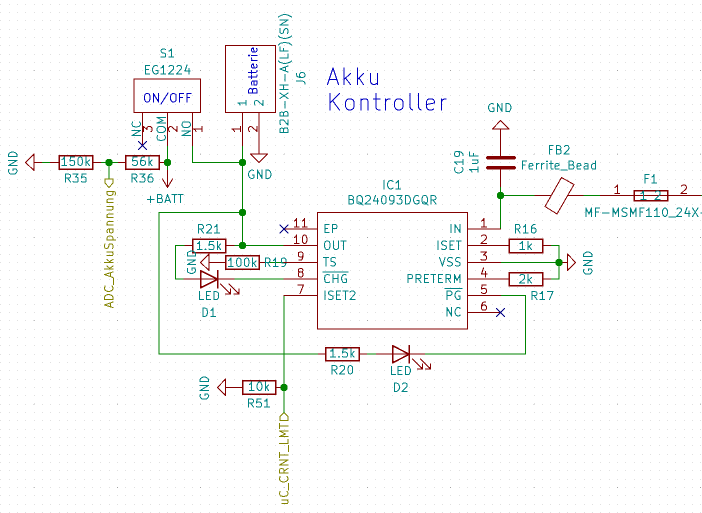
\includegraphics[scale=0.5]{../graphics/Schema_Akku.png}
\caption{BQ24093 mit äusserer Beschaltung nach Datenblatt}
\label{fig:Schema_Akku}
\end{center}
\end{figure}

\paragraph{ADC Akkumulator Spannungsmessung}

Die Akkumulatorspannung mit ${V_{bat}=4.2\si{V}}$ übersteigt den Eingangsspannungsbereich des\\
 STM32 Microcontrollers von ${V_{GPIO_{max}}=3.3\si{V}}$.
Damit zur Bestimmung des Ladestandes die Spannung gemessen werden kann, wird diese mit dem Spannungsteiler R35/R36 auf ein Maximum von 3.3\si{V} heruntergeteilt. 
Mit Widerstandswerten aus der E12-Reihe ergibt sich folgender Spannungsteiler.

\begin{equation}
V_{out_{max}} = V_{bat_{max}}*\frac{R35}{R35+R36}
\end{equation}

\begin{equation}
3.277\si{V} = 4.5\si{V}*\frac{150\si{k\Omega}}{150\si{k\Omega}+56\si{k\Omega}}
\end{equation}

Somit muss die gemessene Spannung in der Software um folgenden Faktor korrigiert werden.

\begin{equation}
F_C=\frac{V_{bat_{max}}}{V_{out_{max}}}=\frac{3.27\si{V}}{4.5\si{V}}=\underline{0.7\bar{3}}
\end{equation}

\paragraph{Energiebedarf der Schaltung}

Unten aufgeführt ist eine Abschätzung des Energiebedarfs der Schaltung, die massgebend für die Wahl der Spannungsregler ist. Die Speisung ist in analog und digital aufgeteilt.

\begin{table}[H]
\title{Stromverbrauch 3.3V digital}
\centering
\begin{tabular}{|l|r|}
\hline
\textbf{Schaltungsteil} & \textbf{Imax {[}\si{mA}{]}} \\ \hline
STM32                   & 40                     \\ \hline
SSD1306                 & 30                     \\ \hline
SSD1306                 & 30                     \\ \hline
reserve                 & 50                     \\ \hline
textbf{Total}           & \textbf{150}            \\ \hline
\end{tabular}
\end{table}

\begin{table}[H]
\title{Stromverbrauch 3.3V analog}
\centering
\begin{tabular}{|l|r|}
\hline
\textbf{Schaltungsteil} & \textbf{Imax {[}\si{mA}{]}} \\ \hline
MAX4762                 & 0.01                   \\ \hline
TLV320                  & 26.00                  \\ \hline
reserve                 & 30.00                  \\ \hline
textbf{Total}           & \textbf{56.01}          \\ \hline
\end{tabular}
\end{table}

Die verbauten Festspannungsregler TLC7333 (IC2, IC3) mit Low Dropout Voltage können bis zu ${I_{out}=300\si{mA}}$ liefern.

\paragraph{Verlustleistung der Spannungsregler}

Die maximale Verlustleistung an einem der Spannungsregler (IC2, IC3) tritt auf, wenn die Eingangsspannung ${V_{in}=5\si{V}}$ beträgt und der maximale Strom von ${I_{max}=0.15\si{A}}$ fliesst.
Dabei entsteht eine Verlustleistung von:\
\
${P_{LDO_{max}}=(5.0\si{V}-3.3\si{V})*0.15\si{A}}=0.255\si{W}$


\todo{ - soll man hier noch mit Pmax vom LDO vergleichen?}

		\subsubsection{Schema DSP}
\label{sec:Schema_DSP}

In diesem Abschnitt wird die Beschaltung des STM32F412 beschrieben. Für die genaue Pinkonfiguration, Pinfunktionen und Konfiguration dient das \\
Kapitel \ref{sec:CubeMX} "Konfiguration mit STM32CubeMX".
\\
\paragraph{I2S Schnittstelle}\vspace{-0.3cm}\\
Die Hersteller des TLV320 und des STM32 verwenden nicht die gleichen Signalbezeichnungen für das Pinout der Bauteile.
Die Tabelle \ref{tab:I2SPins} stellt den Bezug der Signale an beiden Chips her und zeigt die Signalrichtung und Verbindung wie sie im Schema des DSP Boards zur Anwendung kommt.

\begin{table}[H]
	\centering
	\begin{tabular}{|l|l|c|l|l|}
	\hline
	\textbf{STM32} & \textbf{Signal} & \textbf{Richtung}         & \textbf{Signal} & \textbf{TLV320} \\ \hline
	PC2            & MISO            & $\leftarrow$  & DOUT            & 6               \\ \hline
	PC3            & MOSI            & $\rightarrow$ & DIN             & 4               \\ \hline
	PB12           & WS              & $\rightarrow$ & LRCIN           & 5               \\ \hline
	PB12           & WS              & $\leftarrow$  & LRCOUT          & 7               \\ \hline
	PA2            & CKIN            & $\leftarrow$  & CLKOUT          & 2               \\ \hline
	\end{tabular}
	\caption{Signale zwischen dem DSP und dem Codec}
	\label{tab:I2SPins}
\end{table}

\paragraph{Bootloader und Bootpins}\vspace{-0.3cm}\\
Die STM32 Familie hat einen integrierten Firmware upgrade Bootloader.
Um diesen zu aktivieren müssen die externen BOOT[1:0] Pins im richtigen Muster gesetzt werden.
In diesem Projekt wird die Firmware über den USB mini-B Connector auf den STM32 überspielt.
Das Application Note AN2606 \cite[p.136]{AN2606} beschreibt die Pinkonfiguration für diesen Anwendungsfall.
So muss kein Pull-Up Widerstand an der \texttt{USB\_DP} Leitung angeschlossen sein um die OTG-Bedingungen zu erfüllen.
Ausserdem muss eine externe Clock mit einer Frequenz zwischen $4\si{MHz}$ und $26\si{MHz}$ verfügbar sein, was durch den externen Quartz \textit{Y1} erreicht wird.

Die Bootpins müssen gemäss der Application Note AN2606 \cite[Table 2]{AN2606} mit dem Boot Pattern 1 gesetzt werden um den DFU Bootloader zu starten.
Unten in der Tabelle sind die beiden Boot Modi zusammengefasst.

Der BOOT1 Pin ist beim STM32F412 auf PB2.

\begin{table}[H]
\centering
\begin{tabular}{|l|c|c|}
\hline
\textbf{Boot Mode} & \textbf{BOOT1} & \textbf{BOOT0} \\ \hline
Bootloader         & 0              & 1              \\ \hline
Normal             & 0              & 0              \\ \hline
\end{tabular}
\caption{Mode Auswahl über BOOT[1:0] Pins}
\end{table}

\paragraph{Bootstrap Schaltung für Bootpin}\vspace{-0.3cm}\\
Der STM32 ist fähig, per Software in den Bootloader Modus zu wechseln \cite{STM32-Softreset-Stackoverflow}. Die Software dazu ist jedoch aufwändiger als den Bootvorgang per Hardware auszulösen.

Aus diesem Grund ist der \texttt{BOOT0} Pin mit einem GPIO Pin (\texttt{PD2}) verbunden, Abbildung \ref{fig:Schema_Bootpin_Bootstrap}.

\begin{figure} [H]
	\begin{center}
		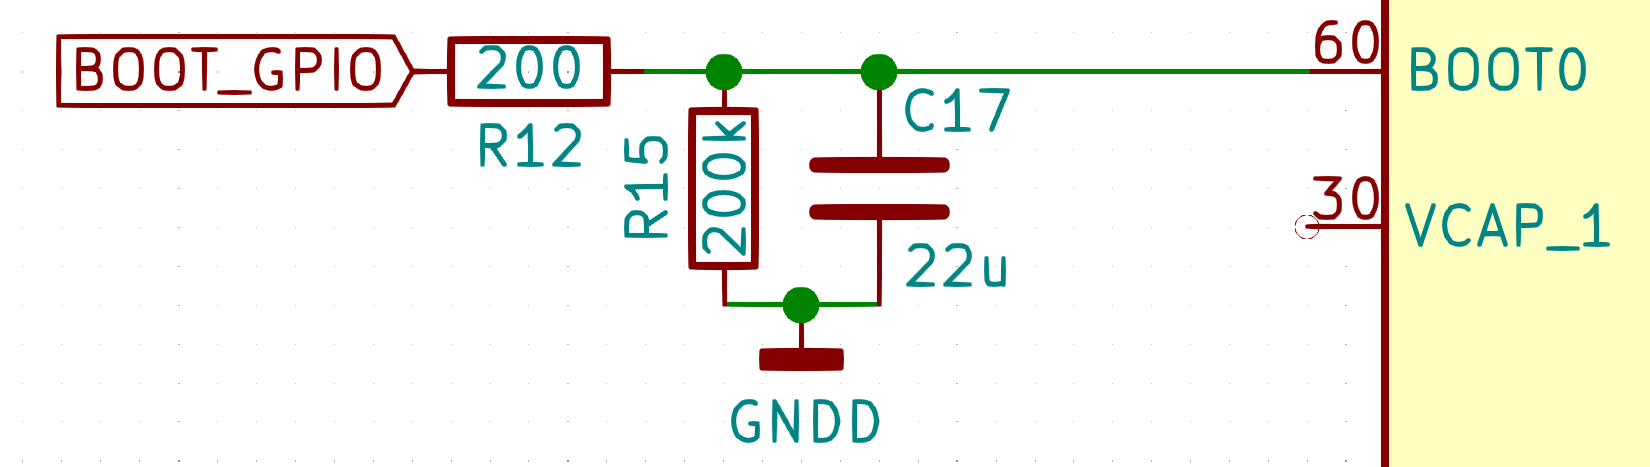
\includegraphics[scale=0.5]{../graphics/Schema_Bootpin_Bootstrap}
		\caption{Beschaltung des \texttt{BOOT0} Pins um über einen GPIO den Bootmodus zu setzen}
		\label{fig:Schema_Bootpin_Bootstrap}
	\end{center}
\end{figure}

So kann per Software der GPIO \texttt{PD2} auf \texttt{HIGH} gezogen werden und ein Software-Reset ausgelöst werden (siehe Abschnitt \ref{sec:Enter_DFU} in der Software), damit der STM32 im DFU-Bootloader startet.
Um dem Controller genügend Zeit zum Booten zu verschaffen, ist der \texttt{BOOT0} Pin mit einem $22\si{\mu F}$ Kondensator abgestützt. Der maximale Ausgangsstrom für einen GPIO beträgt $I_{GPIO}=25\si{mA}$ \cite[Table 14]{STM32f412}.
Mit dem Widerstand \textit{R12} beträgt der maximale Strom bei ungeladenem Kondensator \textit{C17}: 

\begin{equation}
I_{GPIO_{max}}=\frac{V_{CC}}{R_{12}}=\frac{3.3\si{V}}{200\si{\Omega}}=16.5\si{mA}
\end{equation}

Der Kondensator \textit{C17} wird über \textit{R15} entladen. Dabei bleibt dem STM32 ungefähr $1\tau=R*C$ Zeit um zu rebooten und den korrekten Pin-Zustand einzulesen. Diese Zeit beträgt ungefähr:

\begin{equation}
t_{reboot_{max}} \approx \tau = R_{15}\cdot C_{17} = 200\si{k\Omega}\cdot 22\si{\mu F}=220\si{ms}
\end{equation}
\\
\paragraph{Rotary Encoder und Buttons}\vspace{-0.3cm}\\
Einige Timer des STM32 unterstützen einen Encoder Modus, bei dem zwei GPIO Inputs zum Zählen der Encoderpulse verwendet werden können.

Alle 4 Pushbuttons sind an interruptfähige (EXTI) GPIO Pins angeschlossen. 
Die STM32 Familie unterstützt externe GPIO Interrupts an allen Pins. 
Dabei stehen 16 Interrupt Channels zur Verfügung, von welchen die Channel Nummer jeweils mit der GPIO Port Nummer übereinstimmen muss. 
Wie in der nachfolgenden Tabelle \ref{tab:EXTIPins} aufgeführt, werden insgesamt 6 EXTI Channels belegt.

\begin{table}[H]
	\centering
	\begin{tabular}{|l|l|r|}
	\hline
	\textbf{Signal}  & \textbf{GPIO} & \textbf{EXTI} \\ \hline
	Encoder 1 Button & PC12          & 12            \\ \hline
	Encoder 2 Button & PB13          & 13            \\ \hline
	Button 1         & PA0           & 0             \\ \hline
	Button 2         & PA1           & 1             \\ \hline
	Line In Detect   & PC14          & 14            \\ \hline
	MIC In Detect    & PC15          & 15            \\ \hline
	\end{tabular}
	\caption{GPIO Mapping auf EXTI Interrupt Channels}
	\label{tab:EXTIPins}
\end{table}





		\subsubsection{Schema Codec}
\label{sec:Schema_Codec}

Die Wandlung des analogen Audio-Signale sowie die Rückwandlung der digitalen Signale vom Microcontroller  übernimmt ein TLV320AIC23B von Texas Instruments. Dieser Codec hat eine variable Sampling-Frequenz (8kHz-96kHz), einen Köpfhörer- und einen Mikrofon-Vorverstärker. Die Register des Codecs werden über I2C programmiert (wobei auch SPI möglich wäre), dazu wird der Mode-Pin über einen Widerstand auf GND gezogen. Die gesampelten Daten wiederum werden über I2S an den Microcontroller übermittelt. Zusätzlich wird der 12.28 \si{MHz} Audio-Clock mit dem der Codec taktet von einem externen ECS-Quartz erzeugt (Abbildung \ref{fig:Schema_Codec}). 

\begin{figure} [H]
\begin{center}
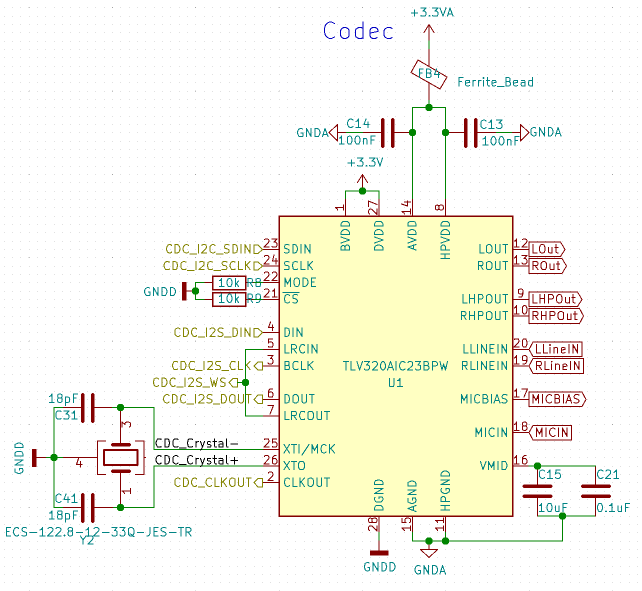
\includegraphics[scale=0.5]{../graphics/Schema_Codec.png}
\caption{TLV320AIC23B Codec von Texas Instruments}
\label{fig:Schema_Codec}
\end{center}
\end{figure}

Die Analog-Speisung des TLVs wird neben den 100\si{nF} Stütz-Kondensatoren zusätzlich von einem Ferrit Bead geglättet. Damit wird sichergestellt, dass keine ungewollten hochfrequente Spitzen in der Speisung das Audio-Signal verfälschen.

In den nachfolgenden Unterkapiteln wird genauer auf die In- und Outputs des DSP-Boards, beziehungsweise deren äusseren Beschaltung eingegangen.


\paragraph{Line Input}
\label{par:LineIN}
Das Line-Signal wird am Eingang (Abbildung \ref{fig:Schema_LineIN}) erstmal durch den Spannungsteiler mit \textit{R23} und \textit{R14} bzw. \textit{R27} und \textit{R26} halbiert. Im Datenblatt des TLV320AIC23B \cite{tlv320} wird empfohlen die Signal-Amplitude von 2V auf 1V runterzubringen. Zudem bilden \textit{R23/R26} zusammen mit \textit{C23/C26}  einen Tiefpass-Filter mit einer Grenzfrequenz von 604.7 MHz, was schonmal die gröbsten hochfrequenten Störungen filtert. Mit \textit{C24/C20} wird das Signal zusätzlich galvanisch entkoppelt.

\begin{figure} [H]
\begin{center}
 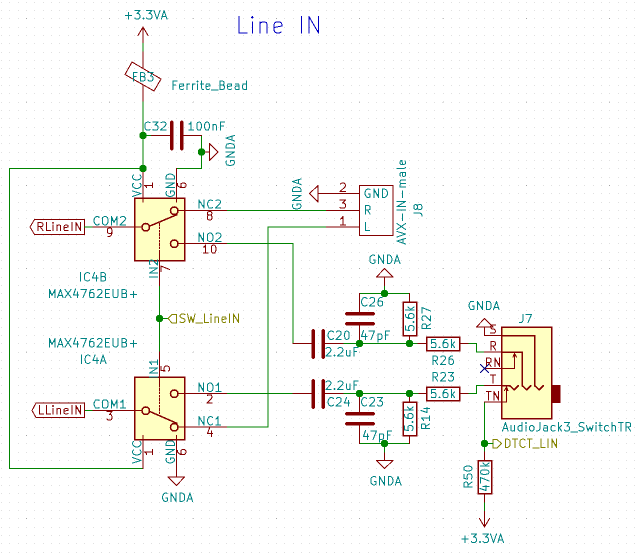
\includegraphics[scale=0.5]{../graphics/Schema_LineIN.png}
\caption{Line Eingangsstufe mit Audio-Switch}
\label{fig:Schema_LineIN}
\end{center}
\end{figure}

Parallel dazu kommt über einen AVX-Stecker alternativ ein Audio-Signal von einem nächsten DSP-Board rein. Die Auswahl des Line-In Signals erfolgt über einen MAX4762 \cite{max4762} Audioswitch von Maxim.

\paragraph{Line Output}
\label{par:LineOUT}

\begin{figure} [H]
\begin{center}
 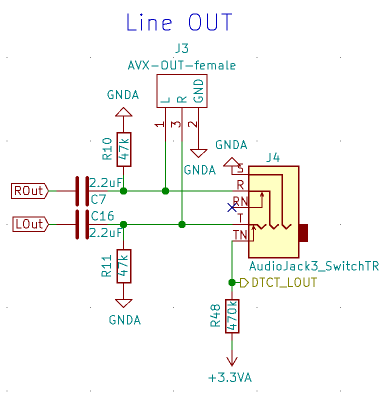
\includegraphics[scale=0.5]{../graphics/Schema_LineOUT.png}
\caption{}
\label{fig:Schema_LineOUT}
\end{center}
\end{figure}


\paragraph{Headphone Output}
\label{par:HPOUT}


\begin{figure} [H]
\begin{center}
 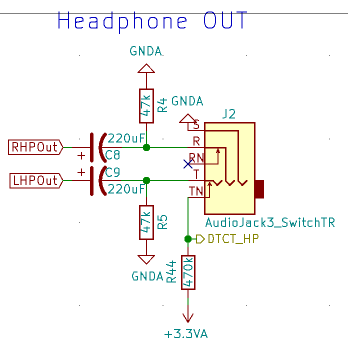
\includegraphics[scale=0.5]{../graphics/Schema_HPOUT.png}\caption{}
\label{fig:Schema_HPOUT}
\end{center}
\end{figure}




\paragraph{Mikrofon Input}
\label{par:MicIN}

\begin{figure} [H]
\begin{center}
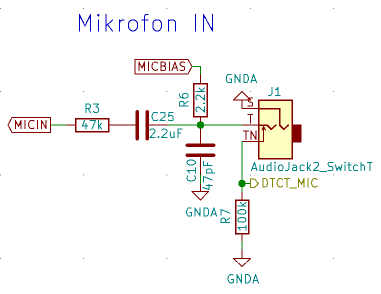
\includegraphics[scale=0.5]{../graphics/Schema_MicIN.png}
\caption{}
\label{fig:Schema_MicIN}
\end{center}
\end{figure}

\begin{figure} [H]
\begin{center}
 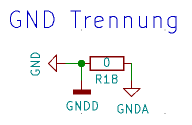
\includegraphics[scale=0.5]{../graphics/Schema_GND.png} 
\caption{}
\label{fig:Schema_GND}
\end{center}
\end{figure}



 
	\newpage
\subsection{PCB}
\label{sec:PCB}

Im nachfolgenden Kapitel wird näher erläutert wie das PCB aufgebaut ist und worauf geachtet wurde.

Grundsätzlich ist das Board in zwei fundamentale Teile eingeteilt (ersichtlich in Abbildung \ref{fig:PCB_GNDVDD}).  Den Digital-Teil inklusive Speisung, Microcontroller und den digitalen Schnittstellen. Und den Analog-Teil mit dem Codec und den verschiedenen Ein- und Ausgängen. In beiden Teilen wird rückseitig separat die Ground-Fläche geführt. Die beiden Flächen sind, wie in \ref{par:GND} erläutert, an genau einem Punkt durch einen $0\Omega$ Widerstand verbunden. Um die Speisungen grösstmöglich zu führen sind vorderseitig die beiden Teile mit 3.3VA beziehungsweise 3.3VD ausgegossen (nachdem alle Verbindungen gezogen worden sind).

\begin{figure} [H]
\begin{center}
 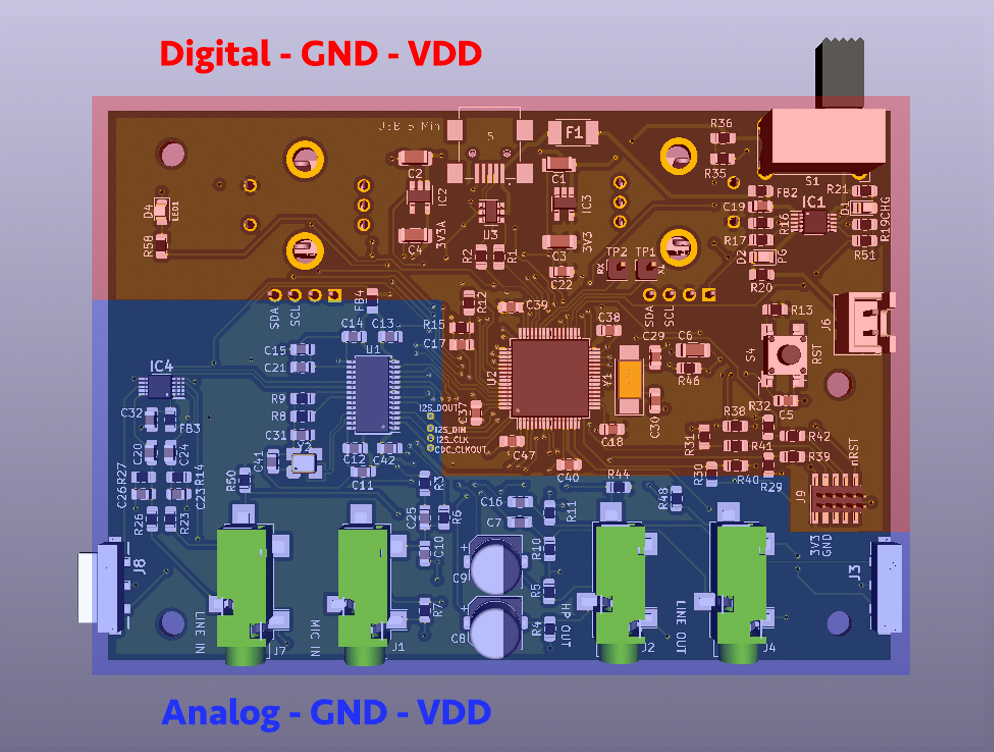
\includegraphics[scale=0.35]{../graphics/PCB-Layout_GNDVDD.jpg}
 \caption{Die Unterteilung des PCBs in Analog- und Digital-Teil}
\label{fig:PCB_GNDVDD}
\end{center}
\end{figure}

Im Speisungs-Teil ist wichtig, dass keine Speisungs-Schleifen entstehen. Die  Speiseleitungen sind zudem doppelt so breit wie die restlichen Leitungen (0.5mm), um den maximalen Strom von 500mA auszuhalten.

\begin{figure} [H]
\begin{center}
 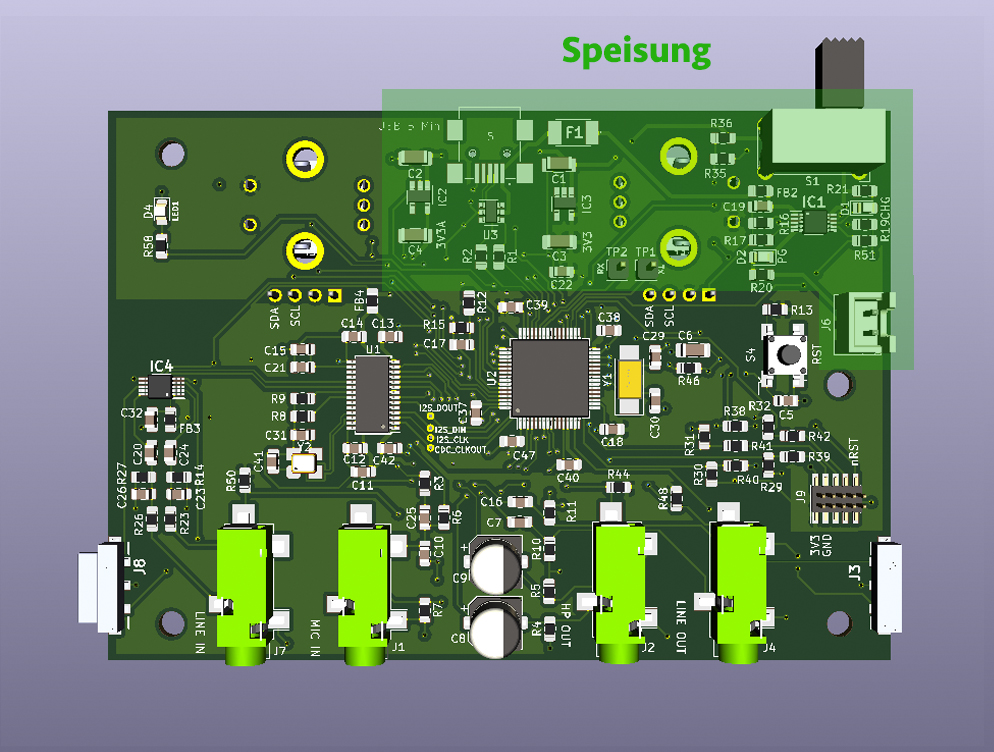
\includegraphics[scale=0.35]{../graphics/PCB-Layout_PWR.jpg}
 \caption{Die Speisung des PCBs mit der Mini-USB-Buchse, dem Lade-IC für den Akku sowie den beiden LDOs für Digital- sowie Analog-Teil}
\label{fig:PCB_PWR}
\end{center}
\end{figure}
Die räumliche Trennung verschiedener Teile auf dem PCB sollte mögliche gegenseitige Wechselwirkungen vermeiden oder zumindest vermindern. Speziell die Speisung und der Audio-Teil sind getrennt. Im Speisungs-Teil fliessen sicher die grössten Ströme auf dem ganzen Print, was mögliche EMV-Komplikationen nach sich ziehen kann. Im Audio-Teil würden im schlimmsten Fall solche Induktions-Spannungen als Signal interpretiert werden. Deswegen sind diese beiden Teile weitmöglichst voneinander entfernt, in den beiden Ecken, platziert.

\begin{figure} [H]
\begin{center}
 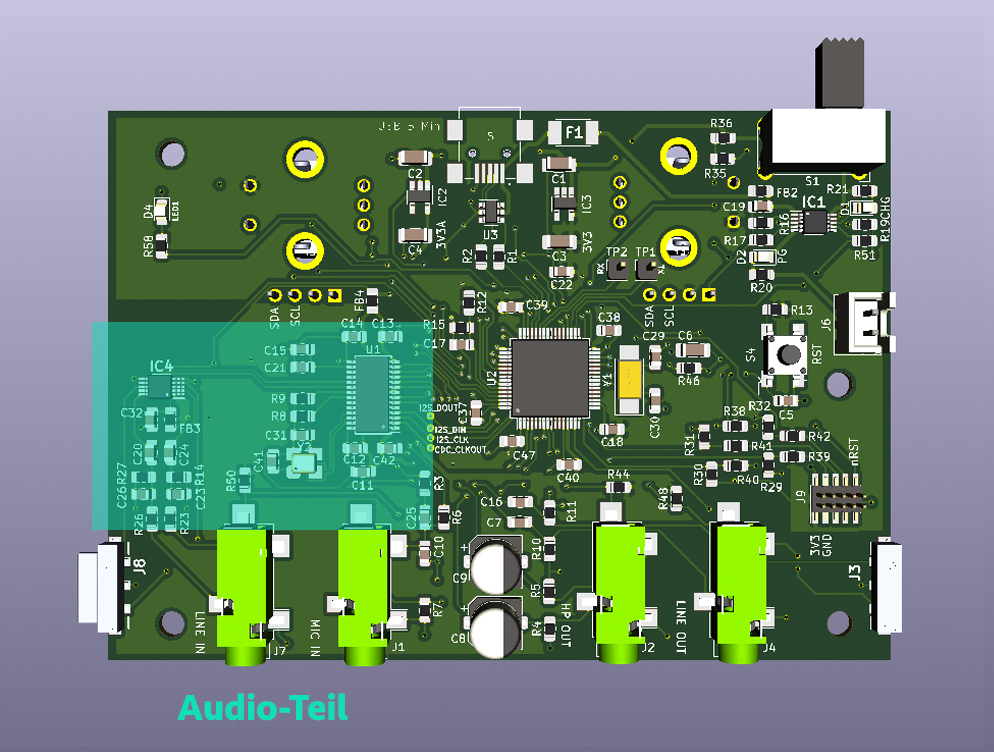
\includegraphics[scale=0.35]{../graphics/PCB-Layout_AUDIO.jpg}
 \caption{Der Audio-Teil mit dem Codec, dem Audio-Switch, dem 12.28MHz Quartz sowie der äusseren Beschaltung der Ein- und Ausgänge}
\label{fig:PCB_AUDIO}
\end{center}
\end{figure}

Im Audio-Teil sind zusätzliche Messpunkte zur Überprüfung der I\textsuperscript{2}S Kommunikation hinzugefügt, welche nur für den Prototyp vorgesehen sind. 

\begin{figure} [H]
\begin{center}
 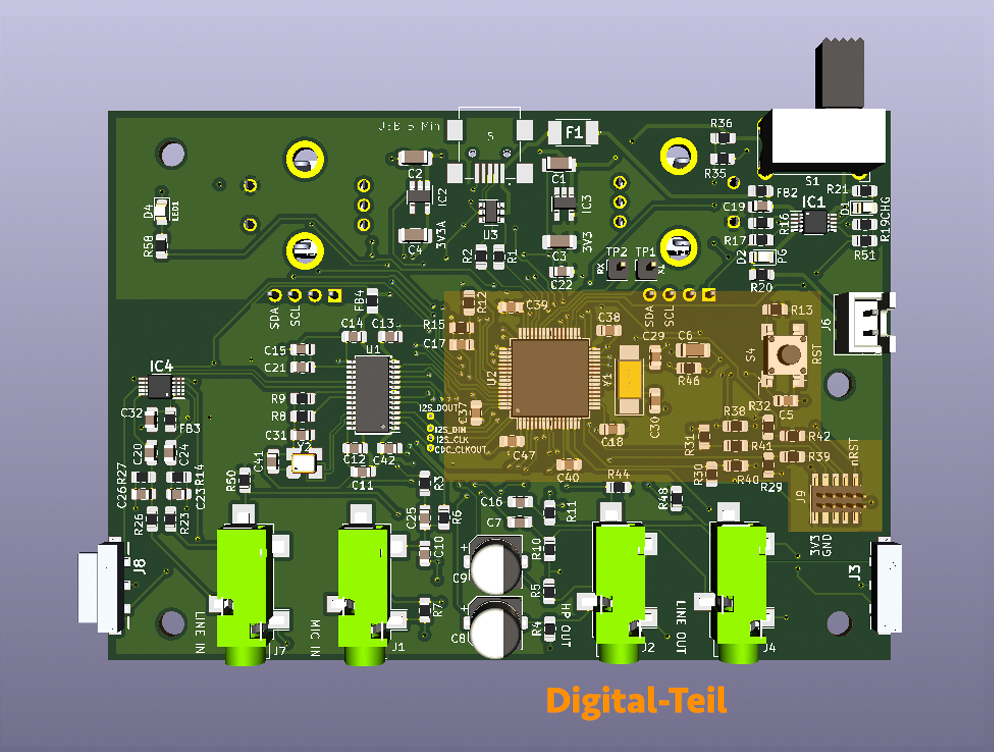
\includegraphics[scale=0.35]{../graphics/PCB-Layout_DGTL.jpg}
 \caption{Der Digital-Teil mit dem Mikrokontroller, dem 8MHz Quartz und der JTAG-Schnittstelle}
\label{fig:PCB_DGTL}
\end{center}
\end{figure}

Im Digital-Teil sind vor allem die Stützkondensatoren der Speisung und der 8MHz Quartz möglichst nahe an den Pins des Microcontrollers platziert. Für den Clock ist ein differenzielles Leitungspaar gezogent, ein Befehl in KiCad welcher bewirkt dass die beiden Leitungen exakt gleich lang werden. Dieser Befehl ist ebenfalls für den 12.28MHz des Audio-Teils und die Datenleitungen des USB-Steckers implementiert.

\begin{figure} [H]
\begin{center}
 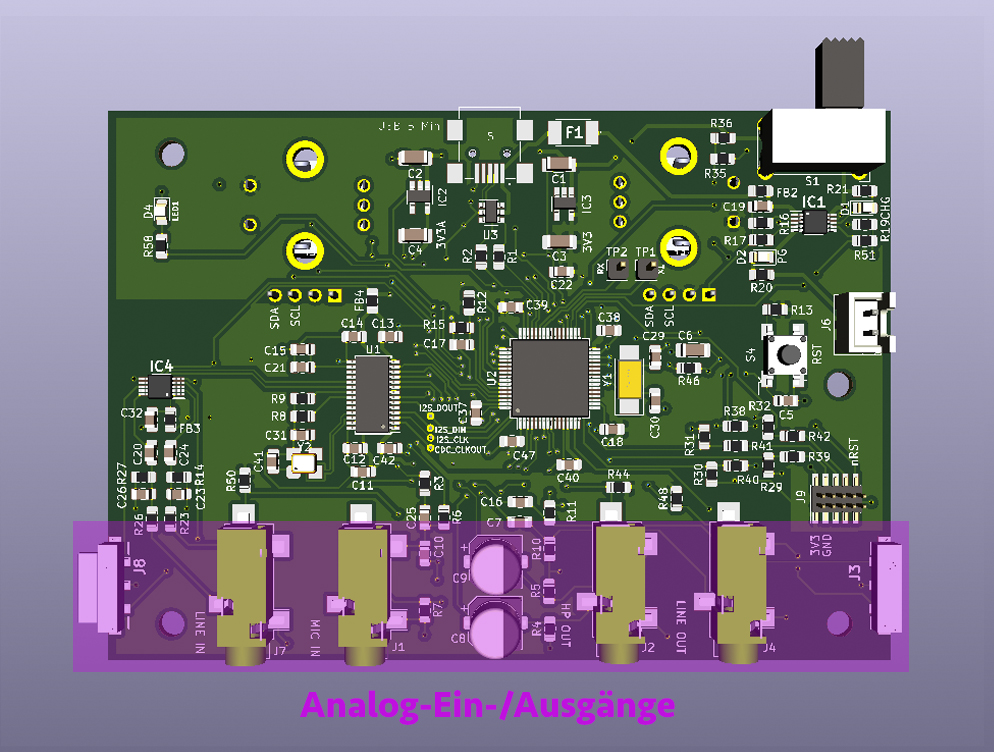
\includegraphics[scale=0.35]{../graphics/PCB-Layout_INOUT.jpg}
 \caption{Die Audio-Ein- und -Ausgänge mit 2x2 Mini-Jack Buchsen und 2 AVX-Verbinder für die Board-to-Board Verbindung}
\label{fig:PCB_INOUT}
\end{center}
\end{figure}

Mit dem Gedanken das Board später mit einem Gehäuse zu ergänzen sind die Ein-/Ausgänge, speziell die AVX-Stecker für die Board-zu-Board Verbindung, möglichst nahe am Rand platziert. Um es einheitlich zu halten, dient die untere Kante als Audio-Interface und die obere Kante als Digital-/Power-Interface. 

\begin{figure} [H]
\begin{center}
 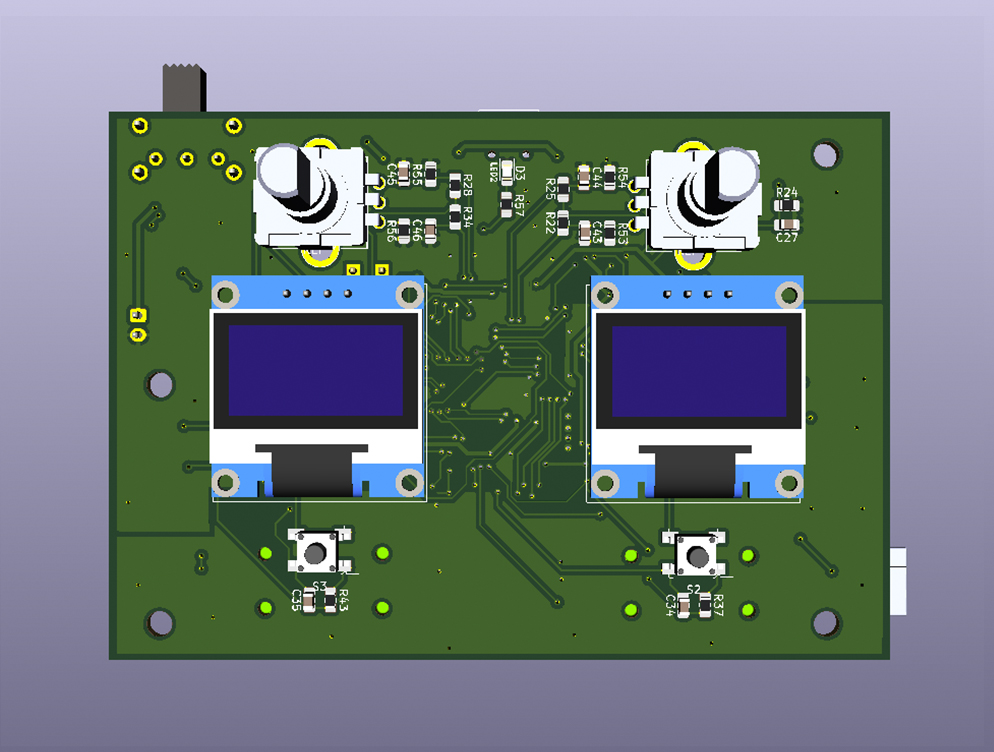
\includegraphics[scale=0.35]{../graphics/PCB-Layout_GUI.jpg}
 \caption{Die Bedienoberfläche mit je zwei Rotary-Encodern, Buttons und OLED-Displays}
\label{fig:PCB_GUI}
\end{center}
\end{figure}

Um Kosten zu sparen sind die Bedienelemente für das Benutzer-Interface gleich auf der Rückseite des PCBs angebracht.
	\subsection{Kosten}
\label{sec:Kosten}

Die Vorgabe des Auftraggebers bezüglich der Herstellungskosten für das DSP-Board beläuft sich auf eine Limite von 50SFr pro Board, bei einer Serie von 100 Stück. Die Kosten für die ersten fünf Prototypen haben diese Limite noch nicht eingehalten. Ein grosser Faktor ist hier jedoch der Stückpreis für die Herstellung des PCBs. Mit einer Serie vonn 100 Stück werden die PCB-Kosten jedoch massiv gesenkt.

\begin{table}[H]
	\centering
	\begin{tabular}{|r|r|r|r|}
		\hline
		\textbf{Serie} & \textbf{Bauteile /Board}             & \textbf{PCB /Board} & \textbf{Total /Board} \\ \hline
		5 Stück              &           47.7 SFr      & 21.8 SFr & 69.5 SFr    \\ \hline
		100 Stück           & 35.2 SFr                       & 4.7 SFr  & 39.9 SFr    \\ \hline
	\end{tabular}
	\caption{Die Kosten pro DSP-Board (bei verschiedenen Serien)}
	\label{tab:kosten}
\end{table}

Die Preise basieren auf dem Online-Shop Digi-Key \cite{www:digikey} für die Bauteile und Euro Crircuits \cite{www:eurocircuits} für das PCB.
Nicht eingerechnet  sind die Kosten für ein allfälliges Gehäuse, für einen zusätzlichen Akku und für die SMD-Widerstände. Letztere machen keinen signifikanten Unterschied (max 0.5 SFr) und sind in jedem ausgerüsteten Elektronik-Labor in grösseren Mengen verfügbar. Der Akku jedoch würde das Budget sprengen und ist entsprechend nur ein optionale Erweiterung.

\clearpage
\section{C Software}
\label{sec:Firmware}

Das Kapitel \ref{sec:Firmware} beschreibt die Entwicklungsumgebung, die Strukturierung des Softwareprojektes sowie die einzelnen Komponenten der Software.


	\subsection{User Interface des Demoprogramms}
\label{sec:GUI-Manual}

Auf dem DSP Board ist zu Demonstrationszwecken eine Demosoftware installiert.
Die Programmierung dieser Software ist in den folgenden Kapiteln beschrieben.
Der Abschnitt hier beschreibt die Funktionsweise des Demoprogramms für den Anwender.

Die Abbildung \ref{pic:P5-User-Interface} zeigt den Aufbau und die Zustände des einfachen Menus. Mittels Drücken der Encoder und Buttons können die Funktionen gewechselt werden.
Durch Drehen der Encoder können die Parameter der jeweils angezeigten Funktion verändert werden.

\begin{figure}[H]
	\centering
	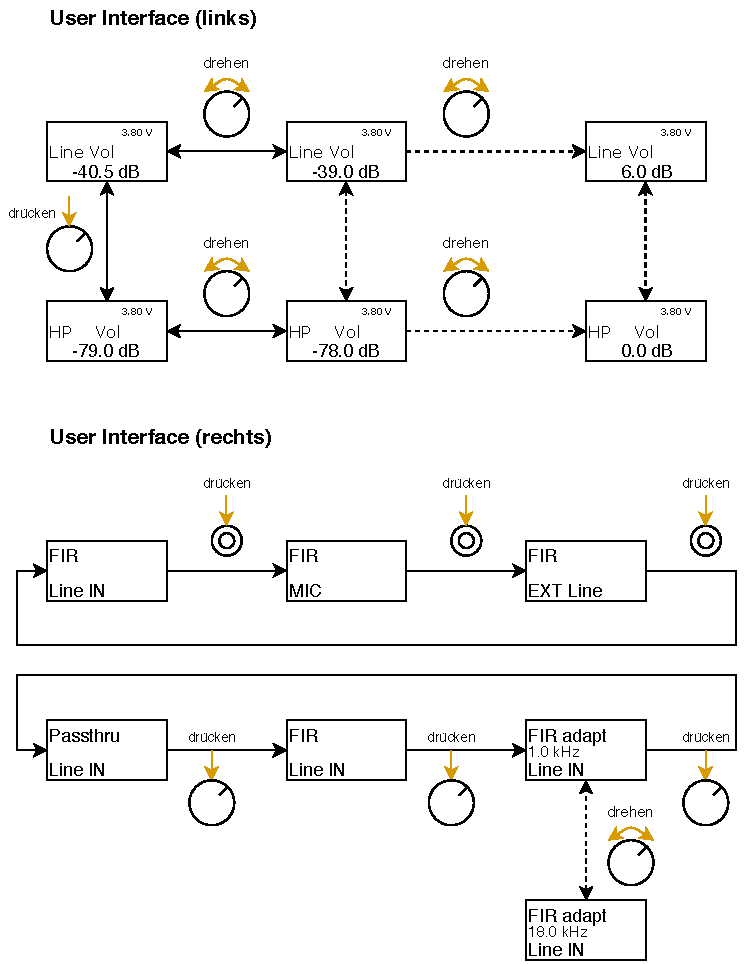
\includegraphics[width=0.75\linewidth]{P5-User-Interface}
	\caption{Das Diagramm zeigt die beiden OLED-Displays mit dem Menu und den Interaktionen}
	\label{pic:P5-User-Interface}
\end{figure}

Mit der linken Seite wird die Lautstärke für Line-Out und Headphone eingestellt.
Auf der rechten Seite, kann einerseits mit dem Button die Input-Quelle selektiert werden und andererseits mit dem Encoder die DSP-Funktion ausgewählt werden. 
Beim Menupunkt \glqq\textit{FIR adapt}\grqq \ kann zusätzlich die Grenzfrequenz des FIR Tiefpassfilters verändert werden.




	\subsection{Entwicklungsumgebung Keil uVision 5}
\label{sec:IDE}

Die Software ist in C mit der Keil uVision 5 IDE geschrieben. Nachfolgend ist beschrieben, welche Schritte unternommen werden müssen, um das Projekt erfolgreich zu kompilieren.

Die Handhabung eines Firmware-Upgrades über den USB-Anschluss am DSP-Board ist in Kapitel \ref{sec:USBDFU} beschrieben.
\\
\paragraph{Evaluation Modus bei Keil uVision 5}\vspace{-0.3cm}\\
Die IDE Keil uVision 5 kann im Eval Modus gratis verwendet werden.
Jedoch ist die kompilierte Code-Grösse auf $32\si{kB}$ beschränkt.
Die nachfolgende Tabelle \ref{tab:codesize} und das dazugehörige Listing zeigen den aktuellen Stand der Codegrösse.\\

\begin{lstlisting}[caption={Build Output beim Kompilieren der Software}]
linking...
Program Size: Code=22930 RO-data=6050 RW-data=196 ZI-data=9684  
FromELF: creating hex file...
"P5_Debug\P5_Debug.axf" - 0 Error(s), 0 Warning(s).
Build Time Elapsed:  00:01:00
\end{lstlisting}

\begin{table}[H]
	\centering
	\begin{tabular}{|l|l|}
		\hline
		Code Size Limit in Eval Mode & $32\si{kB}$ \\ \hline
		Compiled Code size DSP-Board & $23\si{kB}$ \\ \hline
	\end{tabular}
	\caption{Vergleich der Code Size mit dem vorgegebenen Limit}
	\label{tab:codesize}
\end{table}


		\subsubsection{Installieren und einrichten von Keil}
\label{sec:KeilInstall}

Dieser Abschnitt beschreibt die Installation von Keil uVision 5 mit den dazugehörigen Packages auf Windows.

	\subsection{Programmer und Debug Adapter (J-Link)}
\label{sec:SeggerJlink}

Um das DSP-Board zu flashen und debuggen kommt ein ARM Cortex fähiger Programmer zum Einsatz.
Dies kann beispielsweise ein ST-Link V2 von STMicroelectronics \cite{STLinkV2}, eine Black Magic Probe \cite{1bitBMP}.
In diesem Projekt kam ein \textit{J-Link EDU mini} von Segger\cite{JLinkEDU} zum Einsatz.
Der Einsatz dieses Programmers ist jedoch strikt auf den Gebrauch für Bildungszwecke eingeschränkt.

\subsubsection{J-Link Konfiguration in Keil uVision}

Damit der Flash-download und das Debugging richtig funktioniert, müssen in Keil uVision folgende Einstellungen vorgenommen werden.

\begin{figure}[H]
	\centering
	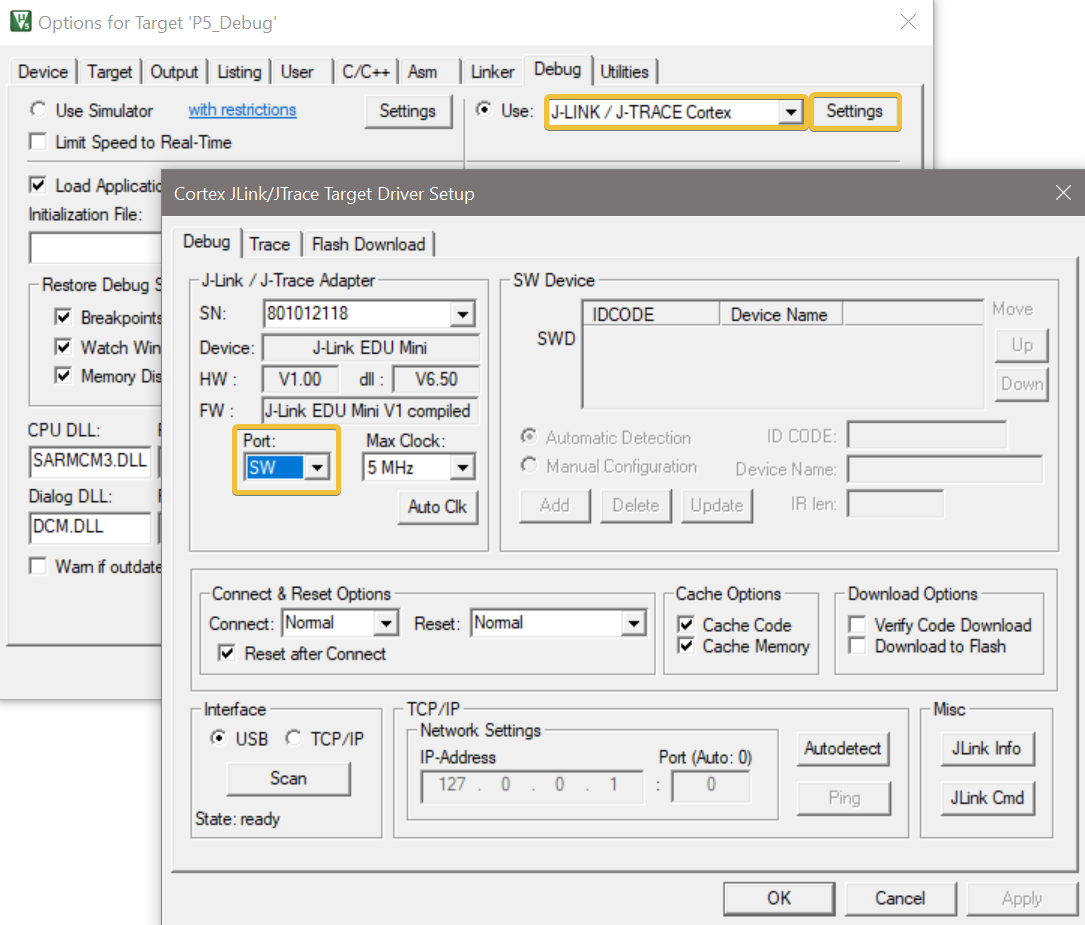
\includegraphics[width=0.9\linewidth]{keil-jlink}
	\caption{Project Properties mit den Einstellungen für den Segger J-Link im SWD Modus}
	\label{pic:keil-jlink}
\end{figure}

Die Abbildung \ref{pic:keil-jlink} zeigt das Fenster mit den Project Properties, das unter \texttt{Project > Options for Target 'DSP Board' > Debug} zu finden ist.
Hier muss "\textit{use J-Link/J-Trace}" ausgewählt und die Settings dazu geöffnet werden. 
Die Hardwareschnittstelle ist SWD und nicht JTAG.


	\subsection{Projektstruktur}
\label{sec:SWProjekt}

Die Dateistruktur des Softwareprojektes in Keil uVision 5 ist unten beschrieben. 
Es sind nur die Dateien erwähnt, die für die Entwicklung der Software massgebend sind.

\todo{Verlinkungen auf Unterkapitel}

\paragraph{main.c}

In der \texttt{main.c} Datei befindet sich der Hauptteil des Softwareprojektes.
Libraries werden inkludiert, glbale sowie lokale Variablen deklariert und die Initialisierung des STM32 und aller Peripherie aufgerufen.
Innerhalb der \texttt{while(1)} Schlaufe ist eine State Machine realisierbar, die den Programmablauf des User Interfaces bestimmt.
Viele Variablen sind global und \texttt{volatile} deklariert und werden laufend von den Interrupt Handlern (IRQ) in \texttt{stm32f4xx\_it.c} verändert.


\paragraph{stm32f4xx\_it.c}

In dieser Datei sind die Interrupt Request Handler (IRQ) Funktionen ausprogrammiert.
Die definierten Funktionen werden bei verschiedenen Interrupt Events wie externen GPIO Interrupts (EXTI) oder DMA Transmission Completion Interrupt aufgerufen.


\paragraph{dsp\_board\_bsp.c}

Die Datei \texttt{dsp\_board\_bsp.} stellt ein Board Support Package für das P5 DSP Board dar.
In dieser Datei sind Funktionen ausgelagert, die spezifisch für die Hardware gemacht sind.
Die Interrupts werden hier abgefangen und über \texttt{extern volatile} Variablen an die State Machine im \texttt{main.c} weitergegeben.
Ausserdem sind gewisse, nicht spezifisch auf die Hardware ausgelegte, Helferfunktionen (z.B. Sinusgenerator) in dieser Datei ausgelagert.


\paragraph{ssd1306.c}

Die Dateien \texttt{ssd1306.c}, \texttt{ssd1306\_fonts.c} und \texttt{ssd1306\_tests.c} beinhalten die Funktionen zur Ansteuerung der SSD1306 OLED Displays und bilden die Library.


\paragraph{tlv320aic.c}

Die \texttt{tlv320aic.c} Datei bildet die Library für den TLV320 Audio Codec und beinhaltet Funktionen zur Lautstärkeregelung und Initialisierung des Codecs.


\paragraph{dsp\_processing.c}

In der DSP Processing Datei werden die empfangenen Audiodaten an verschiedene \\
DSP-Funktionen wie FIR-Filter verteilt und der Output-Buffer für den DMA Controller befüllt.


\paragraph{fir.c}

In dieser Datei ist ein FIR Filter aus der CMSIS/DSP Library implementiert.


\paragraph{adaptive\_fir.c}

Diese Hilfsbibliothek stellt eine Funktion ähnlich dem MATLAB Befehl \texttt{fir1()} zur Verfügung und wird benutzt um auf dem STM32 die FIR Tiefpassfilterkoeffizienten zu berechnen.
Die Datei beinhaltet ausserdem eine Window-Funktion, die von \texttt{fir1} benötigt wird.


	\subsection{Libraries}
\label{sec:Libraries}

Das Kapitel \ref{sec:Libraries} beschreibt die im Projekt eingebundenen C Libraries.
Dabei werden die STM32CubeMX HAL Libraries nur kurz eingeführt und auf weitere Quellen verwisesn.
Der Fokus der folgenden Unterkapitel liegt auf den Peripherielibraries speziell für das DSP Board. 
Dazu zählen die ssd1306 OLED Displays, die boardspezifischen Funktionen in Form eines Board Support Packages (BSP) als auch die Library für den TLV320 Audio Codec.

		\subsubsection{Board Support Package (BSP) für das DSP Board}
\label{sec:LibBSP}

Zur Ansteuerung der OLED Displays wird die Library stm32-ssd1306 von Aleksander Alekseev \cite{github-stm32-ssd1306} verwendet. Die wichtigsten Eigenschaften der Library sind in der Tabelle \ref{tab:LibSSD1306} afugeführt.

		\subsubsection{SSD1306 C Library}
\label{sec:Library_ssd1306}

Zur Ansteuerung der OLED Displays wird die Library stm32-ssd1306 von Aleksander Alekseev \ref{} verwendet.

\paragraph{Spezifikationen}

\begin{table}[]
\begin{tabular}{|l|c|}
\hline
\textbf{Beschreibung} & \textbf{}         \\ \hline
Lizenz                & MIT               \\ \hline
RAM Bedarf            & 1 kiB pro Display \\ \hline
Textunterstützung     & ja                \\ \hline
Schriftarten          & 3 font sizes      \\ \hline
Grafikunterstützung   & nein              \\ \hline
\end{tabular}
\end{table}

Die Library funktioniert so, dass ein Pixelbuffer pro Display im RAM erstellt wird.


${W_{OLED} * H_{OLED} / 8 = 128 * 64 / 8 = 1024 Bytes}$


\paragraph{Änderungen an der Library}


		\subsubsection{TLV320 C Library}
\label{sec:Library_tlv320}

Zur Konfiguration des Codecs über die I2C Schnittstelle wird eine Library verwendet.
Dazu kommt eine auf STM32 angepasste Version der Library von Simon Gerber und Belinda Kneubühler von August 2016 zum Einsatz. \cite{FHNWtlv320}
\\
\paragraph{Anwendung der Library}\vspace{-0.3cm}\\
Im \texttt{main.c} wird mit den folgenden Befehlen der TLV320aic über den I2C Bus angesteuert.\\

\begin{lstlisting}[style=Cuvision,caption={TLV320 Funktionen}]
// Codec mit Standardkonfig initialisieren
TLV320_Init(&hi2c1);

// Codec auf unmute
TLV320_Mute(0);       // mute off

// Input am Codec auswaehlen
TLV320_SetInput(LINE);  // LINE or MIC

// Lautstaerke auf +12dB  
// (0x1F --> line input channel volume control register)
TLV320_SetLineInVol(0x01F);

// Lautstaerke auf +6dB 
// (0x4F + 0x30 = 0x7F --> headphone volume control register)
TLV320_SetHeadphoneVol(0x04F);

\end{lstlisting}

Die Init-Funktion ist auf die Einstellungen des STM32 abgestimmt und weiter unten im Detail erklärt. 
Bei der \texttt{TLV320\_SetInput()} Funktion kann der Input am Codec ausgewählt werden, jedoch nicht, ob der Line-In vom Jack-Connector oder vom externen Board kommt. 
Dazu muss die, in Abschnitt \ref{sec:LibBSP} erklärte \texttt{BSP\_SelectAudioIn} Funktion verwendet werden.
\\
\paragraph{Grundkonfiguration (Init)}\vspace{-0.3cm}\\
Die in diesem Abschnitt beschriebenen Einstellungen müssen zu den Einstellungen des STM32 in Abschnitt \ref{sec:CubeMXI2S} passen. Der Codec ist im Master Modus, der STM32 im Slave Modus. Die Register sind ab Seite 21 (3-2) im Datenblatt des Codecs beschrieben. \cite{tlv320}

Die Konfiguration der Register ist in der Datei \texttt{tlv320aic.c} in den Kommentaren vermerkt. Beide (links/rechts) Line-In Volume Control Register sind auf $+0\si{dB}$.
Beide Headphone Volume Control Register sind auf $-12\si{dB}$.
Im Analog Audio Path Control Register wird der DAC aktiviert und das Mikrophon auf Mute gesetzt.
Im Digital Audio Path Control Register wird der ADC aktiviert (unmute).
Mit dem Power Down Control Register werden alle Teilschaltungen im Codec eingeschaltet.

Das \textbf{Digital Audio Interface Format Register} ist für die I2S Kommunikation relevant und enthält folgende Einstellungen. Bit \texttt{MS[6]} = 1, der Codec ist als Master aktiv. Bit \texttt{LRP[4]s} = 0 für den \textit{Left-Justified} Übertragungsmodus.
Bits \texttt{IWL[1:0]} = 00 für 16-bit Datenweite.
Bits \texttt{FOR[1:0]} = 01 für \textit{MSB-First, left aligned} Datenformat.
\\
\paragraph{Änderungen an der Library}\vspace{-0.3cm}\\
Gegenüber der ursprünglichen Library von S. Gerber und B. Kneubühler sind folgende Anpassungen an der Library vorgenommen worden.

Die Funktion \texttt{\_tlv320\_write8} enthält hardwarespezifische Aufrufe der I2C Schnittstelle. Dazu kommt die STM32\_HAL Library zum Einsatz.

Die Grundkonfiguration (Clock, Dataformat) sind geändert und passen auf die Konfiguration der STM32 I2S-Schnittstelle.



		\subsubsection{CMSIS / DSP}
\label{sec:CMSISDSP}

Der Hersteller der ARM Architektur stellt ebenfalls eine leistungsfähige DSP Library für ARM Coretx CPUs bereit.
Diese CMSIS/DSP Library ist bereits als Package über Keil verfügbar.
Anschliessend muss im uVision unter \texttt{Project > Manage Run-Time Environment} die DSP Library angewählt werden \cite{enable-cmsis-dsp-lib}.
Da die Library schon vorkompiliert ist, kann diese entweder als Source oder als Vorkompiliert eingebunden werden.

Die Abbildung \ref{pic:Keil_Cmsis_Symbols} zeigt die Targetoptionen mit den benötigten Werten.

\begin{figure}[H]
	\centering
	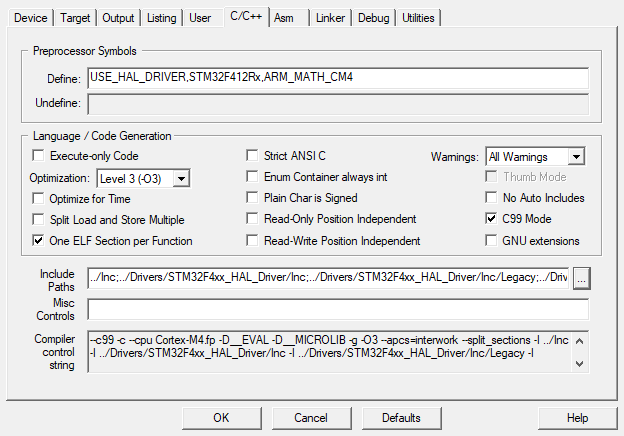
\includegraphics[width=1.0\linewidth]{Keil_Cmsis_Symbols}
	\caption{Options for Target 'P5 DSP Board'}
	\label{pic:Keil_Cmsis_Symbols}
\end{figure}

Des weiteren muss in den Projektoptionen die DSP Library zu den Include Paths hinzugefügt werden.

Unter \texttt{Project > Options for Target 'DSP Board' > C/C++ > Include Paths} muss der String \texttt{../Drivers/CMSIS/DSP/Include} hinzugefügt werden.

Weiterhin muss der CMSIS/DSP Mitgeteilt werden, welche CPU Architektur verwendet wird. Im Falle des \texttt{STM32F4xx} entspricht dies dem Wert \texttt{ARM\_MATH\_CM4}, der als Preprocessor Symbol im selben Konfigurationsfenster hinzugefügt werden muss.
Unter \texttt{Project > Options for Target 'DSP Board' > C/C++ > Preprocessor Symbols > Define:} muss der oben genannte String angefügt werden.





\todo{SB - Muss erklärt werden, wie dieses Package heruntergeladen wird? evtl. bei installation von Keil}


		\input{sections/4_2_4_DSPProcessing}
		\subsubsection{FIR Filter}
\label{sec:LibFIRFilter}

Als Wrapper für die CMSIS/DSP Funktionen für FIR Filter dienen die Dateien \texttt{fir.h} und \texttt{fir.c}. In dieser Library sind die Filterkoeffizienten in einem statischen Array abgelegt.


\paragraph{FIR Filter initialisieren}

Zusätzlich sind Init-Funktionen für das Mono- und Stereo-FIR Filter vorhanden. 
Das Initialisieren durch die Init Funktion muss vor dem Aufrufen der FIR-Processing Funktion geschehen, da die MCU sonst in einen Hard Fault läuft.

Im \texttt{main.c} muss der nachfolgende Code zur Initialisierung aufgeruffen werden.

\begin{lstlisting}[style=Cuvision, caption={Init Funktion der FIR Filter}]
/* USER CODE BEGIN 2 */
FIR_Init_Mono();
FIR_Init_Stereo();
/* USER CODE END 2 */
\end{lstlisting}


\paragraph{Filterkoeffizienten mit MATLAB berechnen}

Die Berechnung eines konkreten Filters ist nicht Teil dieses Projekts.
Für die Beispielimplementation des FIR Filters wurde für das Mono-Filter das Tiefpassfilter Example aus der CMSIS/DSP Dokumentation verwendet. 
Eine Kopie des Beispielcodes ist im Projekt unter \\
\texttt{./Drivers/CMSIS/DSP/Examples/ARM/arm\_fir\_example/arm\_fir\_example\_f32.c} enthalten.
Die Dokumentation des Filters bzw. der gesamten CMSIS/DSP Library ist auf der Webseite von ARM \cite{cmsis-doc-arm} oder Keil \cite{cmsis-doc-keil} abrufbar.

Für das Stereofilter wurde mit dem \texttt{fir1} MATLAB-Befehl die 11 Filterkoeffizienten berechnet. Das Filter hat eine 3dB-Grenzfrequenz bei $6/24 \pi rad/Sample$.

Die MATLAB-Funktion \texttt{fir1} arbeitet mit der \textit{Windowing-Methode} \cite{FIR-Windowing}, die nächer im Abschnitt \ref{sec:LibFIRAdaptive} beschrieben wird.
Dabei steht das erste Argument (hier: 10) für den Filtergrad oder $Anzahl Koeffizienten\ -\ 1$. Der zweite Parameter ist die auf die Samplingfrequenz normierte Grenzfrequenz.

\begin{lstlisting}[language=matlab]
fir1(10, 6/24)
\end{lstlisting}



		\subsubsection{FIR Filter mit anpassbarer Grenzfrequenz}
\label{sec:LibFIRAdaptive}

Damit auf dem STM32 dynamisch ein FIR Tiefpassfilter generiert werden kann, ist die Helperlibrary \texttt{adaptive\_fir.c} im Projektordner dabei.
Die Library enthält eine Funktion, die aus für eine gewünschte Grenzfrequenz die gewünschte Anzahl Koeffizienten liefert.
Dabei wird die \textit{Windowing-Methode} \cite{FIR-Windowing}, dessen Funktionsweise hier kurz erklärt wird, verwendet.
\\
\paragraph{Tiefpassfilter mit der Windowing Methode erzeugen}\vspace{-0.3cm}\\
Die Windowing Methode benutzt die Eigenschaft eines idealen Tiefpassfilters, dessen Amplitudengang einer $rect()$-Funktion (Abbildung \ref{pic:lowpass_ideal}) entspricht.
Wird $rect()$-Funktion Laplace-Transformiert, hat sie im Zeitbereich die Funktion $\frac{\sin{x}}{x}$ bzw. $sinc(x)$ - Abbildung \ref{pic:lowpass_sinc}.

\begin{figure}[H]
	\centering
	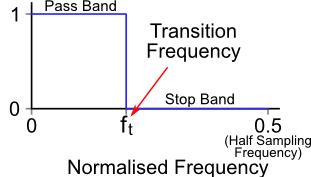
\includegraphics[width=0.4\linewidth]{lowpass_ideal}
	\caption{Amplitudengang eines idealen Tiefpassfilters mit Grenzfrequenz $f_t$ \cite{FIR-Windowing}}
	\label{pic:lowpass_ideal}
\end{figure}

\begin{figure}[H]
	\centering
	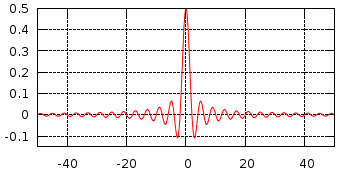
\includegraphics[width=0.4\linewidth]{lowpass_sinc}
	\caption{Die Impulsantwort eines idealen Tiefpassfilters folgt der Funktion $\frac{\sin{x}}{x}$ \cite{FIR-Windowing}}
	\label{pic:lowpass_sinc}
\end{figure}

Da die Funktion in Abbildung \ref{pic:lowpass_sinc} der Impulsantwort, und somit den Koeffizienten des Filters entspricht, lassen sich durch das Modellieren der $sinc()$-Funktion die Filterkoeffizienten berechnen.
Um das Filter zusätzlich zu verbessern, können die Koeffizienten optional mit einer der vielen Fensterfunktionen (Windows) gewichtet werden.
\\
\paragraph{Anwendung im C-Code}\vspace{-0.3cm}\\
In der Helperlibrary ist eine Funktion \texttt{fir1\_win} enthalten.
Die Parameter der Funktion sind ähnlich dem MATLAB-Befehlt \texttt{fir1}.
Im unten aufgeführten Listing ist gezeigt, wie die Funktion benutzt wird, um die Koeffizienten für ein Tiefpassfilter mit der Grenzfrequenz $f_g=1.0\si{kHz}$ bei einer Samplingrate von $f_s=48.0\si{kHz}$ zu erzeugen.\\

\begin{lstlisting}[style=Cuvision, caption={Berechnung von 19 Koeffizienten in C}]
uint8_t num_taps = 19;
float32_t new_coeffs[num_taps];
fir1(num_taps, 1000.0f/48000.0f, new_coeffs);
\end{lstlisting}


Nachfolgend der äquivalente MATLAB Befehl mit zusätzlichen Darstellungsformen.\\

\begin{lstlisting}[language=matlab, caption={Berechnung von 19 Koeffizienten in MATLAB}]
num_taps = 19;
new_coeffs = fir1(num_taps-1, 1000/48000)
% Koeffizienten darstellen
stem(new_coeffs)
grid on
% Uebertragungsfunktion anzeigen
freqz(new_coeffs)
\end{lstlisting}




\clearpage
	\subsection{Konfiguration mit STM32CubeMX}
\label{sec:CubeMX}

In den nachfolgenden Unterkapiteln sind die Konfigurationen in der STM32CubeMX Software abgebildet und beschrieben. Zudem sind Code Beispiele aufgeführt, die zeigen, wie die konfigurierte Peripherie im Projekt verwendet wird.

In der Abbildung \ref{pic:CubeMX_Pinout} ist das Pinout des STM32F412 ersichtlich.


\begin{figure}[H]
	\centering
	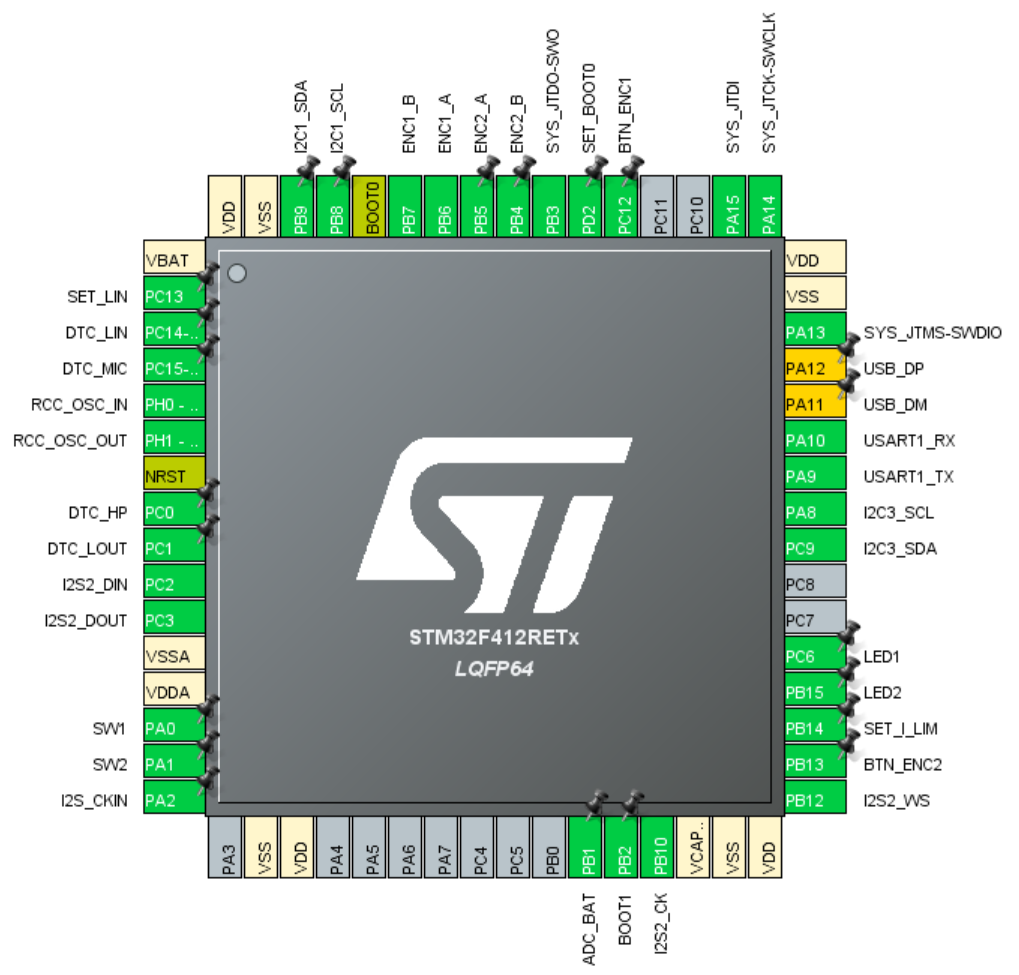
\includegraphics[width=0.9\linewidth]{CubeMX_Pinout}
	\caption{Pinout des STM32F412 in STM32CubeMX}
	\label{pic:CubeMX_Pinout}
\end{figure}





		\subsubsection{Encoder Mode mit Hardware Timer}
\label{sec:Conf_Encoder}

Einige integrierte Timer im STM32 unterstützen einen Encoder Modus, bei dem 2 vorgegebene GPIO
Pins den Zählstand des Timers verändern können.
In der Konfiguration wird die Zählrichtung mit Counter Mode auf \texttt{Up} gesetzt.
Der maximale Zählerwert (Periode) ist der Maximalwert eines \texttt{uint16\_t} Datentyps $P_{max}=2^{16}-1=65'535$.
In Abbildung \ref{pic:CubeMX_TIM3} ist die Konfiguration für den Timer 3 dargestellt. Der Timer 4 erhält die selbe Konfiguration.

\begin{figure}[H]
	\centering
	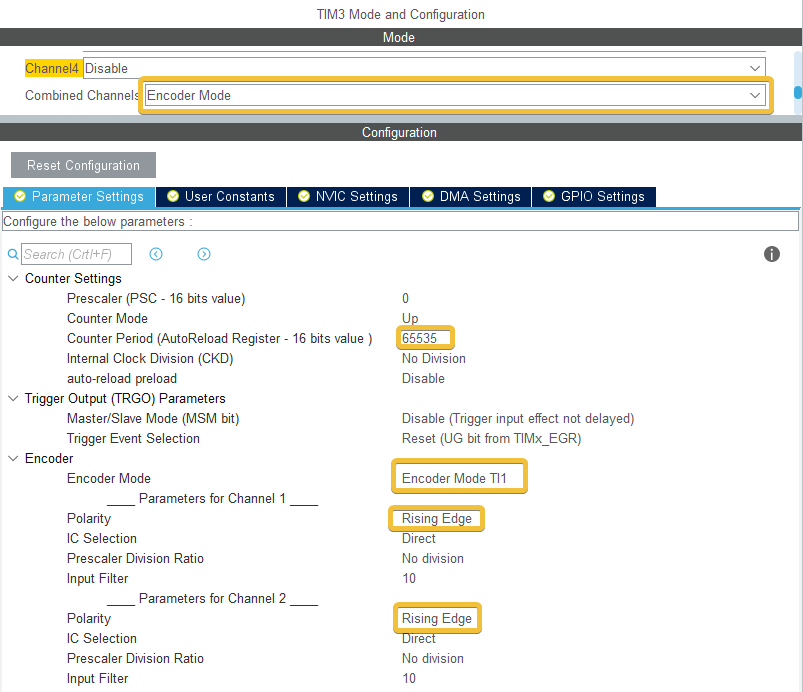
\includegraphics[width=0.9\linewidth]{CubeMX_TIM3}
	\caption{Konfiguration des Timer 3 im Encoder Modus}
	\label{pic:CubeMX_TIM3}
\end{figure}

\paragraph{Parameter}

Die nachfolgende Tabelle listet einige wichtige Parameter und deren Einfluss.

\begin{table}[H]
	\begin{tabular}{|l|l|l|}
		\hline
		\textbf{Setting} & \textbf{Werte} & \textbf{Erklärung}                            \\ \hline
		Counter Mode     & Up | Down      & Zählrichtung in Abhängigkeit der Drehrichung  \\ \hline
		Counter Period   &                & maximaler Zählerwert (z.b. uint16\_t)         \\ \hline
		Encoder Mode     & T1 | T2        & \begin{tabular}[c]{@{}l@{}}Triggerfokus auf CH1 oder CH2 oder beides.
			\\ Wenn beide aktiviert sind, zählt der Timer doppelt.\end{tabular} \\ \hline
	\end{tabular}
\end{table}

\paragraph{Anwendung im Code}

Das untenstehende Listing stellt dar, wie der Timer im \texttt{main.c} gestartet werden muss.
Eine Initialisierung alleine reicht nicht aus.

\begin{lstlisting}[language=c]
/* USER CODE BEGIN 2 */
// start Encoder mode on one channel
HAL_TIM_Encoder_Start(&htim2, TIM_CHANNEL_1);
/* USER CODE END 2 */
\end{lstlisting}

Mit dem unten gezeigten Befehl lässt sich der aktuelle Zählstand des Timers resp. Encoders auslesen.

\begin{lstlisting}[language=c]
/* USER CODE BEGIN x */
int new_encoder_val = TIM2->CNT;   // read encoder count anywhere in the code 
/* USER CODE END x */
\end{lstlisting}





		\subsubsection{Inter Integrated Sound (I\textsuperscript{2}S)}
\label{sec:CubeMXI2S}

Der STM32F412 verfügt über mehrere integrierte I\textsuperscript{2}S Interfaces. 
Für die Kommunikaiton mit dem TLV320 Codec wird Das I\textsuperscript{2}S2 Interface benutzt.
Nachfolgend wird die Konfiguration mit der STM32CubeMX beschrieben.
Die Abbildung \ref{pic:CubeMX_I2S} zeigt die wichtigsten Parameter für den Datenfluss.

\begin{figure}[H]
	\centering
	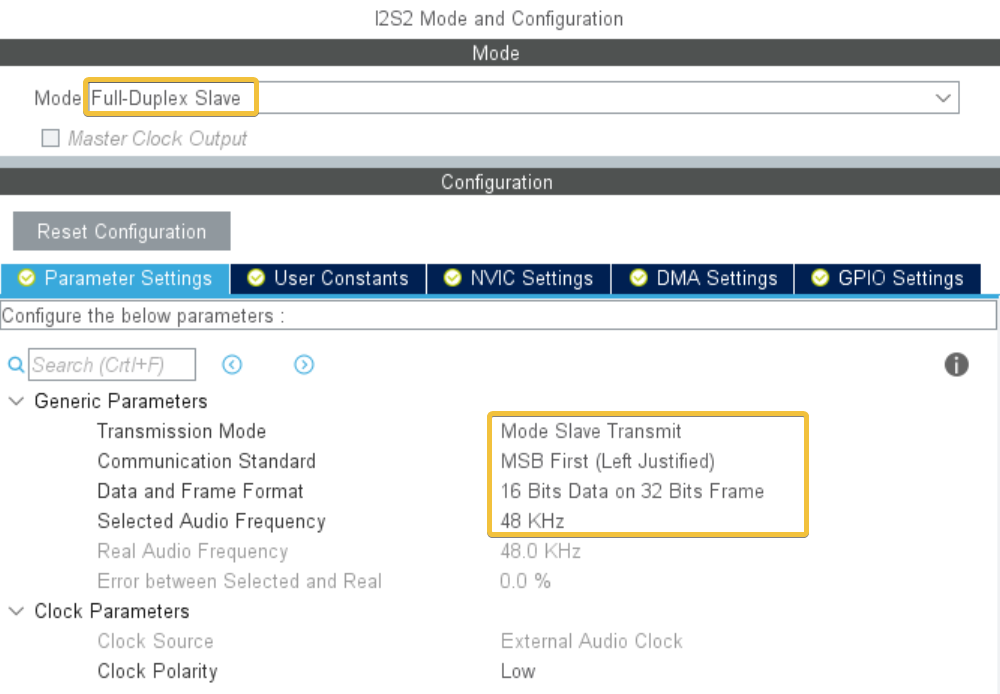
\includegraphics[width=0.9\linewidth]{CubeMX_I2S}
	\caption{Parameter Einstellungen der I\textsuperscript{2}S2 Schnittstelle}
	\label{pic:CubeMX_I2S}
\end{figure}

Da der TLV320 Codec im Master Modus betrieben wird, ist der STM32 im \\
\texttt{Mode Slave Transmit}.
Auch die Justification und die Wortbreite muss mit dem TLV320 übereinstimmen. Hier wird \texttt{MSB First} mit 16 Bits auf einem 32 Bit Frame eingestellt.
Die Samplingrate beträgt $f_s = 48\si{kHz}$.

Für die I\textsuperscript{2}S Schnittstelle wird die automatische Datenübertragung mittels DMA verwendet. Die Konfiguration des DMA Controllers ist in Abschnitt \ref{sec:CubeMXDMA} beschrieben.


		\subsubsection{Inter Integrated Circuit (I2C)}
\label{sec:CubeMXI2C}

Über insgesamt zwei I\textsuperscript{2}C Busse (I\textsuperscript{2}C1 / I\textsuperscript{2}C3) werden die beiden SSD1306 OLED Displays und der TLV320 angesprochen.
Beide Busse werden nach den Standardeinstellungen gemäss Abbildung \ref{pic:CubeMX_I2C1} betrieben.
Die Clock Frequenz beträgt $100\si{kHz}$, die Adressbreite 7 Bit.
Es werden keine Interrupts oder DMA verwendet.

\begin{figure}[H]
	\centering
	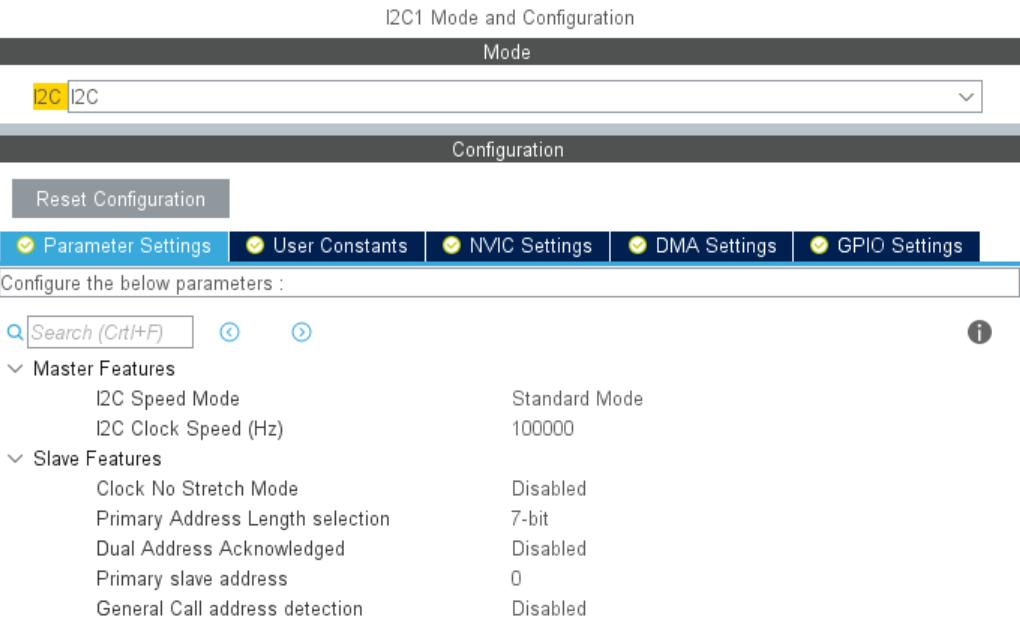
\includegraphics[width=0.9\linewidth]{CubeMX_I2C1}
	\caption{Parameter Einstellungen der I\textsuperscript{2}C1 und  I\textsuperscript{2}C3 Schnittstelle}
	\label{pic:CubeMX_I2C1}
\end{figure}





		\subsubsection{Asynchron UART (Debug Interface)}
\label{sec:CubeMXUart}

Auf dem DSP Board sind die beiden Pins \texttt{PA9 (Rx)} und \texttt{PA10 (Rx)} auf Testpoints geführt. 
Über die UART Schnittstelle \texttt{USART1} kann ein Serieller Adapter angeschlossen werden.
Die Abbildung \ref{pic:CubeMX_Uart} zeigt die Standardeinstellungen mit einer Baudrate von $115200 \si{Bd}$. Interrupts oder DMA werden nicht verwendet.

\begin{figure}[H]
	\centering
	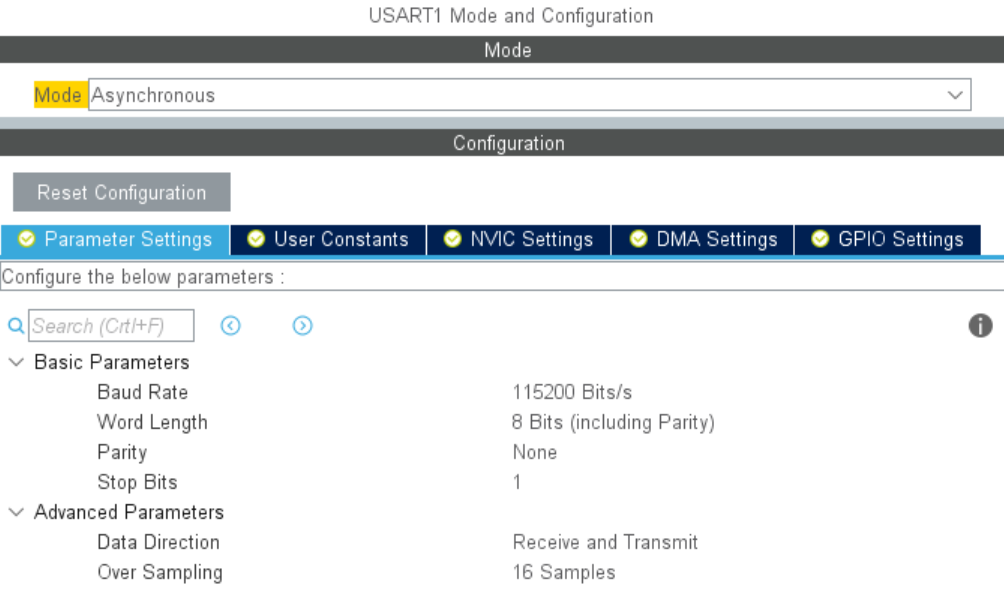
\includegraphics[width=0.9\linewidth]{CubeMX_Uart}
	\caption{Parameter Einstellungen der USART1 Schnittstelle}
	\label{pic:CubeMX_Uart}
\end{figure}

		\subsubsection{Analog Input GPIO (ADC)}
\label{sec:CubeMXADC}



		\subsubsection{Direct Memory Access (DMA)}
\label{sec:CubeMXDMA}

Die I\textsuperscript{2}S Schnittstellen unterstützen den automatischen Datentransfer über den DMA Controller. In der Abbildung \ref{pic:CubeMX_I2S_DMA} ist die Konfiguration für den Peripheral to Memory Kanal ersichtlich. Der Memory to Peripheral Kanal wird mit den selben Einstellungen konfiguriert. \texttt{Half Word} bedeutet eine Datenbreite von 16 Bit, was der bei der I\textsuperscript{2}S2 Schnittstelle (Abschnitt \ref{sec:CubeMXI2S}) eingestellten Datenwortbreite entspricht.

\begin{figure}[H]
	\centering
	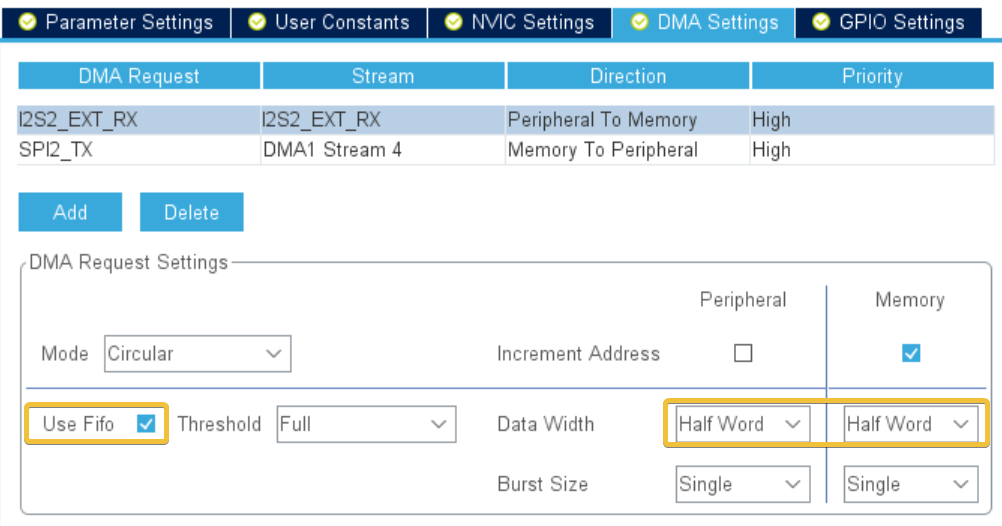
\includegraphics[width=0.9\linewidth]{CubeMX_I2S_DMA}
	\caption{DMA Einstellungen der I\textsuperscript{2}S2 Schnittstelle}
	\label{pic:CubeMX_I2S_DMA}
\end{figure}


		\subsubsection{Interrupt Funktionen (NVIC)}
\label{sec:CubeMXNVIC}



		\subsubsection{Clock Konfiguration}
\label{sec:CubeMXClock}

Der STM32F412 hat einen $f_{HSE}=8.000\si{MHz}$ Clock von einem Quarz Oszillator.
Dazu muss unter \texttt{System Core > RCC} die High Speed Clock (HSE) auf \texttt{Crystal/Ceramic Resonator} gesetzt werden. Die Abbildung \ref{pic:CubeMX_RCC} zeigt die notwendigen Einstellungen.

Da der TLV320 im Master Mode betrieben wird, kommt auch der Clock für die I\textsuperscript{2}S Peripherie vom TLV320 über den \texttt{CLK\_OUT} Pin.
Die I\textsuperscript{2}S Clock Frequenz beträgt $f_{clk}=12.288\si{MHz}$.
Im \texttt{RCC} Reiter muss die Audio Clock Input (\texttt{I2S\_CKIN}) aktiviert werden.

\begin{figure}[H]
	\centering
	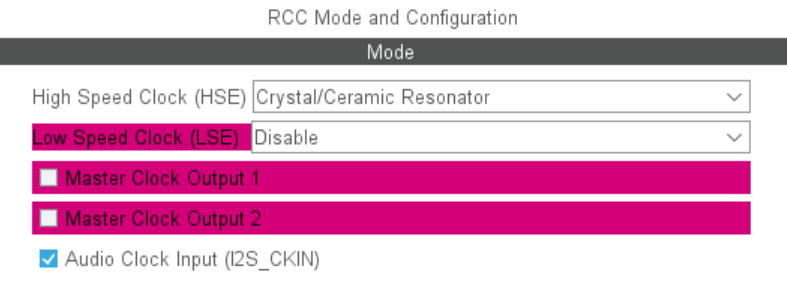
\includegraphics[width=0.6\linewidth]{CubeMX_RCC}
	\caption{Auswahl der externen Clock (HSE)}
	\label{pic:CubeMX_RCC}
\end{figure}

Die maximale Taktfrequenz des STM32F412 liegt bei $f_{CPU}=100\si{MHz}$.
Damit die Geschwindigkeit erreicht wird, wird der interne PLL so konfiguriert, dass die CPU die maximale Taktfrequenz zugewiesen bekommt. Die Abbildung \ref{pic:CubeMX_Clock} zeigt alle notwendigen Konfigurationen inklusive der externen I\textsuperscript{2}S Clock.

\begin{figure}[H]
	\centering
	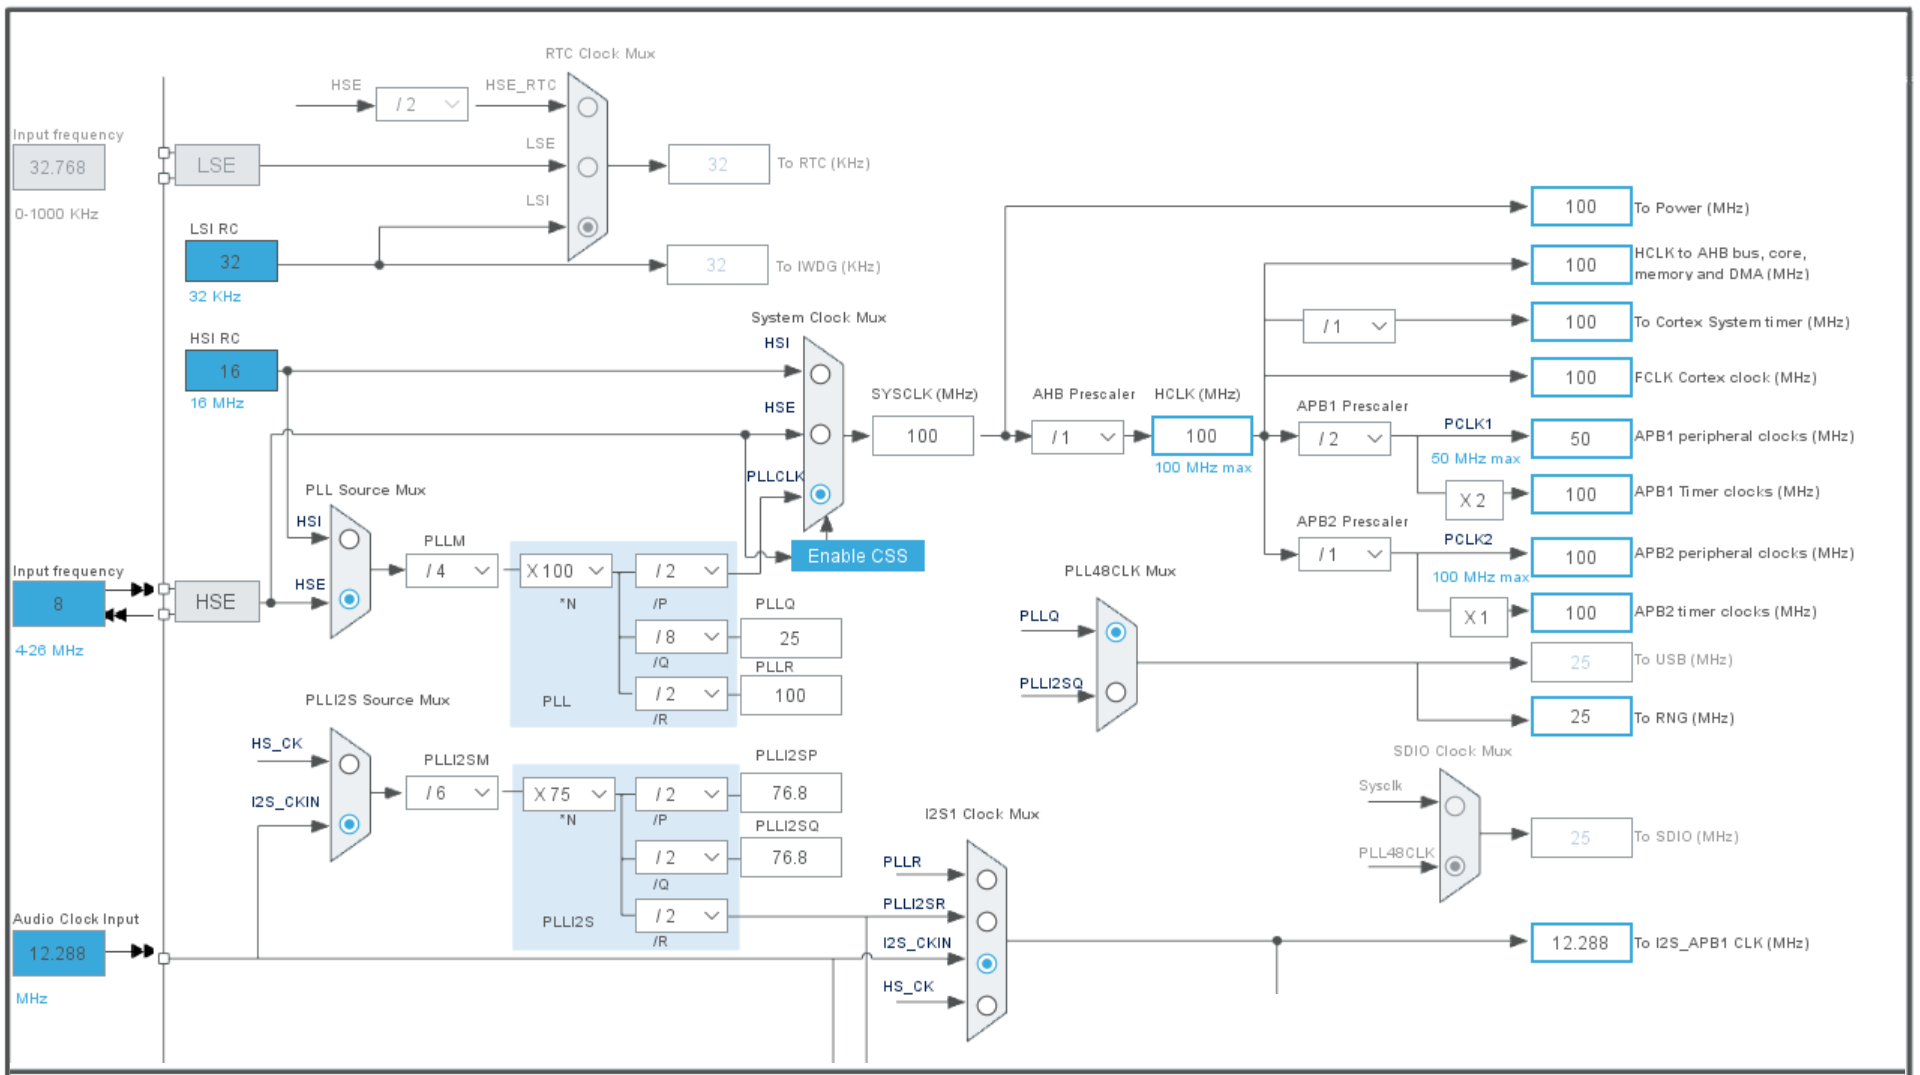
\includegraphics[width=1.0\linewidth]{CubeMX_Clock}
	\caption{Gesamtübersicht der Clockkonfiguration mit $f_{CPU}=100\si{MHz}$}
	\label{pic:CubeMX_Clock}
\end{figure}

\newpage
\clearpage
	\subsection{Digitaler Datenfluss}
\label{sec:DSPKonzept}

In diesem Abschnitt wird gezeigt, wie der Datenstrom vom Codec über den DMA-Controller des STM32,
durch die CMSIS/DSP Library und zurück über den DMA-Controller zum Codec gelangt.
Dabei werden die wichtigen Programmierschnittstellen und Konfigurationen hervorgehoben.

\todo{SB}





		\subsubsection{Digitaler Datenfluss}
\label{sec:Dataformat}

Nachfolgend wird zuerst dargestellt, wie der Datenfluss vom und zum Codec aussieht und zu interpretieren bzw. verarbeiten ist. 
Sowohl der STM32 als auch der Codec unterstützen weitere Betriebsmodi (Left/Right Justified, MSB/LSB First). Hier ist nur die implementierte Variante beschrieben.

Die Abbildung \ref{pic:I2S_Datastream} zeigt einen Datenfluss, wie er aus dem Codec über die \texttt{I2S\_DOUT} Leitung heraus kommt. 
Das verwendete Datenformat ist \textit{16 Bit Data Word on a 32 Bit Frame}. Das bedeutet, dass der Samplingwert 16 Bit gross (\texttt{int16\_t}) ist, und von 16 weiteren Leerbits begleitet wird.
Der Datenfluss ist \textit{Left Justified}, was bedeutet, dass pro Abtastwert immer zuerst der linke Kanal gefolgt vom rechten Kanal übertragen wird.

\begin{figure}[H]
	\centering
	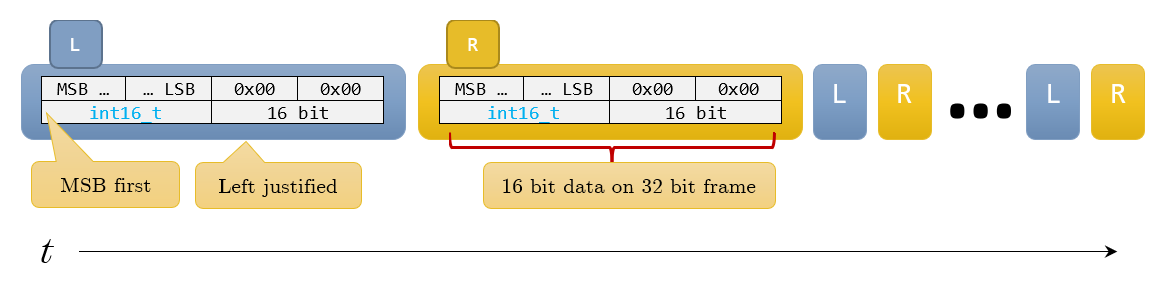
\includegraphics[width=1.0\linewidth]{I2S_Datastream}
	\caption{Zeitliche Abfolge der Samplingwerte vom und zum Codec}
	\label{pic:I2S_Datastream}
\end{figure}

Damit der Datenstrom richtig empfangen wird, ist die I\textsuperscript{2}S Schnittstelle entsprechend Konfiguriert, siehe Abschnitt \ref{sec:CubeMXI2S}.
Um die Daten automatisch im RAM des STM32F412 abzuspeichern, kommt der DMA Controller zum Einsatz, dessen Konfiguration in Abschnitt \ref{sec:CubeMXDMA} beschrieben ist.

\begin{figure}[H]
	\centering
	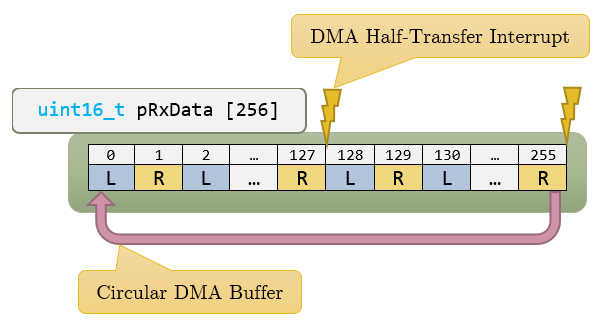
\includegraphics[width=0.6\linewidth]{DMA_CircularBuffer}
	\caption{Aufbau des Circular Buffers der beim DMA verwendet wird.}
	\label{pic:DMA_CircularBuffer}
\end{figure}

Der DMA Controller schreibt die Daten kontinuierlich in ein \texttt{uint16\_t} Array der Länge 256. Im \textit{Circular Buffer} Modus, wird beim Erreichen des Bufferende der DMA Pointer automatisch wieder an den Anfang gesetzt, siehe Abbildung \ref{pic:DMA_CircularBuffer}.
Mit der passenden Interrupt Konfiguration wird immer bei halbem und vollem Füllstand des Buffers ein \textit{DMA Half-Transfer Interrupt} ausgelöst.
So kann jeweils die Hälfte des zuvor geschriebenen Buffers verarbeitet werden.




		\subsubsection{Digitaler Datenfluss}
\label{sec:Dataflow}

Die Abbildung \ref{pic:DMA_Dataflow} zeigt den Datenfluss durch den STM32 mit den jeweils verwendeten Datentypen, den Routinen und den Quelldateien.

\begin{figure}[H]
	\centering
	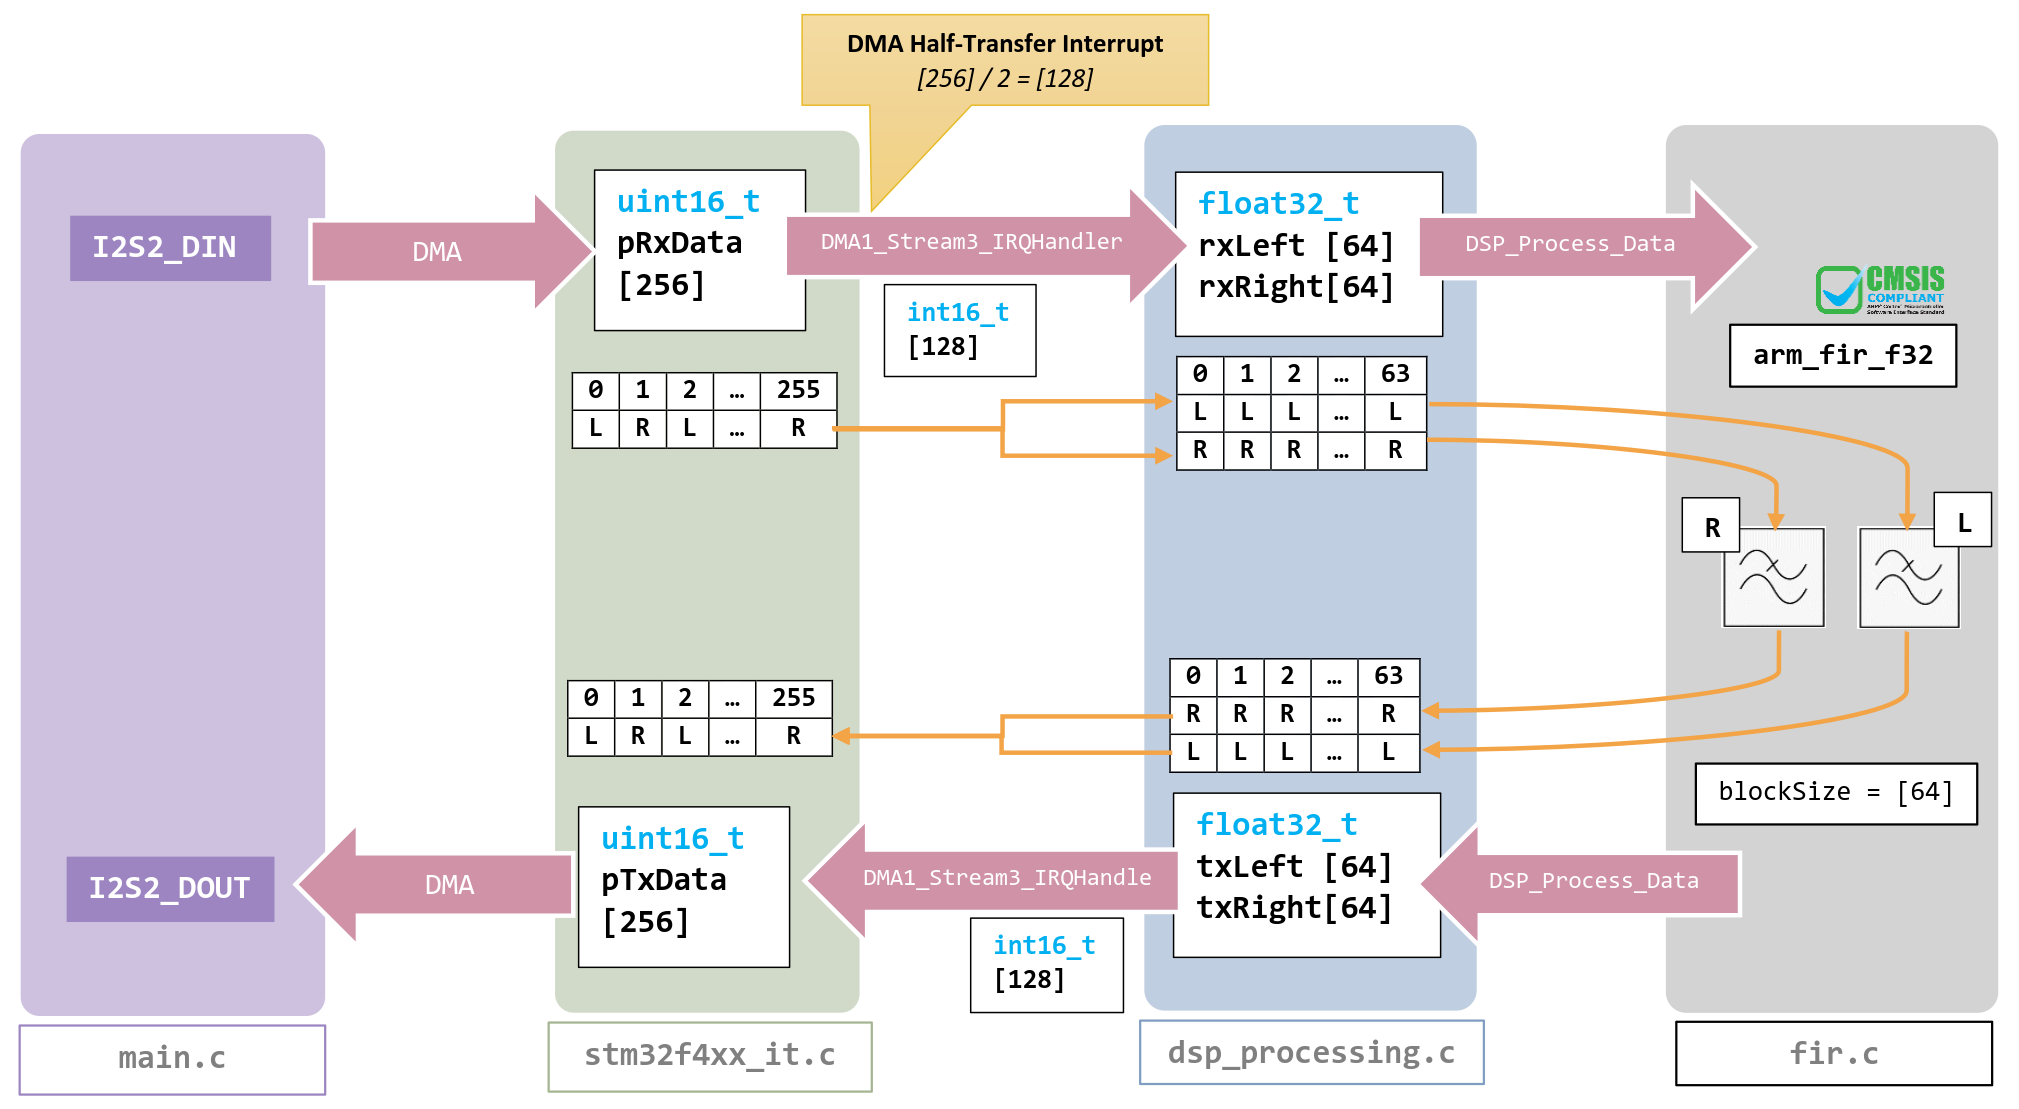
\includegraphics[width=1.0\linewidth]{DMA_Dataflow}
	\caption{Signalfluss des abgetasteten Audiosignals durch die verschiedenen Stufen der Verarbeitung}
	\label{pic:DMA_Dataflow}
\end{figure}

 Die Datenverarbeitung läuft folgendermassen ab:\\

Der DMA Controller wird im \texttt{main.c} so gestartet, dass ankommende Daten automatisch in den \texttt{uint16\_t} Buffer \texttt{pRxData} geschrieben werden. Die Datengrösse des DMA Buffers ist 256. 

Sobald der Buffer halb voll (128 Samples) ist, wird ein DMA Half-Transfer Interrupt ausgelöst.
Dieser Interrupt wird im der ISR \texttt{DMA1\_Stream3\_IRQHandler()} abgearbeitet. 
In der ISR werden die neuen gültigen Daten der Länge 128 an die Routine \texttt{DSP\_Process\_Data} übergeben, die die \texttt{uint16\_t} Werte explizit zu \texttt{int16\_t} castet. Ein Cast auf Signed ist notwendig, da das Audiosignal als signed zu interpretieren ist. Anschliessend folgt ein impliziter Cast auf \texttt{float32\_t}.

Bei der Wandlung auf \texttt{float32\_t} wird der Audiostream auf den linken und rechten Kanal in zwei Buffer \texttt{rxLeft} und \texttt{rxRight} aufgesplittet.
So stehen diese für die weitere Verarbeitung zur Verfügung durch verschiedene DSP Funktionen zur Verfügung.
Die beiden float-Buffer werden nun an die FIR Filterfunktion \texttt{FIR\_Filter\_F32\_Stereo} überreicht. In dieser Funktion wird ein zuvor initialisiertes FIR Filter aus der CMSIS/DSP Library ausgeführt.
Der Rückgabewert wird in den beiden Outputbuffern \texttt{txLeft} und \texttt{txRight} gespeichert.

Anschliessend folgt das Casting zurück zu \texttt{uint16\_t}. Bei diesem Schritt werden die Samples wieder auf die Anfangsreihenfolge mit abwechselnd linkem und rechtem Samplewert verteilt.
Der DMA Controller ist bereits im \texttt{main.c} so konfiguriert, diesen Outputbuffer \texttt{pTxData} automatisch über die \texttt{I2S2} Peripherie zu senden.

\begin{table}[H]
	\centering
	\begin{tabular}{|l|r|l|}
		\hline
		\textbf{\#define}       & \textbf{Wert} & \textbf{Beschreibung}                                                 \\ \hline
		\texttt{DSP\_BUFFERSIZE} & 128 & Anzahl Samples (L+R) pro DMA Interruptzyklus \\ \hline
		\texttt{DSP\_BUFFERSIZE\_HALF} & 64 & \begin{tabular}[c]{@{}l@{}}Anzahl Samples pro Kanal.\\ Auch blockSize für FIR Filter\end{tabular} \\ \hline
	\texttt{	DSP\_BUFFERSIZE\_DOUBLE} & 256 & Grösse des Circular Buffers für den I2S DMA \\ \hline  
	\end{tabular}
	\caption{Erklärung der Werte im C-Code}
	\label{tab:buffer_sizes}
\end{table}

Die Tabelle \ref{tab:buffer_sizes} stellt den Bezug zu der Abbildung \ref{pic:DMA_Dataflow} und dem C-Code her. 


		\subsubsection{Konzept zur Verkettung von Effekten}
\label{sec:DSPChaining}

In einem nachfolgenden Schritt, soll die Software in der Lage sein, mehrere DSP Effekte hinter einander zu schalten. Nachfolgend ist ein Konzept beschrieben, wie die DSP Daten von Block zu Block weitergereicht werden können.

\begin{figure}[H]
	\centering
	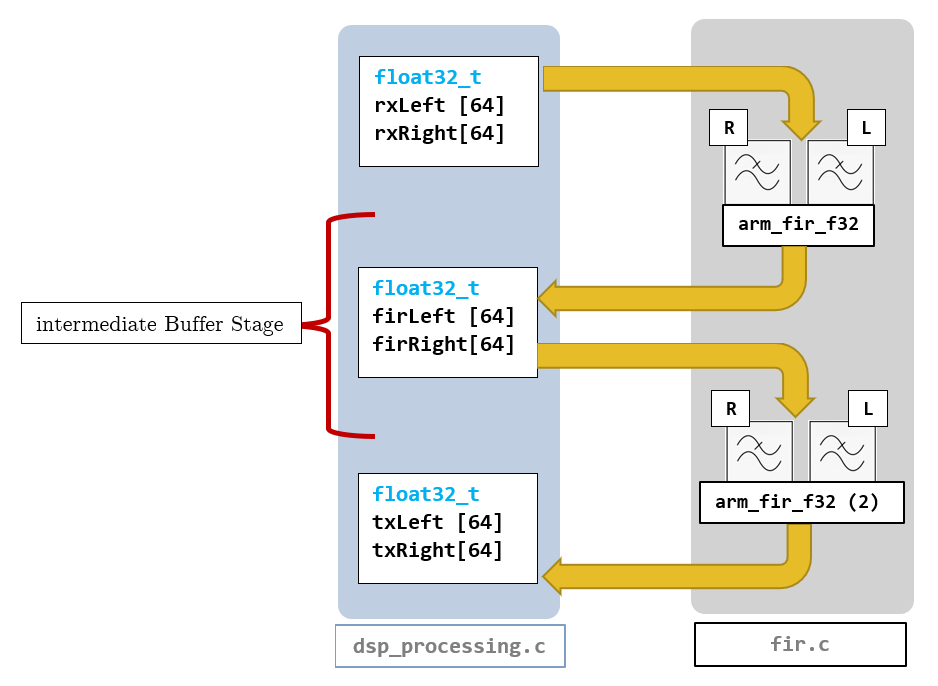
\includegraphics[width=0.8\linewidth]{Buffer_stage}
	\caption{Mögliche Erweiterung der FIR Funktion aus dem \texttt{dsp\_processing.c} durch Verwendung eines dazwischenliegenden Buffers.}
	\label{pic:Buffer_stage}
\end{figure}

Die Abbildung \ref{pic:Buffer_stage} zeigt die letzten beiden Abschnitte der Datenverarbeitung. Die Datei \texttt{fir.c} bleibt unverändert und enthält weiterhin nur FIR Filter. An ihrer Stelle könnte auch eine andere Datei mit anderen DSP Funktionen stehen.
Die Daten werden in Form eines Buffers an die nächste Funktion weitergereicht.
Damit die Datenverarbeitung wie gewünscht funktioniert, muss im \texttt{dsp\_processing.c} das Management der Buffer im Sinne von "\textit{Verbindungskabel}" verwaltet werden.

Das nachfolgende Listing zeigt das Beispiel aus Abbildung \ref{pic:Buffer_stage}, bei dem die Daten durch zwei FIR Filter durchgereicht werden.

\begin{lstlisting}[style=Cuvision, caption={Daten mittels Buffer und zwei FIR Filter bearbeiten}]
// process rxLeft in FIR(1), store in intermediate buffer: firLeft
arm_fir_f32(&FIR_F32_Struct_1, rxLeft, firLeft, blockSize);
// process firLeft in FIR(2), output to txLeft
arm_fir_f32(&FIR_F32_Struct_2, firLeft, txLeft, blockSize);

\end{lstlisting}

Dieses Konzept weist folgende drei Punkte auf, die beim Design beachtet werden müssen.
Einerseits nimmt mit jedem Buffer dazwischen die \textbf{Latenzzeit} um $t_{lat}=BUFFERSIZE*t_S=64*\frac{1}{48'000\si{Hz}}=1.3\si{ms}$ zu.
Weiterhin steigt mit der Anzahl Buffer auch der \textbf{RAM Bedarf} um $BUFFERSIZE*n_{Bytes}*n_{channels}=64*2*2=256\si{Bytes}$ pro Buffer.
Zuletzt steigt mit jedem neuen Effekt auch die \textbf{Rechenzeit}. Diese muss in jedem Fall individuell beachtet werden, da sie auch stark von der Art des Effektes abhängt.
Die gesamte Rechenzeit darf auf keinen Fall länger als die oben berechneten $1.3\si{ms}$, die der zeitlichen Länge eines Buffers beträgt, sein.




\clearpage
	\subsection{Programmierung über USB mit Device Firmware Upgrade (DFU) Modus}
\label{sec:USBDFU}

Dieses Kapitel beschreibt, wie die Firmware auf dem STM32 ohne Debugger über USB programmiert werden kann.

Von STM32 wird die sogenannte DfuSe Demosoftware mit entsprechender Dokumentation geliefert. 
Der Hersteller STMicroelectronics zeigt mit der Software, wie man die Firmware-Upgradefunktion in eigene Software integrieren kann.



		\subsubsection{Bootloader starten}
\label{sec:Enter_DFU}

Der STM32 muss in den internen Bootloader starten. Dies könnte theoretisch über Software (Assembler) per Anpassung der \texttt{startup.s} Datei erreicht werden.
Jedoch ist auf dem DSP Board eine Schaltung vorhanden, um den \texttt{BOOT0} Pin vorübergehend auf \texttt{HIGH} zu ziehen.
Wenn ein Starten des Bootloaders und somit des DFU Modus gewünscht wird, muss dies in der Software folgendermassen realisiert werden.
\\
\begin{lstlisting}[style=Cuvision,caption={Starten des Bootloaders durch CPU Reset}]
/* If User Button is pressed on Startup, enter DFU Firmware Upgrade Mode */
if(HAL_GPIO_ReadPin(SW2_GPIO_Port, SW2_Pin) == GPIO_PIN_SET){
  // pull BOOT0 = 1
  HAL_GPIO_WritePin(SET_BOOT0_GPIO_Port, SET_BOOT0_Pin, GPIO_PIN_SET);
  HAL_Delay(500);      // wait for Capacitor to charge to ~3.3V
  NVIC_SystemReset();  // Reset the MCU
}
\end{lstlisting}

Das oben aufgeführte Listing beschreibt das Auslösen des DFU Modus sobald der einer der User Buttons gedrückt wird.
Damit der Kondensator Zeit hat, sich aufzuladen, wird ein Delay von ca. 500ms benötigt.
Anschliessend wird mit dem Befehl \texttt{NVIC\_SystemReset()} ein Software Reset ausgelöst.
Der STM32 sollte nun in den Bootloader starten.

Vor dem Systemreset besteht die Möglichkeit, einen Hinweisstring (z.B. \textit{\glqq upgrading...\grqq}) auf dem OLED Display anzuzeigen.
Der Text bleibt während dem Upgrade bestehen, da die Spannungsversorgung nicht unterbrochen wird.




		\subsubsection{DfuSe Programm}
\label{sec:DFUSe}

STMicroelectronics stellt eine Software namens DfuSe zur Verfügung um die Firmware STM32 Devices ohne Debugger zu programmieren. Siehe Kapitel \ref{sec:KeilInstall} für die Installation des DfuSe Tools.

\paragraph{HEX File zu DFU File konvertieren}

Für den Prozess verlangt das Tool, ein \texttt{.dfu} Dateiformat, dass nicht von der IDE erzeugt wird. 
Im Normalfall ist die kompilierte Binärdatei aus Keil uVision 5 im \texttt{.hex} Format im Projektordner unter \texttt{./MDK-ARM/<Projektname>/<Projektname>.hex} zu finden.\\

Das DfuSe Tool kommt mit einem weiteren Werkzeug, um Dateien vom \texttt{.hex} ins \texttt{.dfu} Format zu konvertieren. 
Dieses heisst DFU File Manager und ist in Abbildung \ref{pic:DFU_file_man} dargestellt.

\begin{figure}[H]
	\centering
	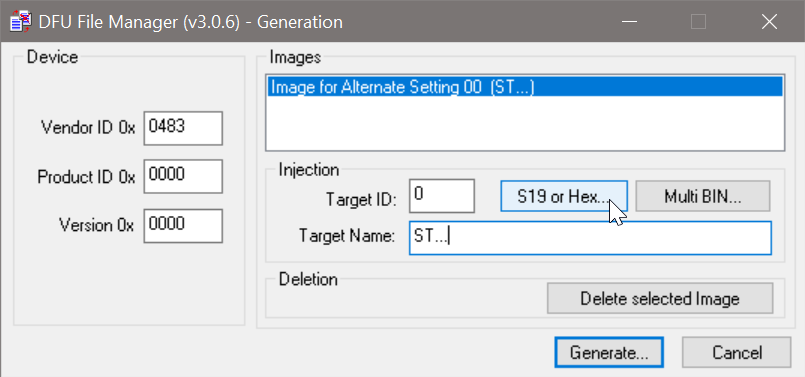
\includegraphics[width=0.5\linewidth]{DFU_file_man}
	\caption{Firmware Upgrade Tool DfuSe}
	\label{pic:DFU_file_man}
\end{figure}

Den DFU File Manager starten und \glqq\textit{I want to GENERATE a DFU file from HEX}\grqq \ auswählen.
Darauf präsentiert sich das Tool wie in Abbildung \ref{pic:DFU_file_man}. Hier kann eine \texttt{.hex} Datei ausgewählt und anschliessend konvertiert und gespeichert werden.
Mit Klick auf \textit{\glqq S19 or HEX...\grqq} kann das \texttt{<Projektname>.hex} ausgewählt und anschliessend mit Klick auf \textit{\glqq Generate...\grqq} ein \texttt{<Projektname>.dfu} generiert werden.
\\
\paragraph{DFU Datei auf das DSP Board laden}\vspace{-0.3cm}\\
Die nun erstellte \texttt{<Projektname>.dfu} Datei kann mit dem DfuSe Programm auf das im DFU Modus gebootete DSP-Board programmiert werden. 
Die Abbildung \ref{pic:DFUSe_Upgrade} zeigt das DfuSe Programm, bei dem das DSP-Board bereits am USB Port erkannt wurde. Die Erkennung geschieht automatisch, sofern das DSP-Board über USB am Computer angeschlossen ist und sich im Bootloader befindet.

\begin{figure}[H]
	\centering
	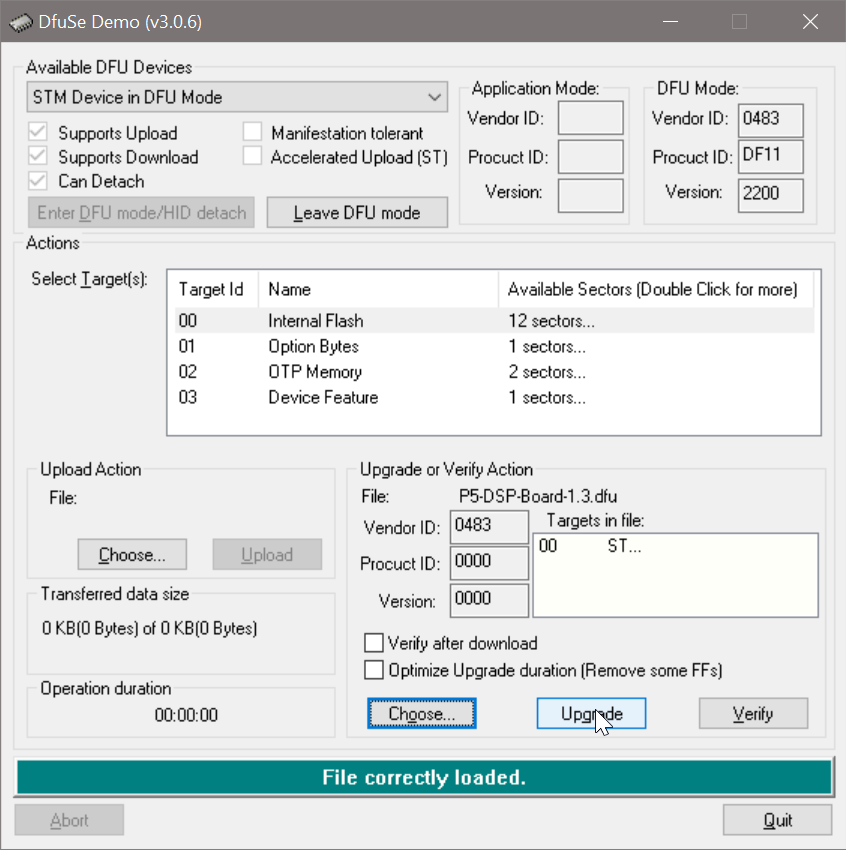
\includegraphics[width=0.65\linewidth]{DFUSe_Upgrade}
	\caption{Firmware Upgrade Tool DfuSe}
	\label{pic:DFUSe_Upgrade}
\end{figure}

Mit Klick auf \textit{\glqq Choose...\grqq} wird die \texttt{<Projektname>.dfu} ausgewählt.
Anschliessend mit \glqq\textit{Upgrade}\grqq die neue Firmware programmieren.
Dabei erscheint eine Warnung \textit{\glqq ...it is impossible to make sure this file is for device.\grqq}, welche mit \textit{\glqq Yes\grqq} bestätigt werden kann.

Wenn das Upgrade vollzogen ist, erscheint der Balken unten in grün. Jetzt kann das DSP-Board mit \textit{\glqq Leave DFU Mode\grqq} neu gestartet werden.



\clearpage
\section{Validierung}
\label{sec:Validierung}

Um die entworfene Schaltung und deren korrekte Funktion zu validieren, werden verschiedene Messungen mit einzelnen Teil-Schaltungen durchgeführt und interpretiert.
	\subsection{Spannungsversorgung}
\label{sec:Valid_Speisung}

Der Stromverbrauch beträgt 64mA

Kein Audio, beide Displays mit Menutext.

Vin 3.7 .. 4.2V

Messgerät SMU
Agilent N6705B		Channel 1	Strombegrenzung 600mA			PrüfmittelNr. MSZ-M-0064


	\subsection{Akkumulator}
\label{sec:Valid_Batterie}

\subsubsection{ADC Messung der Batteriespannung}

Die Spannungsmessung inkl. Korrekturfaktor für den Spannungsteiler mit Hilfe einer Source Measuring Unit überprüft. Die Dabei entstandenen Werte sind in der Abbildung \ref{pic:ADC_Spannung_Graph} geplottet.

\begin{figure}[H]
	\centering
	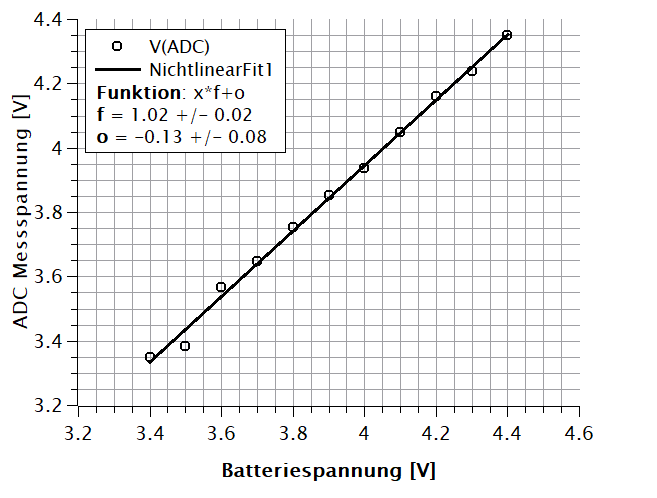
\includegraphics[width=0.8\linewidth]{ADC_Spannung_Graph}
	\caption{Akkumulatorspannung im Vergleich mit der gemessenen Spannung am ADC}
	\label{pic:ADC_Spannung_Graph}
\end{figure}

Auf die gemessenen Werte liefert ein linearer Fit folgende Erkenntnis.
Die Messwerte sind durchschnittlich um $V_{offset}=-130\si{mV}$ zu gering.
Zu einem Teil sind die Abweichungen auf die Widerstandtoleranzen des Spannungsteilers zurückzuführen.
Ein weiterer Einflussfaktor hat die Batteriespannung selber, da diese durch den BQ2409x nicht konstant gehalten wird. Auch das Fehlen einer Filterschaltung für das ADC Signal verschlechtert die Messergebnisse.

Verwendetes Messgerät:

Agilent N6705B (Prüfmittel Nr. \texttt{MSZ-M-0064}) auf Channel 1 mit Strombegrenzung $I_{max}=600\si{mA}$.

\todo{SB - Verweis auf einen Zielwert. zb. Eingehalten auf +- 100mV genau blabla reicht um Low Voltage zu detektieren}

\todo{SB - Ladestrom = 317mA ...}


	\subsection{Ressourcenbedarf und Timing der CMSIS/DSP Funktionen}
\label{sec:DSP_Timing}

Um den Ressourcenbedarf (Timing) besser abschätzen zu können, sind hier sind die Resultate einiger Performancetests aufgeführt.
Die Tests sind mit der im Abschnitt \ref{sec:Dataflow} beschriebenen Datenverarbeitungsstruktur durchgeführt worden.
Die Taktfrequenz des Cores beträgt $f_{CPU}=100\si{MHz}$.

Als Messmethode dient ein GPIO-Pin (LED\_1), der jeweils vor der Bearbeitung durch das FIR-Filter eingeschaltet und nach Beenden ausgeschaltet wird. 
Die Abbildung \ref{pic:FIR_Delay_Blocksize} zeigt, eine ganze Bearbeitungsperiode von $t_p=1.330\si{ms}$.
Diese Zeit kommt durch die Buffergrösse und die Abtastfrequenz zustande.
Da die Verarbeitung innerhalb einer Bufferlänge abgeschlossen sein muss, darf die 
kritische Zeit $t_p$ auf keinen Fall erreicht, oder überschritten werden.

\begin{equation}
	t_p=\frac{DSP\_BUFFER\_SIZE\_HALF}{f_s}=\frac{64}{48'000\si{Hz}}=1.333\si{ms}
\end{equation}


\subsubsection{Delay des Audio Passthrough}

Auch wenn die Daten beim Passthrough durch kein Filter geführt werden, wird beim Splitten des DMA Buffers in die beiden Kanalbuffer (L/R) Zeit benötigt.
Bei der Messung wird der GPIO vor dem Kopieren der Buffer eingeschaltet und danach wieder ausgeschaltet.

\begin{figure}[H]
	\centering
	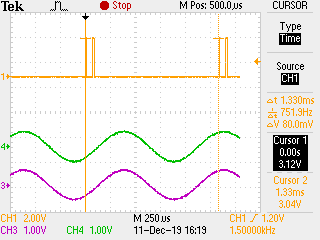
\includegraphics[width=0.6\linewidth]{FIR_Delay_Blocksize}
	\caption{Pulse zur Zeitmessung der Verarbeitungszeit. Die kleinen Pulse sind die Zeit zum Kopieren der rx-/tx-Buffer. Die kurze Lücke zwischen den Pulsen ist die Zeit für die Verarbeitung von zwei FIR Filtern mit je 11 Koeffizienten. Ausgangssignal L/R (grün/rot) 1kHz.}
	\label{pic:FIR_Delay_Blocksize}
\end{figure}

Die beiden kurzen Pulse in der Abbildung \ref{pic:FIR_Delay_Blocksize} entstehen durch den nachfolgend gelisteten Code in der Datei \texttt{dsp\_processing.c}.
Das Kopieren (Aufteilen in Links/Rechts) geschieht je ein Mal für die rxBuffer und die txBuffer, wobei ein Delay von $t_{Buffersplit}=16\mu\si{s}$ pro Kopiervorgang entsteht.
Die Abbildung \ref{pic:FIR_Delay_Blocksize} zeigt die Audiofunktion mit FIR-Filter. Im Falle der Verwendung einer Audio Passthrough Funktion beträgt die gesammte Verarbeitungszeit
inkl. Kopieren: $t_{delay}=40.8\mu\si{s}$. Daraus lässt sich schliessen, dass das Kopieren 
von rx in tx ohne weitere Verarbeitung nochmals ca. $f_{copy}=8\mu\si{s}$ benötigt.\\

\begin{lstlisting}[style=Cuvision, caption={GPIO togglen um die Kopierzeit zu messen}]
/* This Code takes 16 us for DSP_BUFFERSIZE_HALF = 64 and fCPU = 100MHz */
// copy sourceBuffer to leftSignalBuffer and rightSignalBuffer

HAL_GPIO_WritePin(LED1_GPIO_Port, LED1_Pin, GPIO_PIN_SET);

for (uint16_t index1 = 0; index1 < DSP_BUFFERSIZE_HALF; index1++) {
  rxLeft [index1] = (int16_t)(sourceBuffer[2*index1  ]);  
  rxRight[index1] = (int16_t)(sourceBuffer[2*index1+1]); 
}

HAL_GPIO_WritePin(LED1_GPIO_Port, LED1_Pin, GPIO_PIN_RESET);
\end{lstlisting}


\subsubsection{FIR Filter unterschiedlicher Anzahl Koeffizienten}

Theoretisch wird von einer FPU erwartet, dass diese ein FIR Filter mit der Effizienz von $1\frac{cycle}{TAP}$ mit Hilfe des Multiply-Accumulate Befehls (\texttt{MAC})) berechnet.
Bei ARM Cortex-M4 ist es jedoch so, dass das FIR Filter ohne Multiply-Accumulate Funktion kompiliert wird. Die Instruktion \texttt{VMLA.F32} benötigt 3 clock cycles \cite{ARM-M4-FPU-reference}. \\

\begin{lstlisting}[style=Cuvision,caption={Kompilierte Multiply-Accumulate Instruktion}]
0x080008E8 EE628A0D VMUL.F32 s17,s4,s26
0x080008EC EE766AA8 VADD.F32 s13,s13,s17
\end{lstlisting}

\begin{lstlisting}[style=Cuvision,caption={Multiply-Accumulate Befehl in C aus der CMSIS/DSP Library \texttt{arm\_fir\_f32.c}}, firstnumber=465]
    acc3 += x4 * c0;
\end{lstlisting}

Die folgende Messung liefert das tatsächliche Ergebnis.

Mit dem Nachfolgenden Code wird die Verzögerung des FIR Filters bestimmt.
Der Versuch wird mehrmals mit unterschiedlicher Anzahl Koeffizienten durchgeführt.\\

\begin{lstlisting}[style=Cuvision,caption={GPIO togglen um FIR Verarbeitungszeit zu messen}]
HAL_GPIO_WritePin(LED1_GPIO_Port, LED1_Pin, GPIO_PIN_SET);

FIR_Filter_F32_Stereo(rxLeft, txLeft, rxRight, txRight);

HAL_GPIO_WritePin(LED1_GPIO_Port, LED1_Pin, GPIO_PIN_RESET);
\end{lstlisting}



\begin{table}[H]
	\centering
	\begin{tabular}{|c|c|c|c|}
		\hline
		\textbf{NUM\_TAPS} & \textbf{$t_{delay}$ {[}$\mu s${]}} & \textbf{clk cycles (@100MHz)} & \textbf{$\frac{\si{clk cycles}}{\si{TAP}}$} \\ \hline
		11                 & 63                      & 6'300                          & 4.47                       \\ \hline
		21                 & 103                     & 10'300                         & 3.83                       \\ \hline
		31                 & 148                     & 14'800                         & 3.73                       \\ \hline
		101                & 397                     & 39'700                         & 3.07                       \\ \hline
		251                & 937                     & 93'700                         & 2.92                       \\ \hline
	\end{tabular}
	\caption{Berechnungszeiten für zwei FIR Filter (Stereo) mit $n$ (\texttt{NUM\_TAPS}) Koeffizienten}
	\label{tab:FIR_performance}
\end{table}

\begin{equation}
\frac{clkcycles}{TAP}=\frac{f_{CPU}*t_{delay}}{NUM_TAPS*2*BUFFERSIZE}
\end{equation}

\begin{equation}
\frac{clkcycles}{TAP}=\frac{100\si{MHz}*63\mu\si{s}}{11*2*64}=4.47
\end{equation}

\begin{figure}[H]
	\centering
	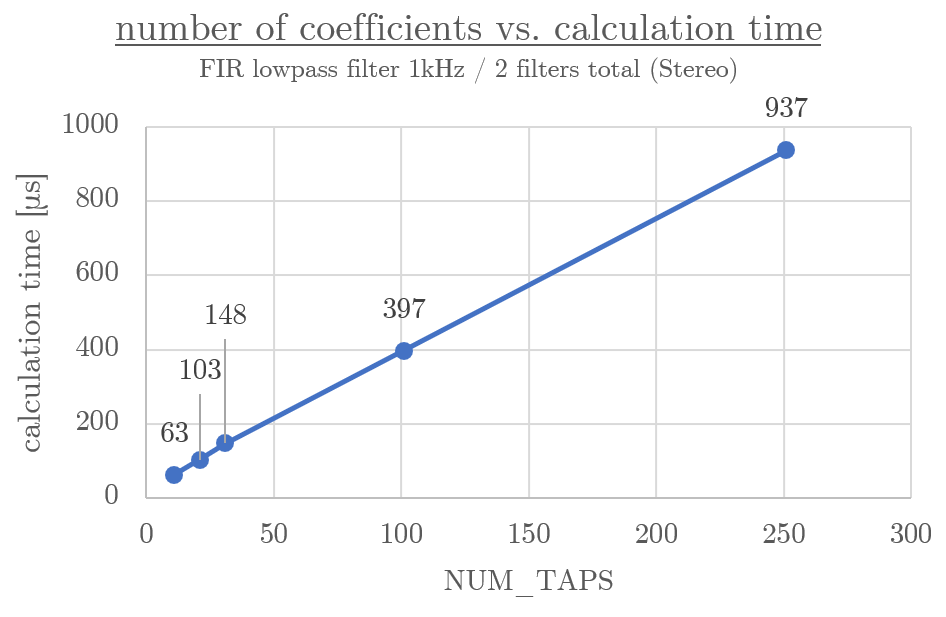
\includegraphics[width=0.8\linewidth]{FIR_NvsT}
	\caption{Die Daten aus Tabelle \ref{tab:FIR_performance} als Grafik dargestellt}
	\label{pic:FIR_NvsT}
\end{figure}

In der Tabelle \ref{tab:FIR_performance} und der Abbildung \ref{pic:FIR_NvsT} ist der Einfluss der Koeffizientenanzahl auf die Performance dargestellt.
Der Zusammenhang der Berechnungszeit und der Länge des Filters ist linear.
Bei der aktuellen Konfiguration mit der Buffergrösse und Samplingrate, können zwei FIR Filter also eine maximale Anzahl Filterkoeffizienten in der Nähe von $1'000$ haben, da sonst die kritische Verarbeitungsdauer von $t_{p}=1.333\si{ms}$ erreicht würde.

Die Abweichung um den Faktor 3 bis 4 in der Effizienz kann aktuell nicht erklärt werden.

\subsubsection{FFT Performance}

Hier wurde nur die FIR Performance behandelt. Relevant für die Beurteilung der FFT Performance ist das Whitepaper von ARM Limited \cite{ARM-Performance-Whitepaper}.

Gemäss den Zahlen im Whitepaper können mit einer Taktfrequenz von $f_{CPU}=100\si{kHz}$ auf einer Cortex-M4 Plattform folgende Werte erzielt werden.

\begin{table}[H]
	\centering
	\begin{tabular}{|c|c|c|}
		\hline
		\textbf{f32 FFT} & \textbf{delay {[}$\mu s${]}} & \textbf{$t_{delay}${[}$\mu\si{s}${]}} \\ \hline
		128              & 7000                & 70                             \\ \hline
		256              & 15000               & 150                            \\ \hline
		512              & 31000               & 310                            \\ \hline
		1024             & 56000               & 560                            \\ \hline
	\end{tabular}
	\caption{float32 FFT Performance auf Cortex-M4 mit 100MHz getaktet}
	\label{tab:FFT_performance}
\end{table}






	\clearpage
	\subsection{Speisung}
\label{subsec:Speisung}

\subsubsection{3.3V-Spannung}
Um die Speisung des Analog- bzw. des Digital-Teils zu verifizieren wurde die Spannung nach den jeweiligen LDOs mit einem Agilent 34410A Multimeter gemessen. Die USB-Versorgungs-Spannung schwankt je nach Quelle zwischen 4.9 und 5.2V, jedoch sollte sie nach den LDOs konstant 3.3V betragen. Gemessen wurden folgende Spannungen:

\begin{equation}
V_{dd_{analog}}=3.2924\si{V}
\end{equation}

\begin{equation}
V_{dd_{digital}}=3.2957\si{V}
\end{equation}

Weiter wurden die Spitzen der Spannungsversorgung mit einem Tektronix TDS 2014C Oszilloskop gemessen. Als Vergleich einmal vom Stromnetz und einmal von einer handelsüblichen Powerbank gespiesen.

\begin{figure} [H]
\begin{minipage}[c]{0.45\textwidth}
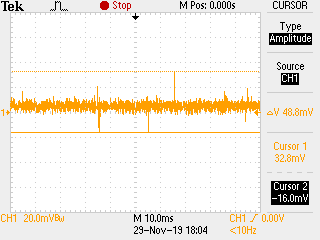
\includegraphics[width=\textwidth]{graphics/Speisung_Netz_Analog.png}
\end{minipage}
\begin{minipage}[c]{0.45\textwidth}
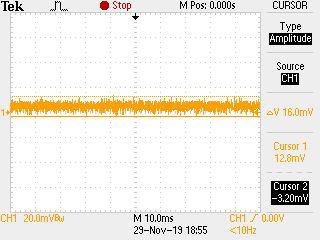
\includegraphics[width=\textwidth]{graphics/Speisung_PB_Analog.png}
\end{minipage}
\caption{Vergleich der analogen Speisung am Netz (links) und mit einer Powerbank (rechts)}
\label{fig:analogspeisung}
\end{figure} 

\begin{figure} [H]
\begin{minipage}[c]{0.45\textwidth}
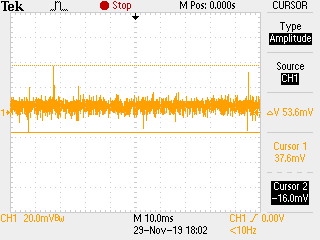
\includegraphics[width=\textwidth]{graphics/Speisung_Netz_Digital.png}
\end{minipage}
\begin{minipage}[c]{0.45\textwidth}
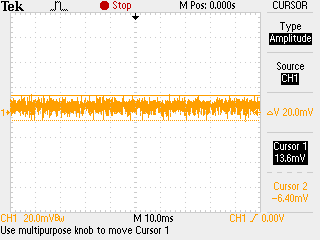
\includegraphics[width=\textwidth]{graphics/Speisung_PB_Digital.png}
\end{minipage}
\caption{Vergleich der digitalen Speisung am Netz (links) und mit einer Powerbank (rechts)}
\label{fig:digitalspeisung}
\end{figure} 

Wie in Abbildungen \ref{fig:analogspeisung} und \ref{fig:digitalspeisung} ersichtlich macht die unterschiedliche Speisung vom Netz sowie der Powerbank einen Unterschied in den Spannungsspitzen. Die Spitzen erreichen 50mV Peak-Peak, was jedoch von den Stützkondensatoren am Microcontroller und am Codec geglättet wird. Das Grundrauschen der Spannung von 20mV ist vertretbar. Die Speisung funktioniert wie erwartet.

\subsubsection{Stromverbrauch}

Die Stromaufnahme der gesamten Schaltung über den Akkumulator wurde mit Hilfe einer Source Measuring Unit (SMU) ermittelt.
Für die Messung lief das DSP Board mit der Demo Software. Beide OLED Displays zeigten Text, die FPU ist eingeschaltet und berechnet ein FIR Filter. Es waren keine Audioquellen oder -senken verbunden.

\begin{table}[H]
	\begin{tabular}{|l|l|l|c|c|}
		\hline
		Messgerät      & Kanal & Prüffmittelnummer & Spannungsbereich & Strombegrenzung \\ \hline
		Agilent N6705B & CH1   & MSZ-M-0064        & 3.7V - 4.2V      & 0.2A            \\ \hline
	\end{tabular}
	\caption{Parameter der SMU}
	\label{tab:SMU_Params}
\end{table}

Der über den gesamten Spannungsbereich von $3.7\si{V}$ bis  $4.2\si{V}$ gemessene Stromverbrauch beläuft sich auf:

\begin{equation}
I_{bat}=64\si{mA}
\end{equation}

Die Stromaufnahme bleibt über den Spannungsbereich konstant, weil die Schaltung die Leistung an der Betriebsspannung von $3.3\si{V}$ konstant bleibt. 
Der Stromfluss durch die LDO's bleibt gleich. Einzig die Verlustleistung an den LDO's steigt mit einer höherer Batteriespannung.




	\subsection{Audio-Schaltung}
\label{subsec:Audio-Schaltung}

Für die Validierung des Analog-Teils wurden verschiedene Teil-Messungen durchgeführt welche nachfolgend erklärt werden.

\subsubsection{Frequenzgang}
\label{subsubsec:Frequenzgang}
Um zu beurteilen ob die Audio-Wandlung und Rückwandlung korrekt funktioniert wird der Frequenzgang der entworfenen Schaltung gemessen. Damit sollte ersichtlich werden welche Frequenz mit welcher Verstärkung von Ein- zu Ausgang übertragen wird. Angestrebt wäre eine möglichst linearer Frequenzgang mit einer Verstärkung von 1 (0dB) auf allen Frequenzen.

\textbf{Anmerkung:} Da am Line-Eingang ein Spannungsteiler die Amplitude des Signals halbiert wurde dies software-mässig korrigiert. Das heisst 0dB in der Software bewirkt eigentlich +6dB am Codec, aber wiederum 0dB auf die ganze Schaltung gesehen wegen des Spannungsteilers.

\begin{figure} [H]
\begin{center}
 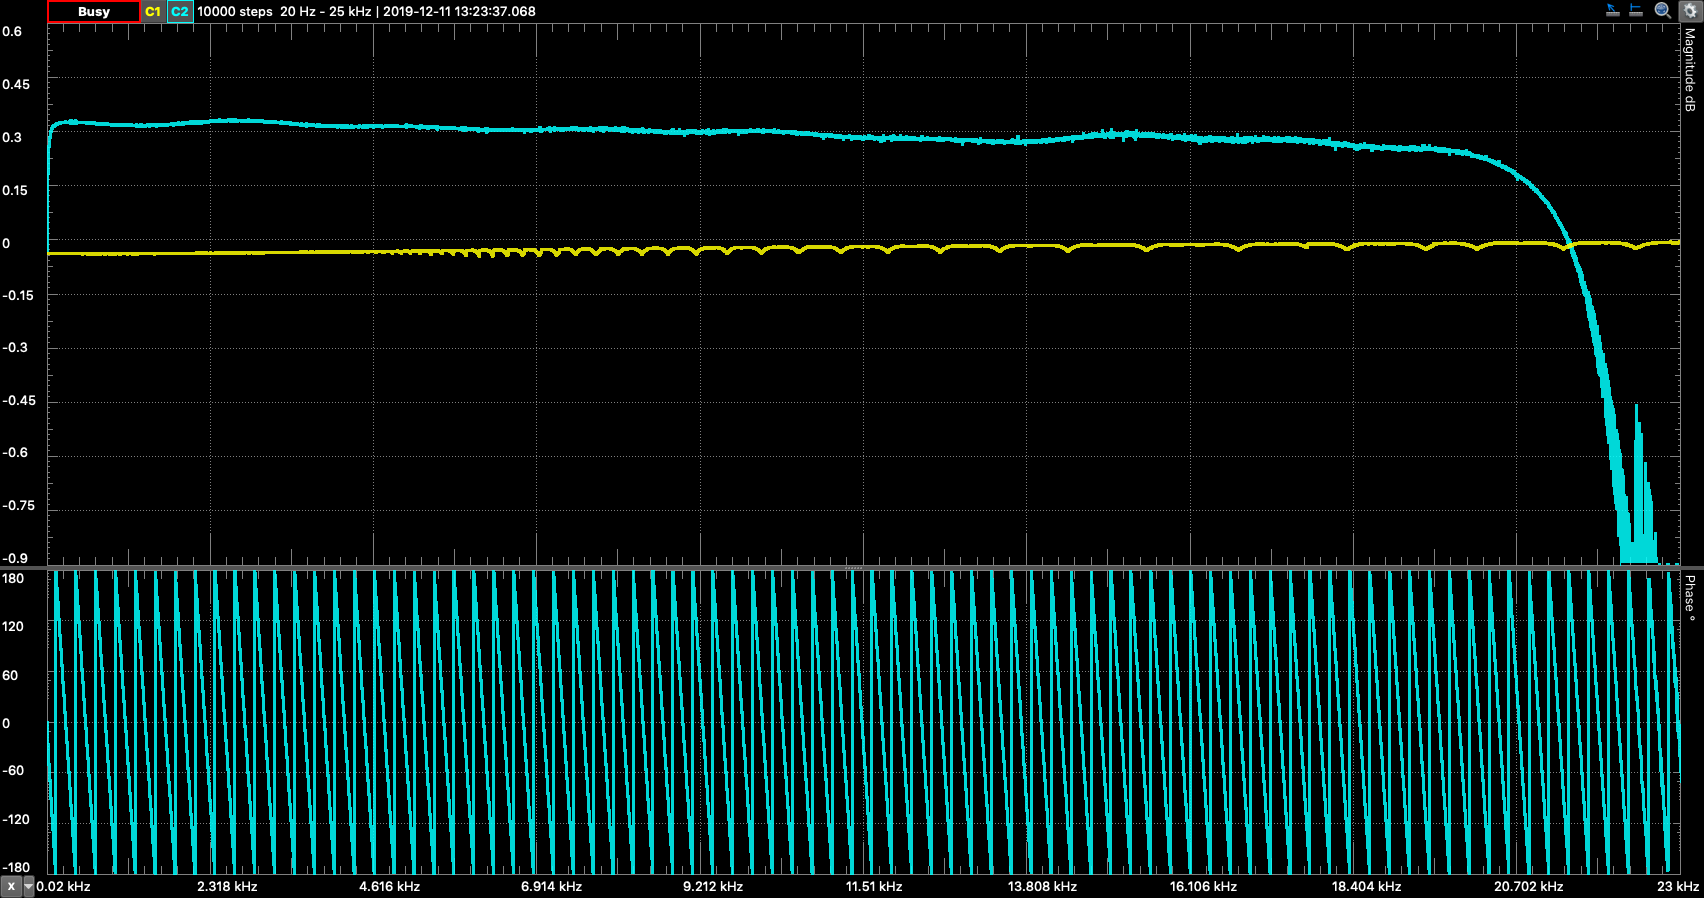
\includegraphics[width=\textwidth]{../graphics/FREQ_LineINOUT.png}
 \caption{Der gemessene Frequenzgang von Audio-Eingang zu Audio-Ausgang (oben) sowie der Phasengang der Schaltung(unten)}
\label{fig:frequenzgang}
\end{center}
\end{figure}
Die Messung wurde mit einem Analog Discovery 2 von Digilent durchgeführt. Der Netzwerk-Analyzer des AD2 generiert hierzu selbst einen Frequenz-Sweep. In \ref{fig:frequenzgang} sieht man das Referenz-Signal (gelb) im Vergleich zur Antwort durch die Schaltung (blau). Wie zu erwarten fängt das Anti-Aliasing-Filter bei der halben Abtastfrequenz (22.05kHz) an zu sperren. Der Phasengang ist wie erwartet linear mit entsprechenden Wrap-around von -180° zu 180°.
Offensichtlich verstärkt die Schaltung um ca. 0.3dB was ein Faktor 1.035 ist. Dies könnte von Wandlungs-Ungenaugkeiten des Codecs herrühren.

\subsubsection{Total Harmonic Distortion}
\label{subsubsec:Total Harmonic Distortion}
Die Total Harmonic Distortion oder auch THD genannt ist ein Leistungs-Verhältnis der harmonischen Oberschwingungen zum ursprünglich  eingespeisten Signal. In diesem Fall ist das eine Sinusschwingung mit einer Frequenz von 1kHz und $2\si{V_{PP}}$ Amplitude (generiert mit einem Agilent 33220A Waveform Generator). Das Signal wird am Eingang eingespiesen, wird einmal AD gewandelt, im Microcontroller 1zu1 kopiert und wieder zurückgewandelt. Am Ausgang wird nun die Amplitudde des Signals im Verhältnis zu dessen harmonischen Vielfachen gemessen.

\begin{equation}
THD_{dB}=20\cdot \log{\frac{THD_{percent}}{100}}
\end{equation} 

\begin{figure} [H]
\begin{center}
 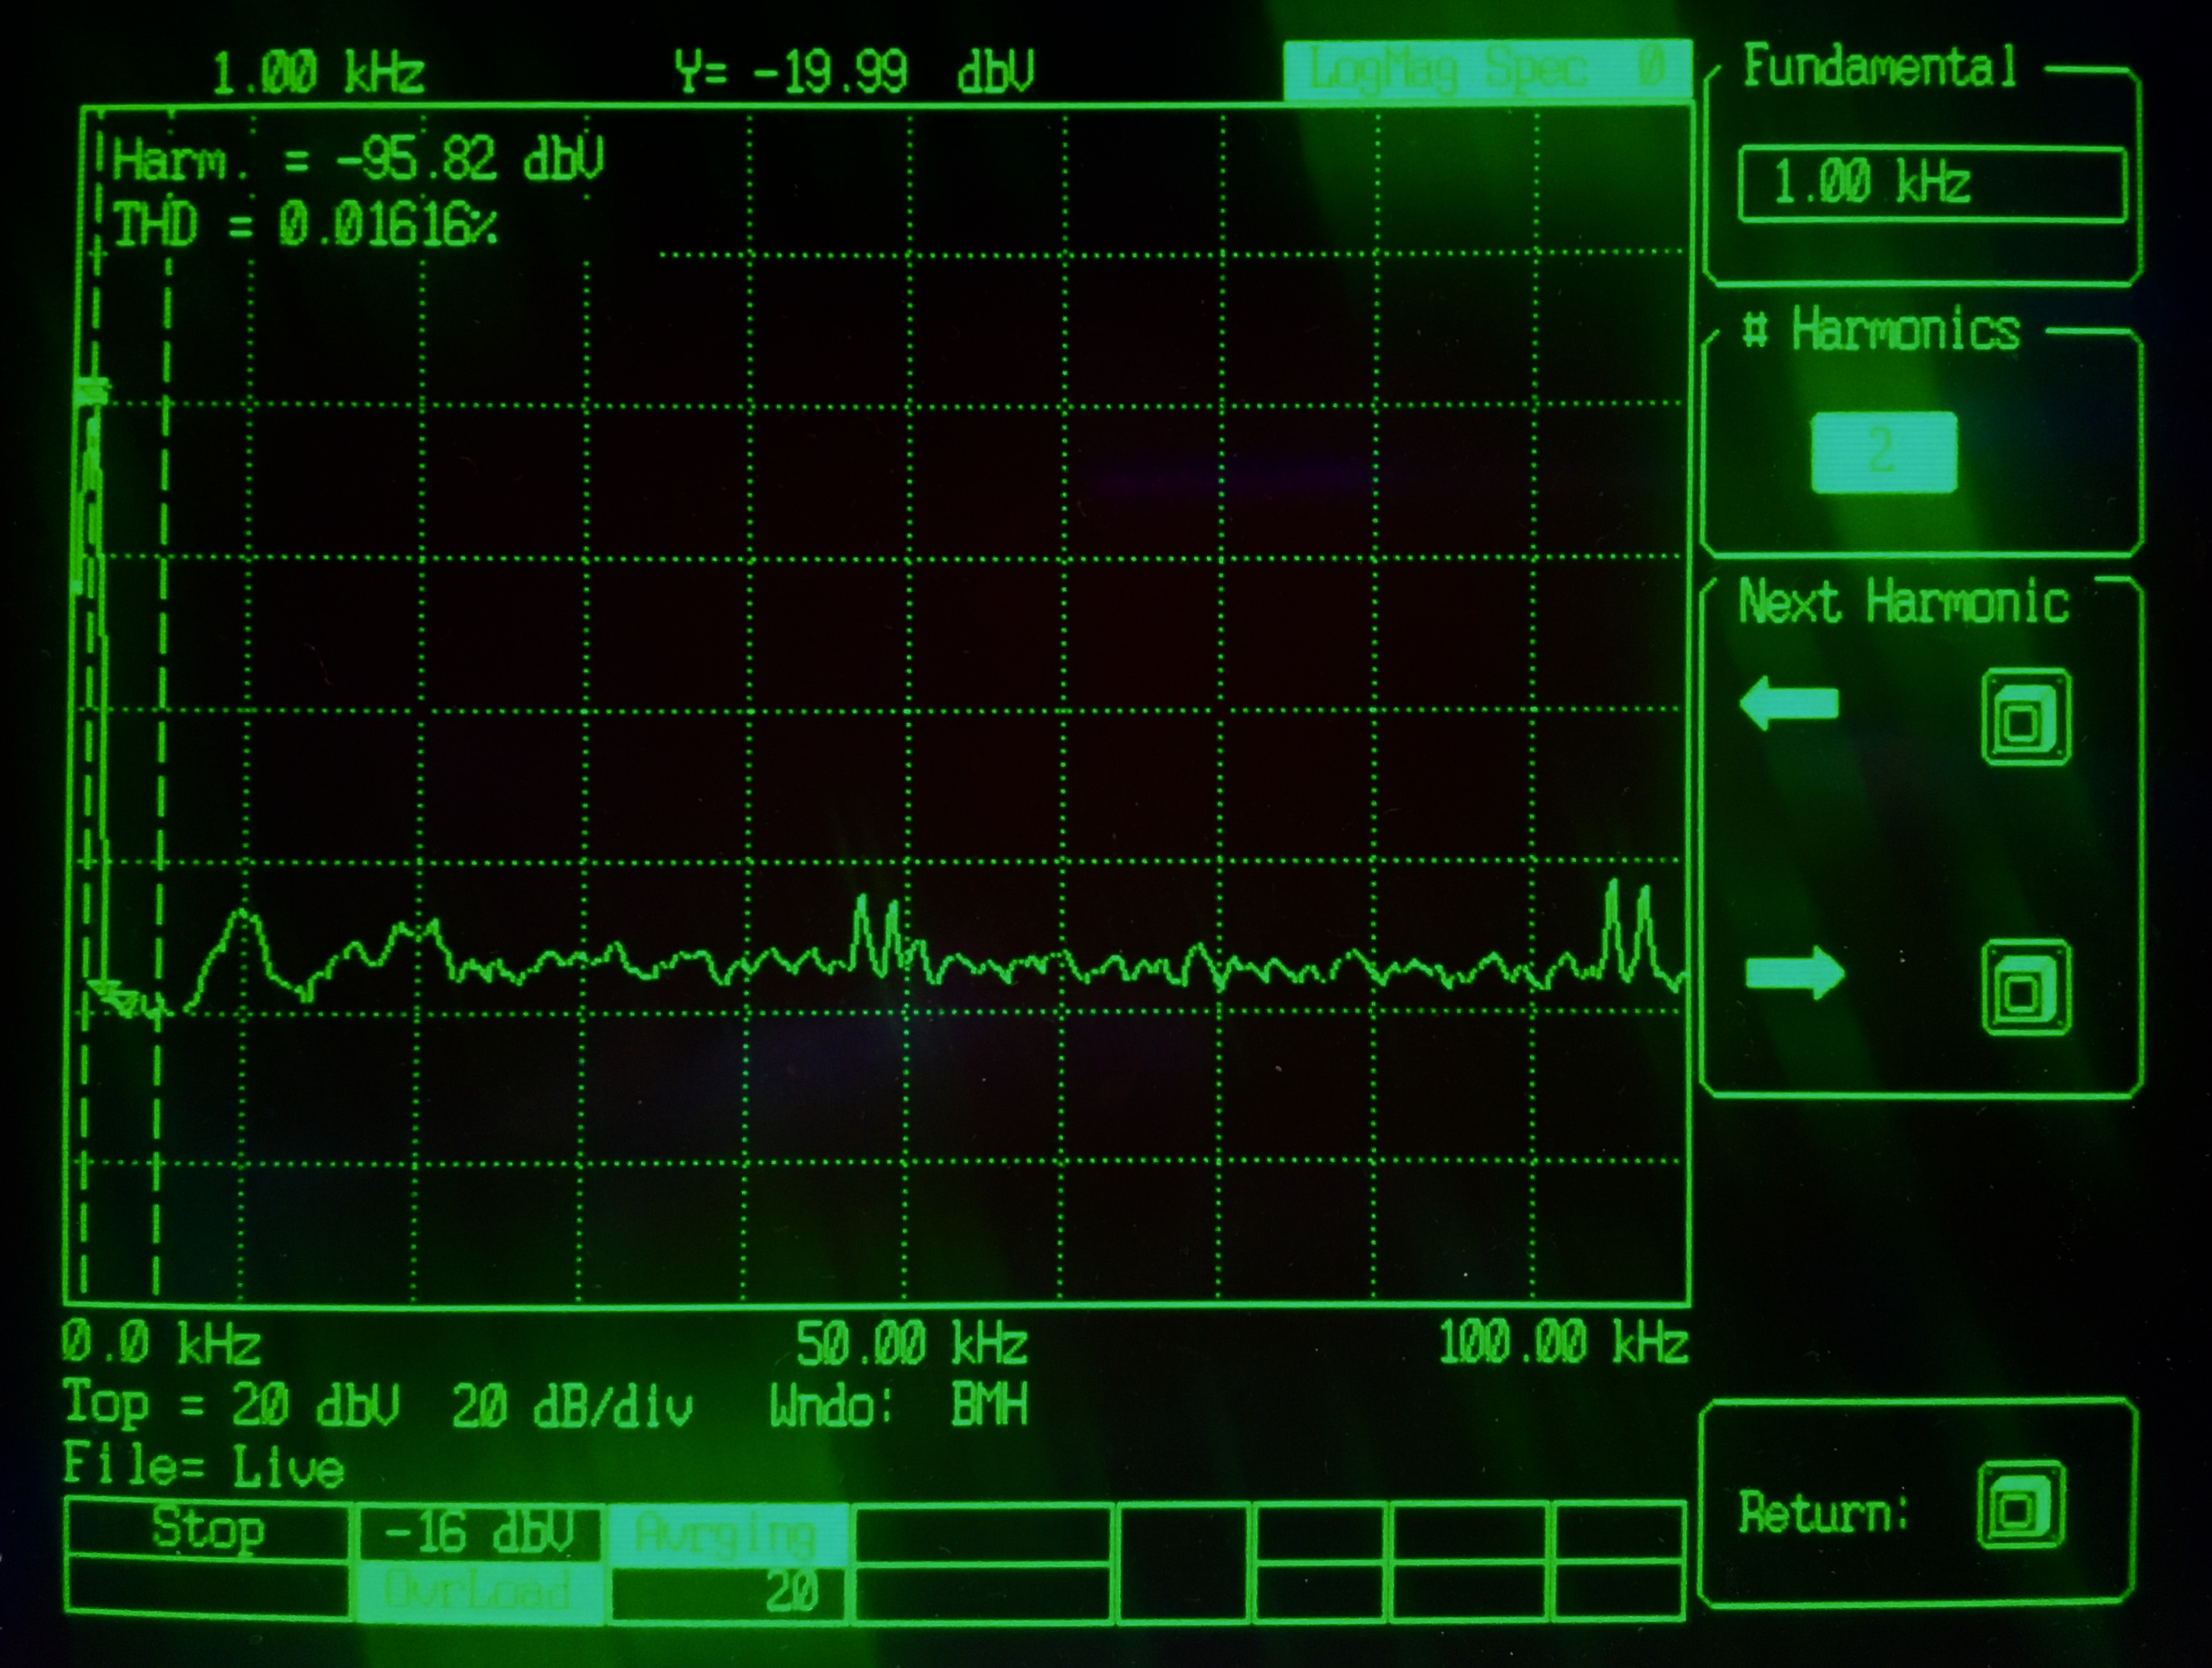
\includegraphics[scale=0.1]{../graphics/THD.jpg}
 \caption{Die gemessene Total Harmonic Distortion mit dem Stanford SR770 FFT Network Analyzer}
\label{fig:thd}
\end{center}
\end{figure}

\begin{equation}
THD_2=75.7744\si{dB}
\end{equation} 

\begin{equation}
THD_5=73.56\si{dB}
\end{equation} 

Die Messung mit dem Stanford SR770 FFT Network Analyzer \ref{fig:thd} ergab eine THD von 0.016\% unter Berücksichtigung von 2 Harmonischen.
Um jedoch die Messung zu verifizieren wird eine zweite Messung mit dem AD2 \ref{fig:thdAD2}  durchgeführt. Diese ergab eine THD von 75.7744dB, was ebenfalls 0.016\% entspricht. Betrachtet man fünf harmonische Vielfache erhöht sich die THD nur leicht auf 0.021\%. Das heisst die ersten fünf harmonische Vielfachen des 1kHz Sinus tragen nicht einmal ein tausendstel zum übertragenen Signal bei.

\begin{figure} [H]
\begin{center}
 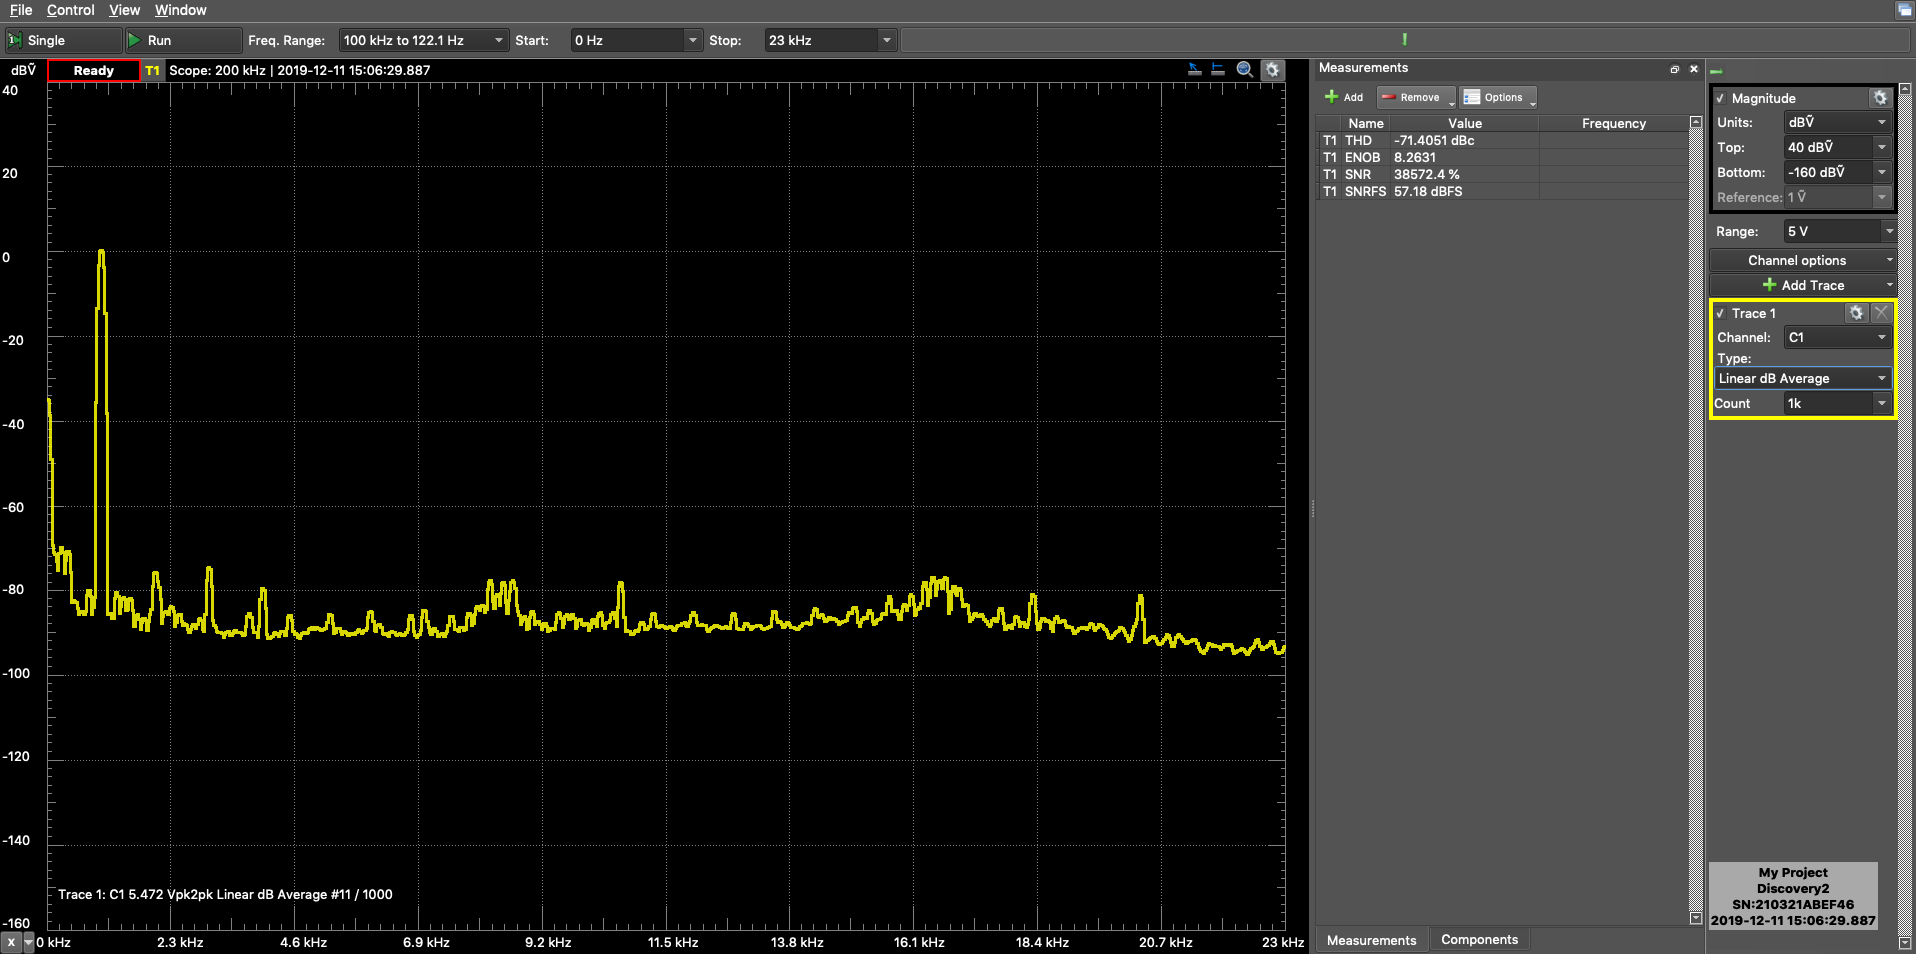
\includegraphics[width=\textwidth]{../graphics/THD_LineINOUT.png}
 \caption{Die gemessene Total Harmonic Distortion mit dem Analog Discovery 2 von Digilent}
\label{fig:thdAD2}
\end{center}
\end{figure}

\subsubsection{ENOB/SINAD}
\label{subsubsec:ENOB/SINAD}

Die \glqq Effective number of bits\grqq, oder kurz ENOB genannt, gibt an wieviel Bits an Auflösung eines AD-Wandlers effektiv nutzbar sind. Durch Rauschen verschiedener Art, sei es von der Quantisierung oder von Widerständen, hat der Wandler-Kanal einen gewissen Grundpegel der nicht für Information genutzt werden kann. Entsprechend sinkt der Amplitudenbereich in dem Information eines Signals übertragen werden kann. Sozusagen die effektive Anzahl nutzbarer Bits (wie es der Name schon sagt).

Der SINAD, oder auch \glqq Signal-to-interference ratio including noise and distortion\grqq , ist das Leistungs-Verhältnis  von Rauschen und den harmonischen Verzerrungen zum Signal (wie der SNR, aber mit Distortion). Er steht auch in direktem Verhältnis zum ENOB:

\begin{equation}
ENOB=\frac{SINAD-1.76dB}{6.02dB}=11.23\si{bit}
\end{equation} 

Beide Werte wurden ebenfalls mit dem AD2 gemessen. Beim SINAD ergab das einen Wert von 69.367dB und für den ENOB 11.23. Gerade für den ENOB ist dieser wert enttäuschend für einen 16 Bit ADC. Ein Grund dafür könnte die Messkette sein, da von Eingang zu Ausgang gemessen wurde. Sprich das Signal wurde zweimal gewandelt und erfährt dementsprechend auch mehr Rauschen. 
\clearpage
\section{Status und Verbesserungen}
\label{sec:Status}

\subsection{Aktueller Status des DSP Boards}


\subsection{Nächste Schritte}

Nachfolgend ist aufgelistet, welche Fehler und Probleme mit der jetzigen Hardware bestehen.

\paragraph{Pull-Up Widerstände in digitalen Signalen}

Einige Signale haben im Schema keinen Pull-Up oder Pull-Down Widerstand verbaut.

\todo{Welche Signalleitungen?}

\paragraph{Analoge Speisung muss immer enabled sein}

Ursprünglich war angedacht, dass der analoge Schaltungsteil über den Enable des LDO ausgeschaltet werden kann. Dies funktioniert nicht, da der STM32 ebenfalls eine stabile analoge Speisung benötigt. Fällt die analoge Speisung weg, fällt der STM32 in einen Reset-Loop.
Die neue Hardware benötigt ein neues Konzept für den Energiesparmodus.

\paragraph{Kompatibilität des AVX Steckers mit einem Gehäuse}

Die Beiden AVX Stecker für die Kaskadierung sind genau an der Kante des PCBs montiert. Dadurch müssen zwei Boards Kante an Kante nebeneinander platziert werden.
Ein Gehäuse, dass die PCB Kante einschliesst, kann deshalb nicht verbaut werden.
Das Konzept mit den Steckverbindern muss nochmals überarbeitet werden.
Der Vorschlag lautet: AVX Stecker beibehalten und die PCB-Kante beim Stecker um einige Millimeter nach aussen versetzen (PCB-Form nicht rechteckig).

\paragraph{Kühlfläche für BQ2409x}

Der BQ2409x hat auf der Unterseite ein Kühlpad. Die Kühlung des Chips ist in diesem Projekt nicht beachtet worden. Dadurch kann die Ladefunktion des Chips infolge thermischer Überlastung nicht genutzt werden. Die nächste Hardwareiteration benötigt eine Kühlfläche und den korrekten Footprint mit Kühlpad.

\paragraph{Blockkondensator für ADC Pin (Batteriespannung)}

Der Spannungsteiler für die Batteriespannungsmessung benötigt einen Blockkondensator um AC-Noise zu filtern. Der Kondensator soll idealerweise nahe am STM32 platziert sein.

\paragraph{JST-Battery Connector}

Der JST-Stecker ist ebenfalls zur Überarbeitung ausgeschrieben. Hier braucht es den korrekten Stecker, der auch zum entsprechenden Akku passt. 
Der aktuell auf der Stückliste ausgeschriebene Steckertyp ist zu gross für den testweise bestellten Akkumulator.

\todo{Mic-Bias-Schaltung ist falsch (nur für Electret, aber auf 2 Kanäle) / DTCT auch ändern}

\paragraph{Überspannungsschutz für Audio-Eingang}

Die Audio-Eingänge des TLV320 halten maximal $1\si{V_{RMS}}$ aus. Die Eingänge könnten sehr einfach mit deiner Schaltung aus zwei antiparallel geschalteten Leuchtdioden vor zu grossen Spannungen geschützt werden. LEDs eignen sich aufgrund des geringen Leckstromes und einer Durchlassspannung im Bereich 1.5V besonders gut für diese Anwendung.
Die Mehrkosten und Nutzen der Schutzschaltung sind abzuwägen.

\todo{TLV320 Lautstärke bei +12dB auf Mute}


% müssen die folgenden Punkte dokumentiert werden?
% \todo{Audio-Switch auf Board 4 auswechseln (schaltet nur eine Seite)}
\clearpage

%\section{Schluss}
\label{sec:Schluss}
\todo[inline]{Gegenlesen - Fertig - MR -  In diesem Kapitel steht die Zusammenfassung des Resultats und inwiefern die Projektziele damit erfüllt sind (mit Verweis auf die Validierung). Ebenfalls wird das Weiterentwicklungspotential aufgezeigt. - A: MR}

Anhand der Mechanik des 3D Druckers Ender 3 Pro und der eigens gefertigten Steuerung konnte ein robuster, leistungsfähiger und einfach zu bedienender Drucker entwickelt und in Betrieb genommen werden (siehe Kapitel \ref{sec:Validierung}). Neben allen definierten Sollzielen konnten auch alle Wunschziele umgesetzt werden.

Der Benutzer kann seine G-Code Files nun nicht nur per SD-Karte, sondern auch per Fernzugriff über das Webinterface auf den Drucker laden und den Druck auch gleich starten. Über den Druckfortschritt wird er auf dem Display des Druckers oder auch auf dem Webinterface informiert. Die beiden horizontalen Achsen des Druckers (X- und Y-Achse) werden ohne Endschalter referenziert. Dadurch ist die Anzahl der  Sensoren reduziert.
Der verwendete 32-Bit Prozessor verfügt über genug Rechenleistung, sodass zukünftig auch Erweiterungen vorgenommen werden können, die rechenaufwändig sind. Des Weiteren können Updates der Firmware über das Webinterface getätigt werden. Ungenutze Pins des Prozessors sind auf Headers geführt, wodurch die Implementierung eines weiteren Motors einfach umzusetzen ist und kaum Hardwareanpassungen benötigt werden.

Die verwendete Firmeware, Marlin, kommt im Hobbybereich häufig zum Einsatz, was der Realisierung dieses Projekts zu Hilfe kam. Für diverse Herausforderungen konnten online Lösungen gefunden  oder gar Unterstützung durch die Entwickler in Anspruch genommen werden. Für den professionellen Gebrauch sei an dieser Stelle aber von Marlin abzuraten, weil es sich um eine Open-Source-Software handelt, deren Übersichtlichkeit zu Wünschen übrig lässt.

Alles in Allem darf gesagt werden, dass das Projekt 4 erfolgreich durchgeführt werden konnte und der Drucker nach Abschluss des Projekts mit Stolz der FHNW übergeben wird.
\clearpage
%\section{Ehrlichkeitserklärung}
\label{sec:Ehrlichkeitserklärung}

Hiermit erklären wir, die vorliegende Arbeit selbständig, ohne Hilfe Dritter und nur unter Benutzung der
angegebenen Quellen verfasst zu haben.

\vspace{2cm}
Windisch, \today :  
\vspace{1cm} 
\begin{table}[h!]
\def\arraystretch{2}
\begin{tabular}{llL{6cm}}
Tobias Blum			 &  & \\ \cline{3-3} 
					 &  &	\\
Simon Burkhardt       &  &  \\ \cline{3-3} 
					 &  &	\\
Olivier Lutz         &  &  \\ \cline{3-3}
					 &  &	\\
Marco Meier          &  &  \\ \cline{3-3}
					 &  &	\\
Dominik Müller       &  &  \\ \cline{3-3}
					 &  &	\\
Michael Ramseier     &  &  \\ \cline{3-3}
					 &  &	\\
Marco Thommen		 &  &  \\ \cline{3-3}               
\end{tabular}
\end{table}




%%---BIBLIOGRAPHY------------------------------------------------------------------------
\clearpage

{\sloppypar
\printbibliography
\label{sec:lit}
}


%%---APPENDIX----------------------------------------------------------------------------
\begin{appendix} %Anhang
\section{Anhang}
\label{sec:Anhang}

\subsection{Schema}
\label{app:Schema}

\begin{figure}[h!]
	\centering
	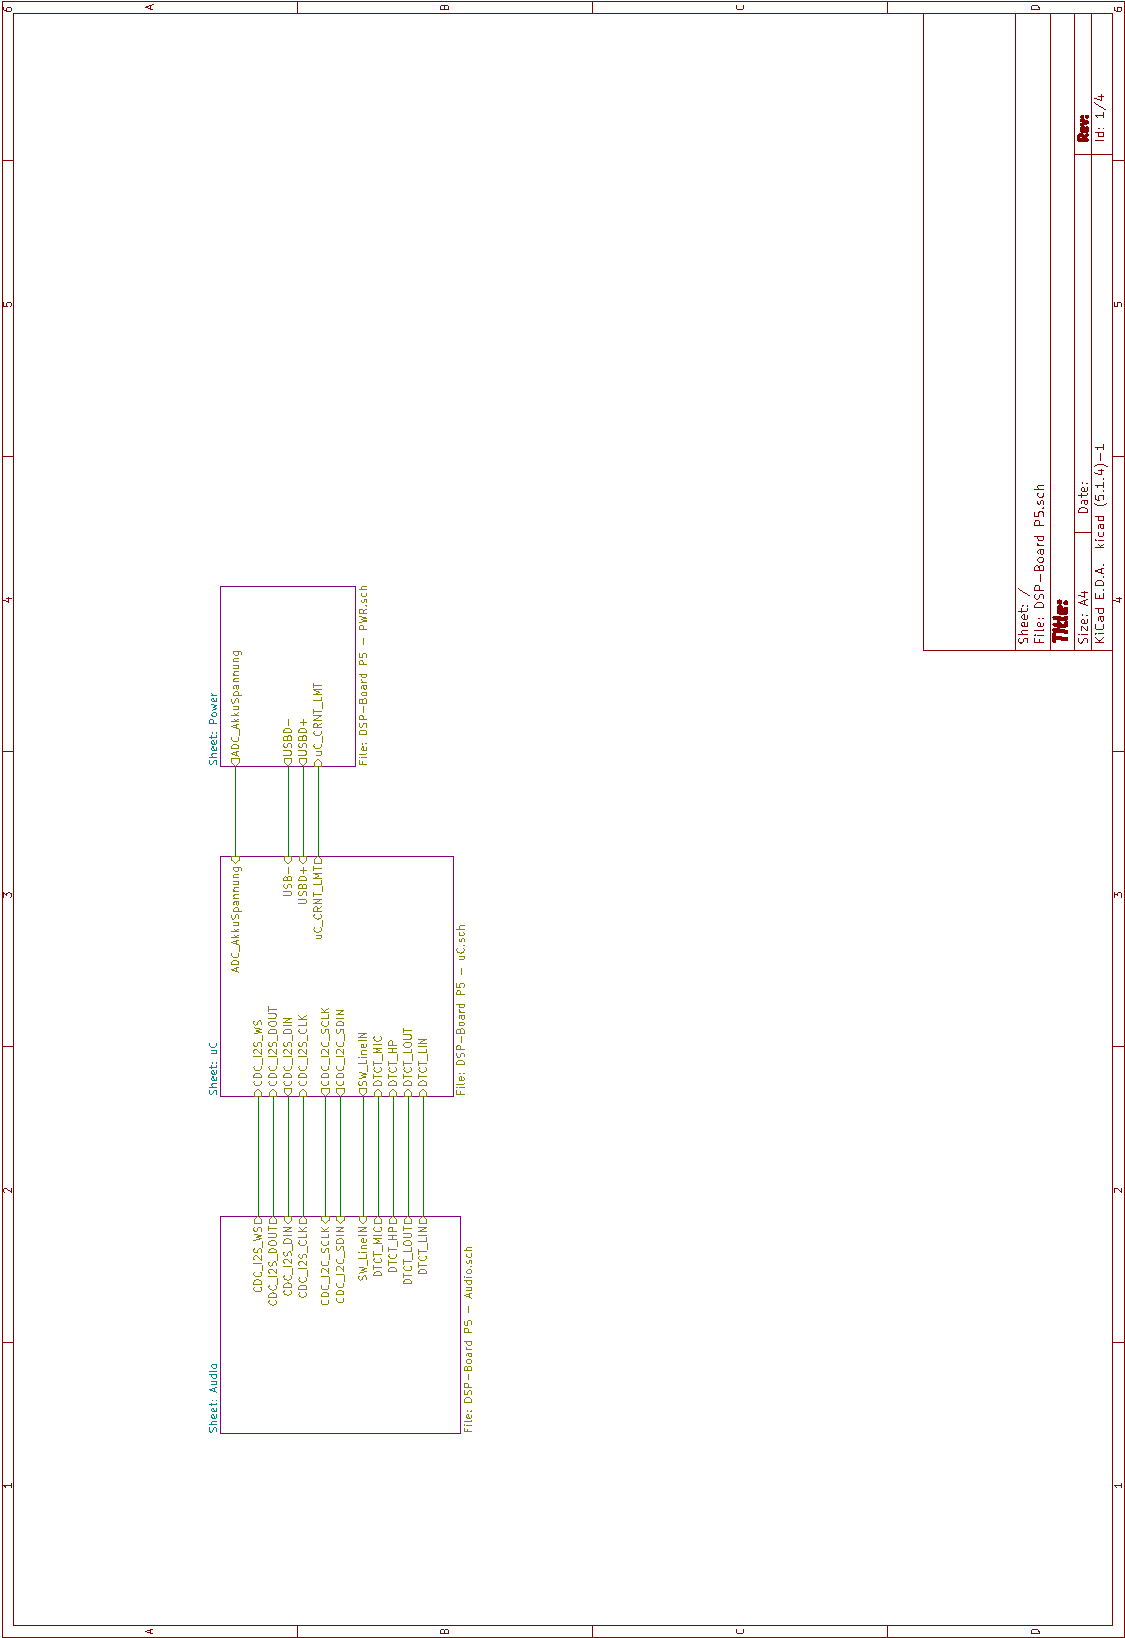
\includegraphics[width=0.95\linewidth]{appendix/DSP-Board-Schema-V1-1(1).pdf}
\end{figure}

\begin{figure}[h]
	\centering
	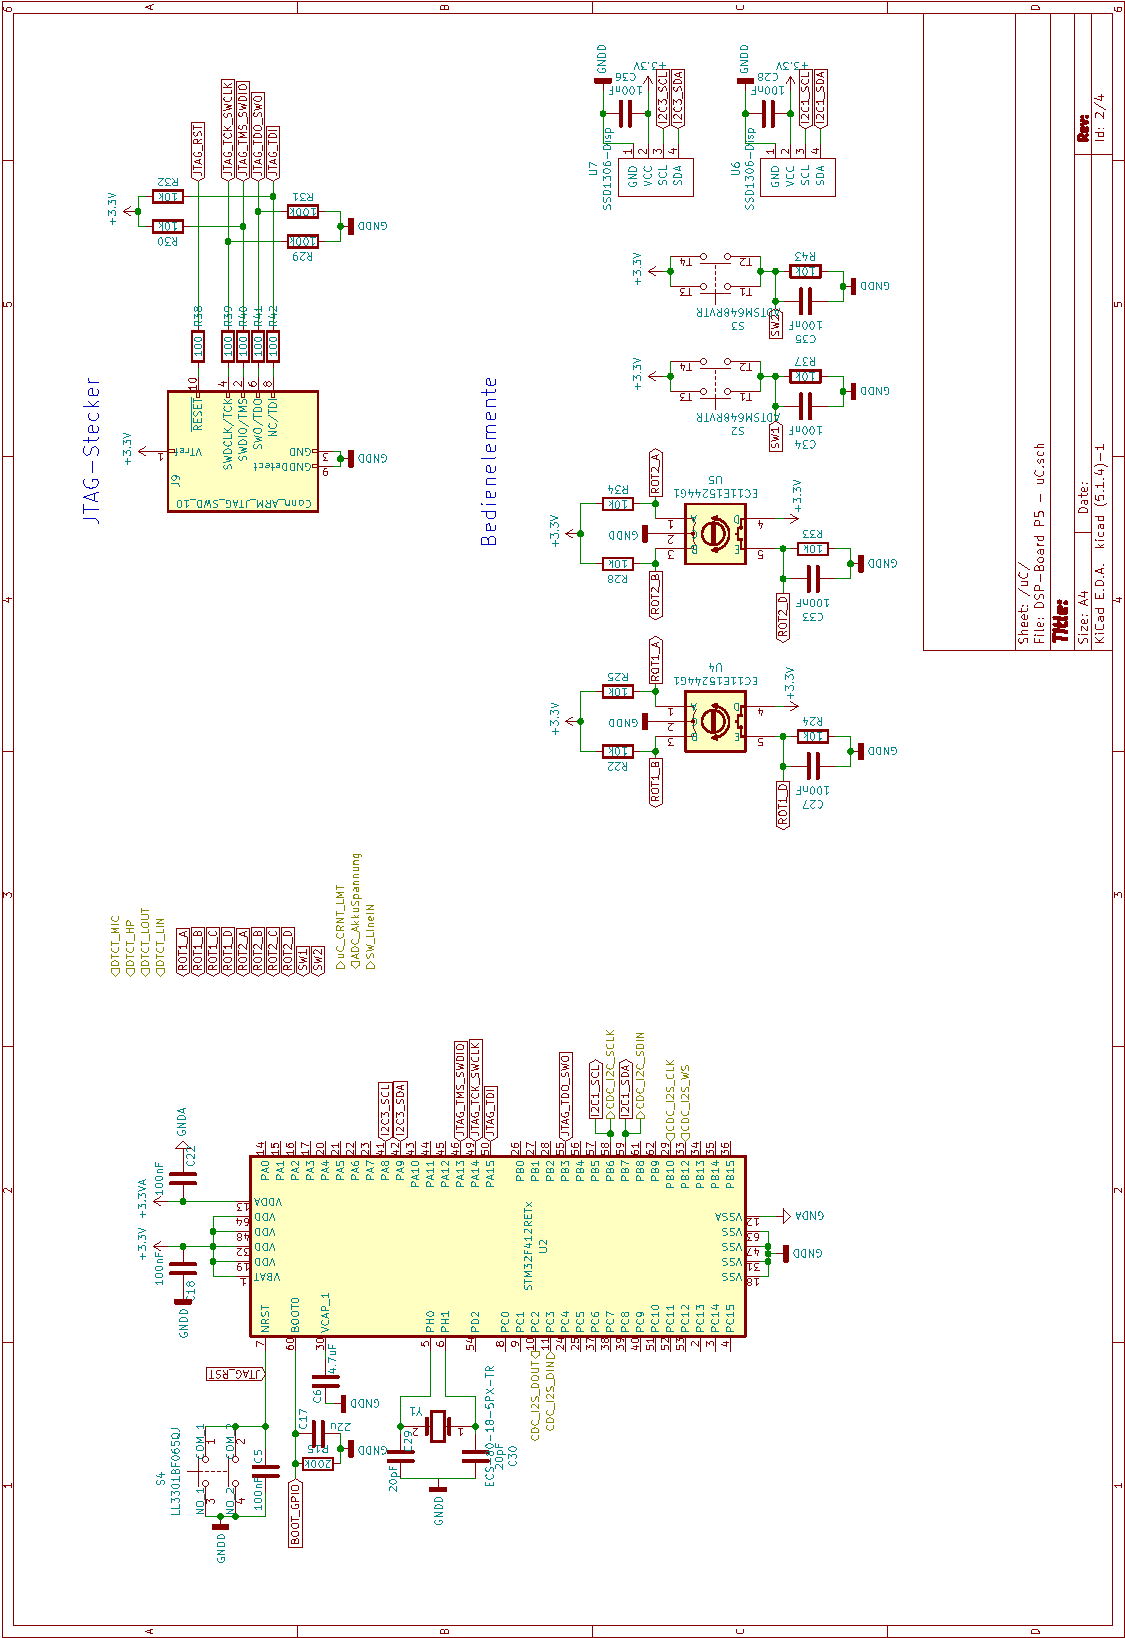
\includegraphics[width=0.95\linewidth]{appendix/DSP-Board-Schema-V1-1(2).pdf}
\end{figure}

\begin{figure}[h]
	\centering
	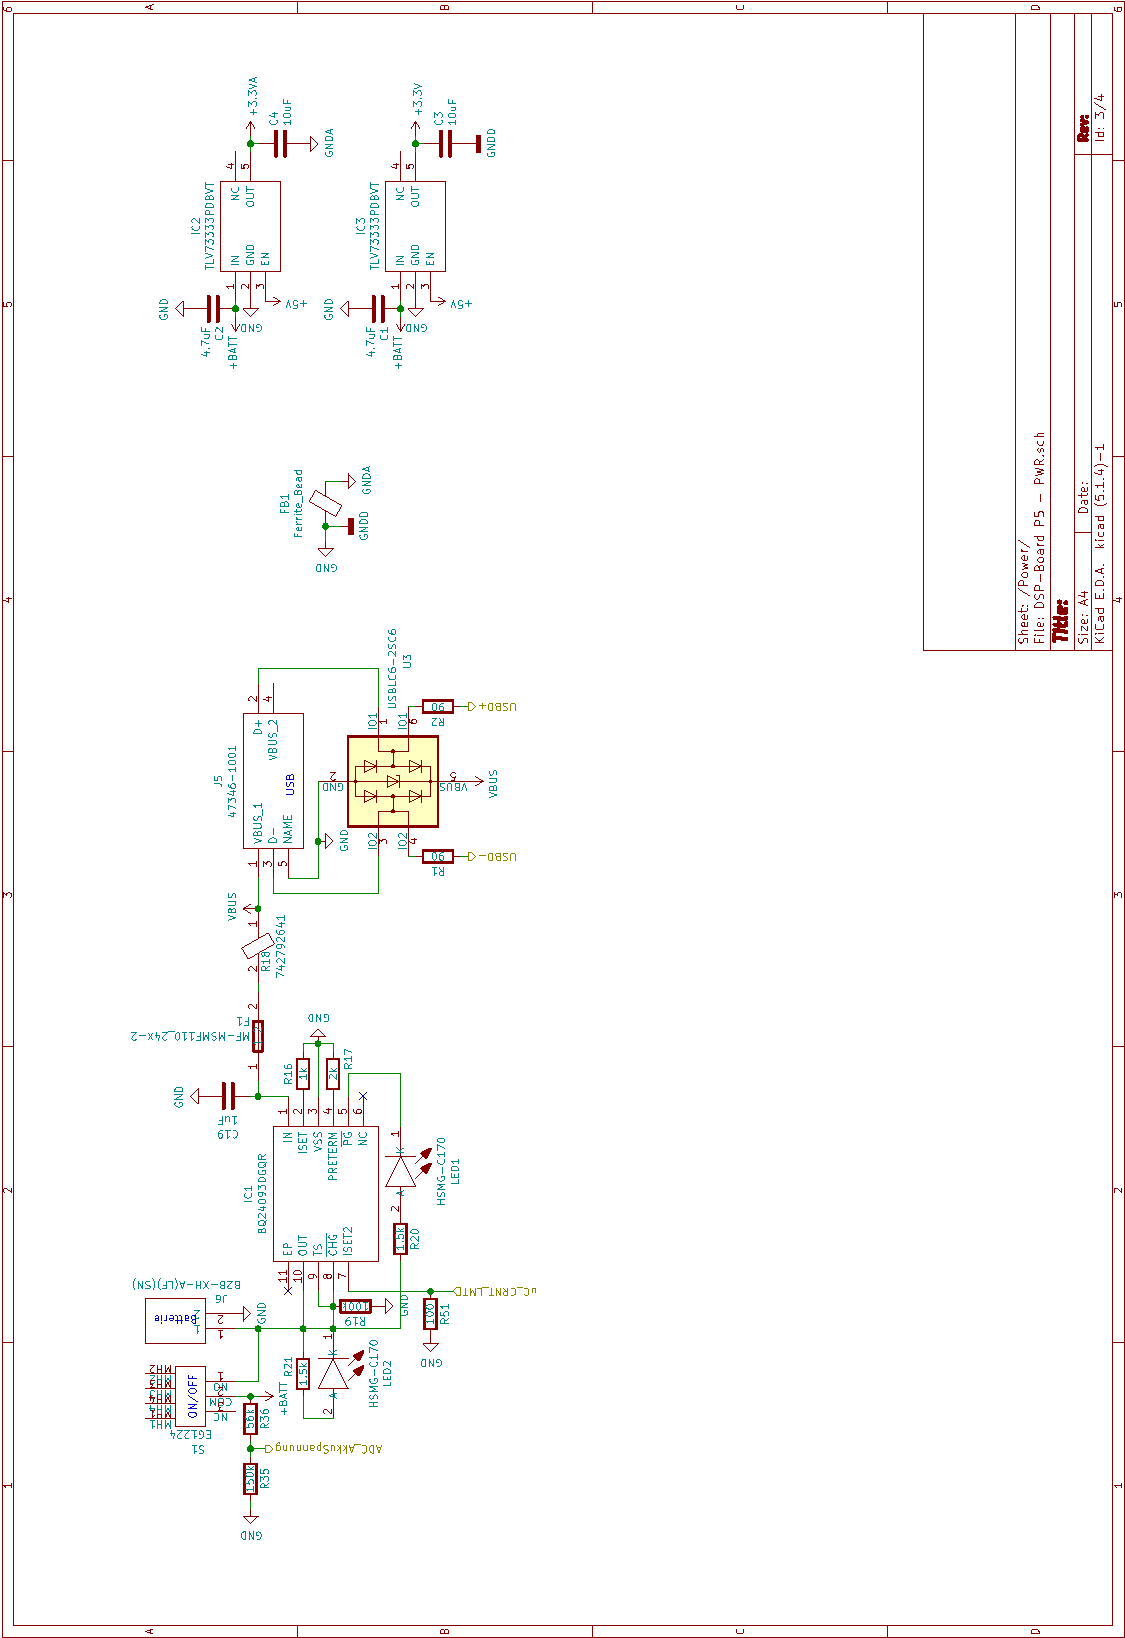
\includegraphics[width=0.95\linewidth]{appendix/DSP-Board-Schema-V1-1(3).pdf}
\end{figure}

\begin{figure}[h]
	\centering
	\includegraphics[width=0.95\linewidth]{appendix/DSP-Board-Schema-V1-1(4).pdf}
\end{figure}

\clearpage

\subsection{PCB Layout}
\label{app:PCB}

\begin{figure}[h!]
	\centering
	\includegraphics[width=0.95\linewidth]{appendix/DSP-Board-PCB-V1-1(1).pdf}
\end{figure}

\begin{figure}[h]
	\centering
	\includegraphics[width=0.95\linewidth]{appendix/DSP-Board-PCB-V1-1(2).pdf}
\end{figure}

\begin{figure}[h]
	\centering
	\includegraphics[width=0.95\linewidth]{appendix/DSP-Board-PCB-V1-1(3).pdf}
\end{figure}

\begin{figure}[h]
	\centering
	\includegraphics[width=0.95\linewidth]{appendix/DSP-Board-PCB-V1-1(4).pdf}
\end{figure}
\clearpage

\subsection{Pflichtenheft}
\label{app:Pflichtenheft}

\begin{figure}[h!]
	\centering
	\includegraphics[width=0.95\linewidth]{appendix/pflichtenheft(1).pdf}
\end{figure}

\begin{figure}[h]
	\centering
	\includegraphics[width=0.95\linewidth]{appendix/pflichtenheft(2).pdf}
\end{figure}

\begin{figure}[h]
	\centering
	\includegraphics[width=0.95\linewidth]{appendix/pflichtenheft(3).pdf}
\end{figure}

\begin{figure}[h]
	\centering
	\includegraphics[width=0.95\linewidth]{appendix/pflichtenheft(4).pdf}
\end{figure}

\begin{figure}[h]
	\centering
	\includegraphics[width=0.95\linewidth]{appendix/pflichtenheft(5).pdf}
\end{figure}

\begin{figure}[h]
	\centering
	\includegraphics[width=0.95\linewidth]{appendix/pflichtenheft(6).pdf}
\end{figure}


\end{appendix}










%%---NOTES for DEBUG---------------------------------------------------------------------
%
\newpage
\listoftodos[\section{Todo-Notes}]
\clearpage


\end{document}